\chapter{Redes neuronales artificiales evolutivas multi-objetivo}\label{MOEANNs}
% \begin{quotation}
% \begin{small}
% 		\textit{El pesimista es un optimista con experiencia.}\\
% 		\textit{El pesimista es una persona previsora y bien informada.}
% \end{small}
% \begin{flushright}
% François Truffant.\\
% Anónimo.
% \end{flushright}
% \end{quotation}
\section{Algoritmos evolutivos multi-objetivo}\label{multiobjetivo}
\noindent  En ocasiones necesitamos resolver problemas con varios
objetivos a optimizar, generalmente contrapuestos, y a veces, sin  ningún  conocimiento
“a priori” de  cómo  interactúan entre sí. Son problemas de este tipo: maximizar
beneficios y minimizar costes de un producto, maximizar el desarrollo y minimizar el
consumo de gasolina de un vehículo, minimizar el peso y maximizar la fortaleza de un
componente, etc.
A estos problemas se les llama problemas de optimización multi-objetivo
(\textit{Multi-objective Optimization Problems}, MOPs) \cite{Deb2004,Coello2007}.

Mientras que en optimización mono-objetivo se busca un vector de decisión $n$-dimensional
que optimice una función escalar, en optimización multi-objetivo se intenta encontrar un
vector que optimice una función vectorial cuyos elementos representan las distintas
funciones objetivo.

A continuación definiremos qué es un MOP, así como una serie de conceptos esenciales en la
optimización multi-objetivo.
\newpage
\subsection{Optimalidad de Pareto}
\noindent
\begin{description}
\item[Definición 1. Problema de optimización multi-objetivo:] El problema de optimización
multi-objetivo se puede formular, de forma general, como el problema de encontrar el
vector
$\displaystyle \mathbf{x}^* = \left[ x^*_{1},x^*_{2},\cdots,x^*_{n}\right]^T $ que
satisfaga
las $m$ restricciones de desigualdad:
\begin{displaymath}
g_{i}(\mathbf{x})\geq0 \quad i=1,2,\cdots,m
\end{displaymath}
Las $p$ restricciones de igualdad
\begin{displaymath}
h_{i}(\mathbf{x})=0 \quad i=1,2,\cdots,p
\end{displaymath}
y que optimice
\begin{displaymath}
f(\mathbf{x})= \left[
f_{1}(\mathbf{x}),f_{2}(\mathbf{x}),\cdots,f_{k}(\mathbf{x})\right] ^T
\end{displaymath}
La solución de un MOP minimiza o maximiza (según corresponda) los componentes del vector
$f(\mathbf{x})$. Por tanto, el problema tiene $k$ objetivos y las funciones
$\displaystyle f(\cdot): \Omega \rightarrow A$ representan la correspondencia entre el
espacio
de búsqueda $\Omega$  y el espacio de las funciones objetivo $A$. De la definición de MOP
se infiere que la solución del problema puede no ser única, ya que los diversos
objetivos pueden estar en conflicto, de forma que la optimización de uno de ellos lleva,
en general, a un
descenso del valor de otro.
% De hecho, la optimización global de un problema multi-objetivo
% es un problema
% NP-completo.
\item[Definición 2. Optimalidad de Pareto:] Decimos que un punto $\mathbf{x}^* \in \Omega$
es
un óptimo de Pareto si para todo $\mathbf{x}^* \in \Omega \quad e \quad I=\left\lbrace
	1,2,\cdots,k\right\rbrace$ se verifica que $\displaystyle \forall_{i}\in I,\left(
	f_{i}\left(\mathbf{x})\right) = f_{i}\left( \vec x^*\right) \right) $ o $\exists$ $i
\in	I$ tal que $\displaystyle f_{i}(\mathbf{x})>f_{i}(\mathbf{x}^*)$.
\item[Definición 3. Dominancia de Pareto:] En un problema de minimización, un vector
$\displaystyle \mathbf{u} =\left( u_{1},u_{2},\cdots,u_{k}\right) \in A \subseteq \Re^n$
domina a otro $\displaystyle \mathbf{v} =\left( v_{1},v_{2},\cdots,v_{k}\right)$ $\in A
\subseteq \Re^n$ (denotado mediante $\displaystyle \mathbf{u} \succeq \mathbf{v}$), si y
solo si, $u$ es parcialmente menor a $v$, es decir, $\displaystyle \forall_{i} \in \left\lbrace
1,\cdots,k\right\rbrace,
\quad u_{i}\leq v_{i} \wedge \exists \quad i \in \left\lbrace 1,\cdots,k\right\rbrace
\text{ tal que } u_{i}<v_{i}$.
\item[Definición 4. Conjuntos de óptimos de Pareto:] Para un problema multi-objetivo dado
$\displaystyle \mathbf{f} (x)$, el conjunto de óptimos de Pareto $\left( \mathcal{P}^*
\right)$ se define como:
\begin{displaymath}
\mathcal{P}^*:=\left\lbrace x\in \Omega \mid \nexists  x' \in
\Omega \quad \text{tal que } \mathbf{f}\left( x'\right)  \preceq
\mathbf{f}\left(x\right)\right\rbrace
\end{displaymath}
\item[Definición 5. Frente óptimo de Pareto:] Para un problema multi-objetivo dado
$\mathbf{f}(x)$ y un conjunto de óptimos de Pareto $\mathcal{P}^*$, el frente de Pareto
$\left(
\mathcal{P}\mathcal{F}^* \right)$ se define como:
\begin{displaymath}
\left(
\mathcal{P}\mathcal{F}^* \right):=\left\lbrace \mathbf{u}=\mathbf{f}= \left( f_{1}\left(
x\right)
,\cdots,f_{k}\left( x\right)\right)  \arrowvert x \in \mathcal{P}^*\right\rbrace
\end{displaymath}
\item[Definición 6. Mínimo global de un MOP:] Dado un vector de funciones
$\displaystyle f(\cdot): \Omega \subseteq \Re^k \rightarrow \Re^n, \quad \Omega \neq 0,
\text{ y } k\geq2$, se llama al conjunto $\displaystyle \mathcal{P}\mathcal{F}^* :f(x^*)$
mínimo global, si y sólo si, $\displaystyle \forall x \in \Omega : f(x^*) \prec f(x)$,
donde $x^* \in \Omega $ se llama conjunto de soluciones de mínimo global,
$\displaystyle f(\cdot)$ es el vector de funciones objetivos y $\Omega$ el espacio de
búsqueda.

A raíz de estas definiciones se deduce que el mínimo global es la frontera de
Pareto del problema y las soluciones de mínimo global forman el conjunto de óptimos
de Pareto. Un problema de optimización de Pareto donde el espacio de búsqueda es $\Re^k$,
tiene, en general, infinitas soluciones.
\item[Definición 7. Dominancia débil y fuerte:] Un vector es un óptimo de Pareto débil si
no existe otro vector para el cual todos sus componentes en el espacio de las funciones
objetivo sean mejores. De manera formal, se puede definir como sigue:
\begin{itemize}
	\item \textbf{No dominancia débil}: Una solución $\displaystyle \mathbf{x}^* \in
\Omega $
es una solución débilmente no dominada si no existe otra solución $\displaystyle
\mathbf{x}
\in \Omega$ tal que $\displaystyle f_{i}(\vec x) < f_{i}(\mathbf{x}^*), \quad \text{para }
i=1,2,\cdots,k$.
\item \textbf{No dominancia fuerte}: Una solución $\mathbf{x}^* \in \Omega$ es una
solución fuertemente no dominada si no existe otra solución $\vec x \in \Omega $ tal que
$f_{i}(\mathbf{x}) \leq f_{i}(\mathbf{x}^*)$, para $i= 1,2,\cdots, k$ y existe al menos un
valor
$j$ para el cual $f_{j}(\mathbf{x}) < f_{j}(\mathbf{x}^*)$.
\end{itemize}
% Si un vector posee una no dominancia fuerte entonces también tiene una no dominancia
% débil,pero lo contrario no es necesariamente cierto en todas las ocasiones.
\end{description}

Así, por ejemplo, si consideramos un problema de minimización de una función de dos dimensiones
$\displaystyle f(\mathbf{x}) \in A \subseteq \Re^2$, los cuatro puntos dibujados y
señalados en la figura \ref{frente} como Frente de Pareto, son cuatro posibles soluciones al
problema. A la
hora de elegir cuál de ellos es mejor, solamente podemos decir que cualquiera de ellos es
mejor que los puntos que están fuera del frente (puntos rosas), pero que ninguno de ellos
es mejor que otro del frente. En este ejemplo se produce una minimización, de forma que
cualquier punto exterior al frente tiene al menos un valor mayor en uno de los
objetivos, y un valor mayor o igual en el otro, comparado con el valor de los
objetivos de los puntos del frente, por lo que son peores soluciones.

\begin{figure}[htb]
\centering
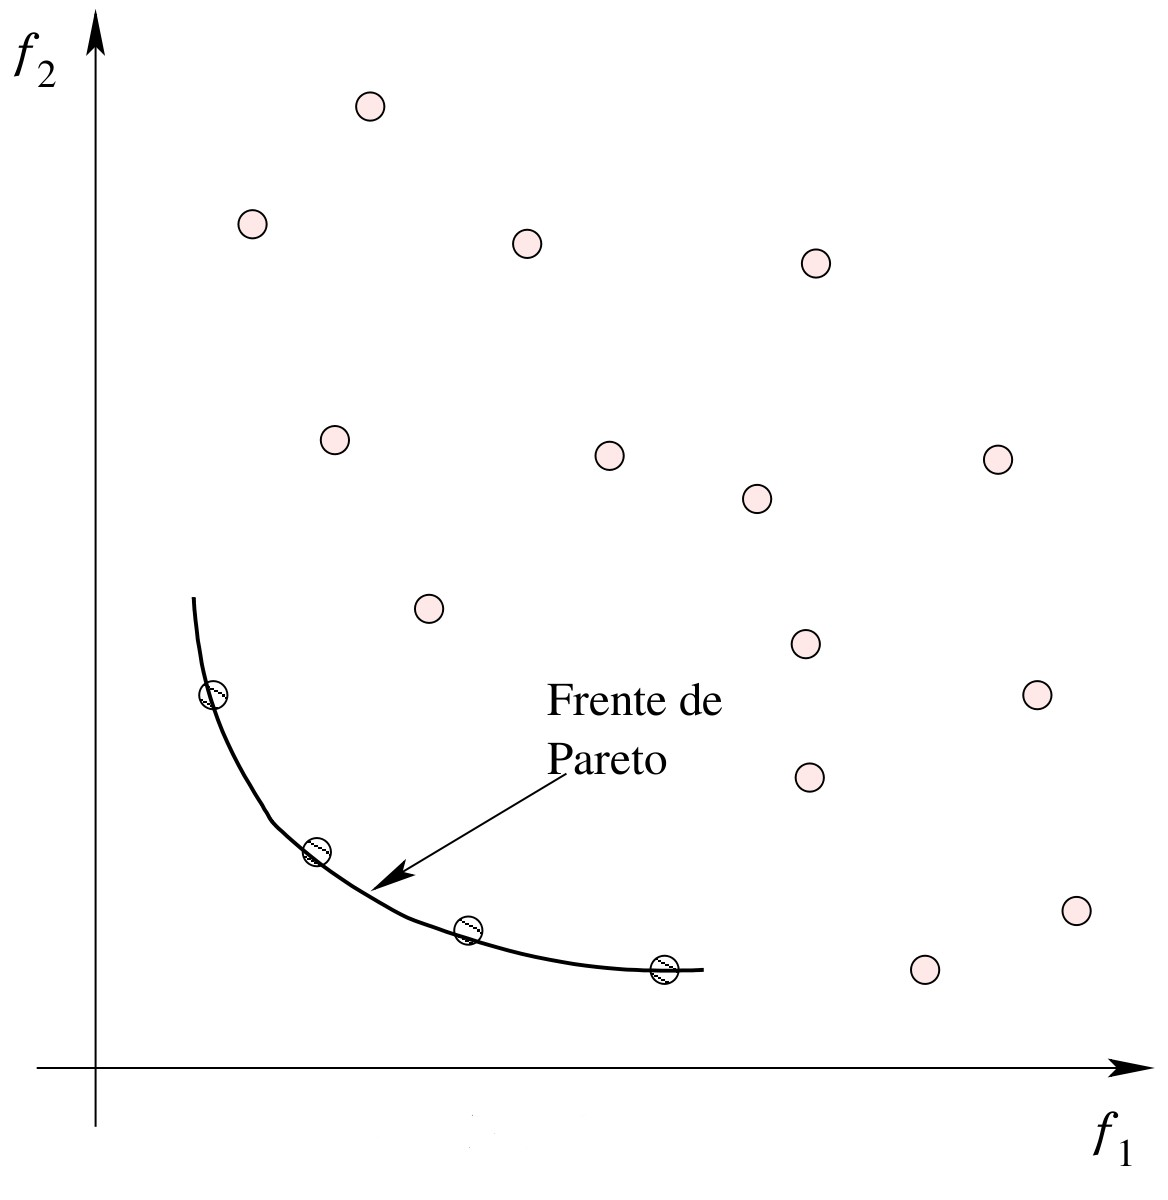
\includegraphics[keepaspectratio,width=8cm]{figuras/frentePareto.jpg}
\caption{Ejemplo de frente de Pareto con dos objetivos a minimizar.}
\label{frente}
\end{figure}

Los EAs que intentan optimizar un problema de dos o más objetivos
mediante el concepto de
optimalidad de Pareto se llaman MOEAs (\textit{Multi-Objective Evolutionary Algoritms})
\cite{Deb2004,Coello2007}, y su marco general suele ser igual que el de los EAs, es decir,
un proceso iterativo en el que evoluciona una población de individuos sujetos una serie de
operadores de selección, cruce y mutación, pero teniendo en cuenta a varias funciones
objetivo para guiar el proceso de búsqueda. Al igual que con los EAs, los MOEAs también se
pueden utilizar para el diseño de modelos de red para multiclasificación de patrones, a lo
que se le llama redes neuronales artificiales evolutivas multi-objetivo
(\textit{Multi-Objective Evolutionary Artificial Neural Networks}, MOEANNs)
\cite{Jin2006c}.

\subsection{Clasificación de MOEAs}\label{clasificacionMOEAS}
\noindent A continuación vamos a realizar una breve descripción y clasificación de los
métodos de optimización multi-objetivo más utilizados.
Concretamente, dividiremos las técnicas multi-objetivo en dos, métodos clásicos y métodos
que utilizan el concepto de óptimo de Pareto, aunque hay autores que realizan otro tipo de
clasificación. Para una revisión más completa sobre la clasificación que se muestra a
continuación ver \cite{Deb2004,Coello2007}:
\begin{description}
\item [MOEAs clásicos:] En este tipo de algoritmos no se considera el concepto
de óptimo de Pareto para la obtención de la solución final a un problema MOP, sino
que se hacen aproximaciones, no pudiéndose encontrar varias soluciones en una sola
ejecución. Por
ejemplo, estos métodos comprenden desde técnicas agregativas o con término de
regularización hasta otros métodos clásicos de
los que se hablará a continuación.
\item [MOEAs que usan el concepto de dominancia y óptimo de Pareto:] En este tipo de
algoritmos se considera el concepto de óptimo de Pareto para la obtención de la
solución final a un problema MOP, ejemplos de ellos son algoritmos como \textit{NSGAII}
\cite{Deb2002} y \textit{SPEAII} \cite{Zitzler2001}.
 \end{description}

\subsubsection{MOEAs clásicos}
\noindent Estos métodos, los cuales el lector puede consultar en
\cite{Deb2004,Coello2007}, tienden a convertir un problema multi-objetivo en otro
problema de optimización global o en un problema mono-objetivo, siendo los siguientes los métodos
más conocidos:
\begin{description}
\item [Métodos agregativos o con término de regularización:] Para
obtener la solución a un MOP basta con encontrar el mínimo o el máximo de una única
función que resume o combina todos los objetivos que se desean optimizar en uno solo. Pero
hay una serie de problemas en esta metodología. El más relevante es que se debe
proporcionar información
escalar precisa
sobre la importancia de los objetivos, a fin de evitar que uno de ellos domine a los
demás,
por lo  que  hay  que  saber  el  comportamiento  de  cada  una  de  las funciones
objetivo y tener un conocimiento “a priori” de la superficie de error. La determinación
del término de regularización adecuado para un determinado problema o factor de
aprendizaje, resulta a veces un proceso tedioso de
prueba y error. Además, solo son útiles cuando el frente de Pareto es convexo:
\begin{displaymath}
	min_{x}f_{sum}=\sum_{i=1}^k w_{i}f(\mathbf{x}) \quad x\in \Omega
\end{displaymath}
donde $\displaystyle w_{i}\geq0,\quad \sum_{i=1}^k w_{i}=1$ y $k$ el número de objetivos,
obteniéndose una sola solución en función del valor de los pesos $w_{i}$.

En el caso de ANNs en clasificación, usualmente, los objetivos a minimizar
de manera conjunta son el error
del clasificador y el número de conexiones o de nodos de los modelos de red. Así, lo que
se minimiza es el error cuadrático medio o $MSE$ (o algún otro error asociado
a la precisión del clasificador) y  se añade  un término de regularización que evite
redes
de gran tamaño. En \cite{Ludemir2006} se hace una optimización simultánea de la
estructura y los pesos de un modelo de red para generar topologías simples y con alto
porcentaje de clasificación mediante término de regularización. Los objetivos a minimizar
son la complejidad de la red y el número de patrones mal clasificados. En \cite{Jin2006b}
se estudian una serie de técnicas para trasladar la capacidad de generalización
con ANNs desde un marco multi-objetivo a uno mono-objetivo.
\item [Método de optimización minimax con pesos:] En este método se efectúa una
optimización $min-max$. Para ello se define un vector cuyos términos son las funciones
objetivo multiplicadas por diferentes pesos. El MOP se convierte en la
minimización con respecto al vector $\mathbf{x}$ del máximo valor del vector definido, para unos
pesos dados ``a priori``:
\begin{displaymath}
min\left[ max_{x\in\Omega} \left(w_{1}\cdot f_{1}(\mathbf{x}),\cdots,w_{k}\cdot
f_{k}(\mathbf{x})\right)
\right]
\end{displaymath}

Otra variación de este método se produce al fijar un vector constante que se resta al
vector de funciones objetivo, de forma que la formulación del problema queda:
\begin{displaymath}
min\left[ max_{x\in \Omega}\left(w_{1} \cdot
\left(f_{1}(\mathbf{x})-\gamma_{1}\right),\cdots,w_{k} \cdot
\left(f_{k}(\mathbf{x})-\gamma_{k}\right)\right) \right]
\end{displaymath}
\item [Método de permutación $\epsilon$:] Este método reduce un MOP a un problema
mono-objetivo con restricciones, y sirve para obtener aproximaciones en frentes convexos y
no convexos. Se basa en la minimización de una función objetivo principal y  considera  los
demás objetivos como restricciones acotadas por ciertos  niveles permisibles  $\varepsilon_{i}$
, efectuándose una minimización con un solo objetivo para la función objetivo más
relevante, sujeta a restricciones adicionales en las otras funciones objetivo:
\begin{gather} \nonumber
min_{x}f_{k}(x) \\ \nonumber
\text{sujeto a} \quad  f_{i}(x)\leq\epsilon_{i} \quad \forall i\neq k \\ \nonumber
x \in \Omega \nonumber
\end{gather}
\item [Métodos de las métricas ponderadas:] En estos métodos se considera un punto
utópico o solución ideal $f^*$, a la que se desea llegar mediante la minimización de una
función objetivo a través de una determinada métrica, como puede ser la distancia euclídea
o la métrica de \textit{Tchebycheff} \cite{Karlin1966}.
\begin{displaymath}
min \left( \sum_{i=1}^k w_{i}	\parallel f^*-f(x)\parallel^\rho\right) ^{(1/\rho)}, \quad
{x\in\Omega}
\end{displaymath}
donde $\rho$ puede tomar valores entre $\left[ 1,\infty\right]$.
\item [Programación por metas:] La idea principal de la programación por metas es
encontrar soluciones que logren un objetivo predefinido para una o más funciones
objetivo. Si la solución al objetivo predefinida no existe, el propósito es minimizar las
desviaciones de todos los objetivos.
Si consideramos una función objetivo $f(x)$, y un valor $t$ para cada objetivo de diseño,
la solución es encontrar el objetivo que alcance el valor $t$, sujeto a que debe ser una
solución factible:
\begin{displaymath}
 \text{objetivo} \quad f(x)=t, \quad x\in\Omega
\end{displaymath}
% Si el valor $t$ es más pequeño que la solución óptima $f(x^*)$ no existe solución
% factible que alcanze el objetivo exacto, por tanto se intentaría encontrar la solución
% que minimice la desviación entre el objetivo alcanzado y el deseado, $f(x^*)-t$. Si el
% valor $t$ es mayor, la solución al problema es $x$,
\item [Soluciones óptimas lexicográficas:] Este método convierte el problema de
optimización de Pareto, donde todas las componentes del vector de funciones $f(\cdot)$
tienen la misma importancia, en un problema donde las componentes de dicho vector tienen
una importancia decreciente. Así, el problema de optimización lexicográfica se formula
como una secuencia de $k$ minimizaciones $P_{i}$ de tipo:
\begin{gather} \nonumber
min_{x\in\Omega} f_{k}(x)\\ \nonumber
\text{sujeto a} \quad f_{i}(x)\leq\alpha_{i}, \quad i=1,\cdots,k-1 \nonumber
\end{gather}
\end{description}

Los métodos clásicos, generalmente, no suelen ser eficaces debido a:
\begin{enumerate}
\item Sólo dan un punto del frente de Pareto como solución, siendo
necesaria la repetición del algoritmo un gran número de veces para obtener todas las
soluciones.
\item Muchos de estos algoritmos necesitan un conocimiento previo del problema para
ser viables. Es el caso del valor de las funciones de peso o del punto utópico u óptimo.
\item Alguno de estos algoritmos son muy sensibles a la forma del frente de Pareto.
\item Estos algoritmos no son válidos en problemas con incertidumbre o en problemas
estocásticos.
\item Los algoritmos de optimización clásicos no son válidos para resolver problemas de
un sólo objetivo con un espacio de búsqueda discreto, luego tampoco lo son para resolver
MOPs con espacio de búsqueda discreto.
\end{enumerate}

\subsubsection{MOEAs que usan el concepto de dominancia y óptimo de Pareto}
\noindent Los algoritmos que utilizan el concepto de óptimo de Pareto para obtener un
conjunto de soluciones, que representan un compromiso entre los distintos objetivos a
optimizar, se pueden dividir, de forma general, en métodos no elitistas y elitistas, o
en
métodos de primera generación y de segunda generación respectivamente. Se entiende por
método elitista aquel que utiliza de una manera u otra al mejor o mejores individuos de
una población para avanzar en el proceso de evolución, mientras que los métodos no
elitistas no suelen retener las mejores soluciones de una generación a otra, o formar
conjuntos externos de mejores soluciones que sustituyan a individuos de la población en
determinados momentos de la evolución.

A continuación solo se hará referencia a los MOEAs más populares en la literatura que usan
el concepto de óptimo de Pareto, dejando al lector la
consulta de \cite{Deb2004,Coello2007} para obtener una descripción más detallada y amplia
de éstos y de otros algoritmos.
\begin{description}
	\item[Métodos no elitistas:] Estos métodos no utilizan operadores que ayuden a
preservar la elite de individuos dentro de una población, con lo que si se obtiene una
buena solución en generaciones tempranas de un EA, ésta puede que no llegue al final de
la evolución si no se realizan los procesos de selección, cruce y mutación oportunos.
Tienen la ventaja de que son fáciles de entender y sencillos de implementar, y algunos de
ellos convergen bien y encuentran un conjunto de soluciones de Pareto bien distribuidas y
diversas. Ejemplos de estos algoritmos son VEGA (\textit{Vector Evaluated Genetic
Algorithm}, MOGA (\textit{Multiple Objective Genetic Algorithm}), NSGA
(\textit{Non-Dominated Sorting Genetic Algorithm}), NPGA (\textit{Niched-Pareto Genetic
Algorithm}), HLGA (\textit{Hajela and Lins Genetic Algorithm}), MSGA (\textit{Multisexual
Genetic Algoritm}) y PESA (\textit{Pareto Envelope-based Selection Algorithm}).

\item[Métodos elitistas:] Este tipo de algoritmos usan operadores para preservar la
diversidad y los mejores individuos de una generación a otra. Por norma
general, obtienen mejores soluciones que los algoritmos de primera generación, ya que
la probabilidad de que la población de hijos mejore de una generación a otra mediante
operadores de selección, cruce y mutación adecuados es mayor (se suele
mantener una población secundaria).

Existen muchas formas de implementar el elitismo, por ejemplo,
guardando el mejor individuo de la población o cruzando padres y uniéndolos a la población
hija, escogiendo los $N$ mejores individuos. La elección del número de
individuos de elite que deben pasar de una generación a otra es importante, pues si
este número es grande disminuirá la diversidad de la población, lo que se conoce como presión
selectiva. Se podría pensar que en los algoritmos no elitistas
también se podrían conservar los mejores individuos de una generación para incluirlos en
la siguiente, pero en ese caso no estaríamos teniendo en cuenta el concepto de Pareto, y
sería difícil identificar qué soluciones son las que tienen un mejor compromiso entre los
objetivos que
perseguimos. Ejemplos de algoritmos elitistas son: NSGAII (\textit{Non-Dominated Sorting
Genetic Algorithm 2}), PAES (\textit{Pareto-Archived Evolution Strategy}), SPEA
(\textit{Strength Pareto Evolutionary Algorithm}), SPEAII (\textit{Strength
Pareto Evolutionary Algorithm 2}), PESAII (\textit{Pareto Envelope-based Selection
Algorithm 2}), $\mu \text{GA}$ (\textit{micro Genetic Algorithm}), parEGO (\textit{Pareto
Efficient Global Optimization}), $\epsilon\text{-MOEA}$ (\textit{epsilon} MOEA), MOMGA
(\textit{Multi-Objective Messy Genetic Algorithm}), PDE (\textit{Pareto Differential
Evolution}) y MOEAs con utilización de restricciones.
\end{description}

\section{Medidas $(MS,C)$ en redes neuronales artificiales}\label{objetivosRedes}
\noindent La utilización de la precisión, $C$ y la mínima sensibilidad, $MS$, en el
diseño de modelos de ANNs para problemas de clasificación multi-clase es novedoso.
%, a
%pesar de que estos dos objetivos sean subconjuntos de la superficie formada por
%los $Q(Q-1)$  puntos exteriores a la diagonal principal de la matriz de confusión.
Habitualmente lo que se pretende optimizar cuando se utilizan modelos de red para
clasificación de patrones en problemas multi-objetivo es la precisión y la complejidad de
la red \cite{Goh2008,Dehuri2009,Jin2005}, ésta última definida mediante alguna de las
siguientes formas:
\begin{description}
\item[Complejidad gaussiana o \textit{Weight Decay}:] La complejidad se define como la
suma de los pesos al cuadrado de cada una de las conexiones de la red dividido por dos.
\begin{displaymath}
\Omega(R)=\frac{1}{2}\sum_{k} W_{k}^2
\end{displaymath}
siendo $W_{k}$ el valor del peso $k$-ésimo de la red $R$. Tiene la desventaja de que no
es
capaz de llevar los pesos pequeños e irrelevantes a cero cuando se utilizan algoritmos
de	aprendizaje basados en gradiente.
\item[Complejidad de Laplace:] Es una alternativa al método anterior para llevar a
cero los pesos irrelevantes, y se define como la suma en valor absoluto de los valores de
los pesos:
\begin{displaymath}
\Omega(R)=\sum_{k} \arrowvert W_{k}\arrowvert
\end{displaymath}
\item[Número de enlaces de la red:] El número total de enlaces de una red como medida
de complejidad tiene una naturaleza discreta, por lo que es un buen
método para usarlo en optimización evolutiva, pero no es bueno aplicarlo a métodos
basados en gradiente. Se define como la suma de cada uno de los enlaces existentes en
la red:
\begin{displaymath}
\Omega(R)=\sum_{i}\sum_{j} \arrowvert lk_{ij}\arrowvert
\end{displaymath}
siendo $lk_{ij}$ el peso que va desde una neurona $i$ de la capa oculta a una neurona $j$
de la capa de entrada.
\item[Número de neuronas en la capa/s oculta/s de la red:] Similar al método anterior,
pero en esta ocasión se realiza una suma del número de neuronas que existan en la capa
o capas ocultas de una determinada red.
\begin{displaymath}
\Omega(R)=\sum_{i}\sum_{j}h_{ij}
\end{displaymath}
siendo $h_{ij}$ la neurona número $j$ de la capa oculta $i$.
\end{description}

Existen trabajos y estudios para la clasificación de patrones biclase que utilizan la
precisión y la sensibilidad como medidas de rendimiento \cite{Jin2006b},
utilizando o no ANNs. Concretamente se utiliza la maximización de la
sensibilidad o $TPR$ y la minimización del $FPR$, o de otra manera, $TPR$ y $Sp$
$\left(1-FPR\right)$, como objetivos a maximizar. En \cite{AlbertoF2009}, la métrica
seleccionada es la media geométrica de los porcentajes positivos, midiendo de esta manera
un rendimiento más balanceado que usando solamente la precisión global. Pero el
concepto de sensibilidad que se usa en la mayoría de este tipo de trabajos solo sirve para
problemas binarios y no para multiclase.

\section{Trabajos con MOEANNs}
\noindent Tradicionalmente, como acabamos de comentar, en el diseño de ANNs mediante MOEAs
se suelen establecer dos objetivos a optimizar, el error en entrenamiento y la complejidad
de la red. Por ejemplo, Abbass \cite{Abbass2001,Abbass2003}, el principal exponente en
este aspecto, ha presentado diferentes estudios sobre el diseño y entrenamiento de ANNs
para clasificación y regresión, usando precisión y complejidad como objetivos en MOEAs.
Abbass establece un marco general para evolución multi-objetivo de ANNs basado en
DE (\textit{Differential Evolution}) \cite{Price2005} (ver capítulo \ref{diferencial}), donde se
evoluciona conjuntamente, para cada red, la estructura y los pesos, y se aplican operadores de cruce
y mutación, basados en la selección aleatoria (sin repetición) de tres padres de la población.

En cuanto a aplicaciones de MOEAS para el entrenamiento de ANNs cabe destacar el
reconocimiento de imágenes propuesto en \cite{Wiegand2004}, donde se detectan y clasifican rostros
humanos mediante MOEANNs usando el algoritmo NSGAII e introduciendo una LS en cada generación de
la evolución. Los objetivos a optimizar son el $MSE$ y el número de neuronas en capa
oculta. Algunos artículos y variaciones encaminadas en la misma dirección que el citado
trabajo se pueden consultar en \cite{Roth2006,Gepperth2006}.

Yauchu Jin, en varios de sus artículos \cite{Jin2004,Jin2005,Jin2006} hace un estudio de
los resultados obtenidos con el algoritmo NSGAII, comparándolo con otros MOEAs y con
algoritmos mono-objetivo con término de regularización para ANNs. Se usan como objetivos la
minimización del $MSE$ y la complejidad de la red, y también emplea versiones híbridas con
algoritmos de LS como el \textit{Resilient Backpropagation} (Rprop) \cite{Riedmiller1993}.

En \cite{Jin2006b} se pueden estudiar algunas técnicas y heurísticas para obtener el
frente de Pareto. Se basan no solo en entrenar redes aplicando el conjunto de
entrenamiento a modelos de red a lo largo del proceso evolutivo, para finalmente
aplicar el conjunto de generalización, sino que se basan también en determinados ajustes
sobre los datos de entrenamiento, como por ejemplo: la adición de ruido gaussiano, que
consiste en la adición a los datos del conjunto de entrenamiento de un ruido
gaussiano cada cierto número de generaciones, o la adición de ruido a través de
medias, que consiste en la adición a los datos del conjunto de entrenamiento de un
ruido partiendo de valor medio de cada entrada.

Otros trabajos \cite{Fieldsend2002,Fieldsend2005} utilizan otras técnicas sobre los
conjuntos de entrenamiento para mejorar la capacidad de generalización cuando se obtiene
el frente de
Pareto, proponiendo un determinado MOEA, dependiendo de si en la obtención del frente se
utiliza: a) el conjunto de entrenamiento, b) los conjuntos de entrenamiento y validación
o c) el conjunto de entrenamiento con técnicas de \textit{bootstraping} (muestreo con
reemplazamiento) \cite{Bootstrapping2006} para prevenir el
sobre ajuste en entrenamiento.

Otros autores como M. Delgado y colaboradores, utilizan modelos de clasificación utilizando ANNs
recurrentes para el entrenamiento y obtención de modelos de red. Así, en
\cite{Delgado2005} se utiliza una
mejora del algoritmo SPEA en problemas de inferencia gramatical, donde se optimizan tres
objetivos: maximizar el número de aprendizajes positivos en entrenamiento, minimizar el
error cometido, y minimizar el número de neuronas en la red. La codificación es directa,
empleando cruce y mutación para la obtención de nuevos hijos. En \cite{Delgado2007} se
utilizan redes recurrentes dinámicas con una versión híbrida de SPEAII, intentando
minimizar el $MSE$ y el número de neuronas en capa oculta, utilizando un algoritmo de LS
basado en gradiente. Como operadores se utiliza tanto cruce como mutación.

En \cite{Gonzalez2003} se aplican varios operadores de cruce y mutación basados en las
transformaciones de matrices SVD (\textit{Singular Value Descomposition}) y OLS
(\textit{Orthogonal Least Squares}), que producen modificaciones locales y globales en
redes RBF. Los objetivos a optimizar
son el $MSE$ y la complejidad de la red, utilizando el procedimiento de orden
del algoritmo MOGA y aplicándole el método de Levenverg-Maquart \cite{Marquardt1963} como
algoritmo de LS. Un criterio parecido se utiliza en \cite{Hatanaka2006}, pero en este caso
el MOEA aplicado es NSGAII.

En \cite{Yen2006} se propone una forma de asignación de aptitud basada en la densidad de
orden en un algoritmo llamado HRDGA (\textit{Hieralchical Rank Density Genetic
Algorithm}). Se convierten múltiples objetivos de alta dimensionalidad en dos, complejidad
de la red y error cometido, minimizando el error de orden de un individuo en concreto y el
valor de densidad de la población. Los individuos del frente de Pareto se buscan por medio
de esquemas de difusión y elitismo, y se previene la introducción de individuos dañados
mediante el concepto de región perdida.

Existe otro buen número de trabajos relacionados con MOEAs para el entrenamiento de ANNs,
pero entendemos que este no es el objetivo principal de este trabajo de tesis. El lector
puede consultar un estado del arte más amplio en \cite{Ou2007,Goh2008,Jin2008}.

Abordamos a continuación el algoritmo MPENSGAII, como propuesta fundamental y uno de los
objetivos de este trabajo de tesis.

\section{El algoritmo MPENSGAII}\label{algoritmo}
\noindent A partir de ahora se utilizarán términos y se hará referencia a
metodologías y expresiones formales explicadas y detalladas en los capítulos
\ref{medidasRendimiento} y \ref{redesneuronales}
de esta tesis. En esta sección exponemos  MPENSGAII (\textit{Memetic Pareto
NSGAII}) \cite{Fernandez2010}, un MOEA para la obtención de modelos de ANNs para
multi-clasificación de patrones, utilizando como modelo funcional unidades de base
sigmoides (SUs), ya introducidas en la sección \ref{unidadesSigmoide} del
capítulo \ref{redesneuronales}, y usando un algoritmo de LS para mejorar la capacidad de
generalización de los multiclasificadores y el proceso de aprendizaje.

MPENSGAII se basa en NSGAII \cite{Deb2002}, utilizando como características más
representativas el ordenamiento rápido de no-dominados para la obtención
del frente de Pareto, el cálculo de la distancia \textit{crowding} para el mantenimiento
de la diversidad, y la selección por torneo binario. En esta sección no explicaremos este
tipo de operadores y técnicas al considerarlo repetitivo, ya que siguen la misma filosofía
usada en NSGAII, dejando al lector una descripción detallada sobre ello en \cite{Deb2002}.

MPENSGAII obtiene diferentes conjuntos de clasificadores
no dominados que presentan un buen balanceo entre $C$ y $MS$ (ver capítulo
\ref{medidasRendimiento}), que son los dos objetivos a optimizar. El
ordenamiento rápido de no dominados utiliza como medidas para determinar la no dominancia
de un individuo, dos funciones objetivo que miden la precisión del mismo, y que se
detallan en la siguiente sección.

MPENSGAII estima los parámetros y la estructura de la red de manera simultanea. La
población de individuos está sujeta a operaciones de replicación y de mutación, no
usando operador de cruce, por las mismas razones que en el algoritmo CBFEP del capítulo
\ref{evoMonoObjetivo}. En cuanto a la codificación de los modelos de red, se sigue la
misma codificación explicada en el algoritmo CBFEP, pero aplicado solo a ANNs con SUs, en
vez de a modelos híbridos.

\subsection{Funciones objetivo}\label{funcionesObjetivo}
%Aqui iba lo primero que he puesto en trabajos previos con MOEANNS
\noindent Si asumimos que todos los errores de clasificación son igualmente costosos y que
no hay preferencia ni penalización para una determinada clase de patrones, un buen
clasificador debería obtener un alto nivel de precisión global, así como un
aceptable nivel de clasificación para cada clase de un problema. En
problemas reales, estos objetivos suelen estar en conflicto (ver sección \ref{propiedades}
del capítulo \ref{medidasRendimiento}), por tanto la aplicación de un MOEA para la
resolución de este problema es una buena opción. Teniendo en cuesta ésto, las dos
funciones objetivo a optimizar con MPENSGAII son:
\begin{itemize}
\item La mínima sensibilidad de todas las clases del problema, $MS$:
\begin{displaymath}
A_{1}\left( g,\mathbf{\Theta}\right) = MS(g)
\end{displaymath}
\item La entropía cruzada, $E$, como medida de error global, (al igual que con el algoritmo
CBFEP), ya que aunque depende del conjunto de datos, se ha demostrado que, por norma
general, $E$ converge mejor que $C$ (ver sección \ref{etapas} del capítulo
\ref{evoMonoObjetivo}). Concretamente, como función de aptitud a la hora de
evaluar un individuo se usará la siguiente expresión:
\begin{displaymath}
\label{aptitudNNEP}
A_{2}\left( g,\mathbf{\Theta}\right) =\frac{1}{1+E\left( g,\mathbf{\Theta}\right)}
\end{displaymath}
es decir, maximizar una transformación estrictamente decreciente de $E$.
\end{itemize}

Para asignar una clase a una nueva observación se sigue el esquema ``1 de $Q$''
explicado en el algoritmo CBFEP.

En \cite{Fernandez2009a} se puede estudiar una variante de MPENSGAII en la que
utilizamos los siguientes objetivos:
\begin{itemize}
\item Minimizar el coeficiente de variación de las sensibilidades (\textit{Variation
Coefficient}, VC):
\begin{displaymath}
A_{1}=VC=\frac{\sqrt{\frac{\sum_{i=1}^{Q}(S_{i}-\bar{S})^2}{Q-1}}}{\bar{S}}
\end{displaymath}
siendo $\bar{S}$ la media de las sensibilidades de cada clase $S_{i}$.
\item Como segunda función objetivo emplea $E$, es decir, la función
objetivo $A_{2}$ de MPENSGAII.
\end{itemize}

En esta variante comparamos con algoritmos, como el algoritmo MPANN \cite{Abbass2003} y
con un
evolutivo en dos etapas llamado E+A \cite{Martinez-Estudillo2008} (ver sección \ref{balanceados} del
capítulo \ref{medidasRendimiento}), presentando buenos resultados en una serie conjuntos de datos
obtenidos de la UCI \cite{UCI2007}. La metodología seguida es similar a la de MPENSGAII,
pero solo cogiendo la parte superior del frente de Pareto, la que proporciona el mejor
individuo en $E$, y no los dos extremos como veremos en las siguientes secciones.
Esto nos permitió poder comparar con los algoritmos antes mencionados.
\newpage
\subsection{Operadores}\label{operadoresMPENSGAII}
\noindent Los operadores utilizados  en cuanto a mutación son prácticamente los mismos que
los utilizados con CBFEP.

Hay 4 mutaciones estructurales: Añadir neurona, AN, eliminar neurona,
DN, añadir enlace, AL y eliminar enlace, DL. Se realizan de la misma forma que con el
algoritmo CBFEP, pero en este caso, al utilizar solo SUs como unidades de base, no es
necesario elegir el tipo de unidad a introducir en capa oculta.

La mutación paramétrica sí cambia con respecto CBFEP, puesto que se aplica a cada uno de
los pesos de la red, añadiéndoles un ruido gaussiano dado por:
\begin{gather} \nonumber
w_{ij}(t+1) = w_{ij}(t)+\xi_{1}(t)\\ \nonumber
\theta_j(t+1) = \theta_{j}(t)+\xi_{2}(t)\\ \nonumber
\beta_{ij}(t+1) = \beta_{ij}(t)+\xi_{3}(t) \nonumber
\end{gather}
donde $\xi_{1}(t)$, $\xi_{2}(t)$ y $\xi_{3}(t)$ son variables aleatorias normales
$N(0,T(t))$, donde $T(t)$ representa la temperatura en la generación $t$ a lo largo de la
evolución (el valor de $T(t)$ disminuye produciéndose descensos más drásticos al comienzo
de la evolución (exploración), y más lentos al final (explotación). La temperatura $T$ en
en la generación $t$ viene dada por:
\[
T(t)=
\begin{cases}
r \cdot T(t-1) & \text{ si } t=kI,k=1,2,\cdots,\frac{I_{max}}{I_{t}}\\
T(t) & \text{en los restantes casos}
\end{cases}
\]
donde $r$ es el factor de descenso, $I_{t}$ el número de
generaciones que deben transcurrir para que se actualice el valor de la temperatura e, $I_{max}$ es
el número máximo de generaciones que se ejecutará MPENSGAII.

A cada individuo de la población se le aplica aleatoriamente una y solo una de las 5
mutaciones utilizadas. Si alguna mutación no tiene éxito por alguna restricción especial
referida a la arquitectura de la red (ver mutaciones del algoritmo CBFEP), se
elige otra mutación aleatoriamente.

Las mutaciones AL y DL se aplican solamente en capa oculta y capa de salida, mientras que
las mutaciones AN y DN se realizan en capa oculta. El número de neuronas a añadir o
eliminar se elije aleatoriamente entre los valores $\left[1,2\right] $, mientras que el
número de enlaces a añadir o eliminar depende de los que haya en ese momento en cada red.
Se añadirán o eliminan el 30\% del total de enlaces que haya entre capa de entrada y capa
oculta y el 5\% del total de los enlaces existentes entre capa oculta y capa de salida.
Con respecto al valor de los pesos que se añaden en los enlaces, se toman valores entre
$\left[-5,5\right] $ para la capa entrada-oculta y $\left[ -10,10\right] $ para la capa
oculta-salida.

\subsection{iRprop+ como búsqueda local}\label{rprop}
\noindent Una mejora dentro de los EAs, tanto para algoritmos mono-objetivo como
multi-objetivo, es la incorporación de procedimientos de LS a través de la evolución
\cite{Cotta2001,Grosan2007,Goh2009}. Algunos estudios llevados a cabo sobre el proceso de
convergencia de un EA, muestran como éste encuentra rápidamente soluciones aceptables a un
problema, sin embargo y por regla general, se necesitan más generaciones para alcanzar una
buena solución \cite{Houck1997} que si se utiliza un algoritmo basado en gradiente. Por
otro lado, los algoritmos de LS pueden quedar atrapados en un óptimo local, aunque en
ocasiones pueden encontrar el óptimo global cuando la búsqueda se lleva a cabo en pequeñas
regiones del espacio. De esta forma, en combinación con EAs, los algoritmos de LS
proporcionan un método para obtener de manera rápida y eficiente buenas soluciones
a un problema \cite{Smith2007}.

Una vez dicho esto, MPENSGAII se ha mejorado mediante la implementación de un algoritmo de
LS adaptado a nuestra codificación y a nuestras funciones objetivo, concretamente el
algoritmo iRprop+ (\textit{Improved Resilient Back-propagation}) \cite{Igel2003}, que es
una mejora del original Rprop \cite{Riedmiller1993}. El algoritmo Rprop (\textit{Resilient
Back-propagation}) \cite{Riedmiller1993}, como método de LS, es una de las mejores
técnicas conocidas en este aspecto en términos de velocidad de convergencia, precisión y
robustez con respecto a sus parámetros. iRprop+ es un procedimiento basado
en gradiente, difiriendo de las técnicas clásicas de propagación hacia atrás del error en
que, las derivadas parciales de la función error, sólo se usan para determinar el
sentido en que se deben corregir los pesos de la red, pero no las magnitudes de los
ajustes. El modelo de actualización de cada peso $ij$ de una ANN viene dado por
$\displaystyle
w_{ij}^{(t+1)}=w_{ij}^{(t+1)}+\bigtriangleup w_{ij}^{(t+1)}$, donde
$\bigtriangleup w_{ij}^{(t+1)}$ se estima con una función de cambio de signo de la
derivada del error entre las iteraciones $(t)$ y $(t-1)$, y en función del tamaño de paso
para los pesos $\bigtriangleup _{ij}$, tal como se realiza tradicionalmente con las
técnicas basadas en
gradiente. Así, si el signo de la derivada no cambia en las dos últimas iteraciones, el
tamaño de paso se aumenta. Si la derivada es cero no se modifica y si cambia de signo
se disminuye. iRprop+ aplica una estrategia de \textit{backtracking} para decidir la
dirección de corrección del valor de los pesos de la red, concretamente la idea es que la
actualización de los pesos depende de la evolución del error. De esta manera, el esquema
de entrenamiento combina información local con información global (por ejemplo, el valor
del error en cada iteración) a la hora de decidir si debe modificar los pesos. Un cambio
de signo en una derivada parcial significa que se ha saltado un mínimo local. Se ha
demostrado mediante problemas de prueba o \textit{benchmarks} \cite{Igel2003}, que
iRprop+ consigue mayor rendimiento que su versión original.

En este trabajo usamos iRprop+ cuando combinamos la población de padres
e hijos en
MPENSGAII (paso 8-d de la figura \ref{marcoMPENSGAII}). Entonces, solo los individuos del
primer frente de Pareto (obtenido mediante una ordenación rápida de los individuos no
dominados) de
la población combinada se optimizan mediante el algoritmo iRprop+. El coste
computacional
asociado a este tipo de operaciones se reduce considerablemente en nuestro MPENSGAII, ya
que no aplicamos la LS a todos los individuos mutados de la población de
descendientes, ni en todas las generaciones. El procedimiento de LS se aplica sólo al
principio (2/7 del número total de generaciones), en la mitad del proceso evolutivo (4/7)
y al final (6/7) del mismo; mientras que en otros trabajos \cite{Jin2008} se usa la
LS en cada generación, y en la mayoría de las ocasiones a todos los
individuos de la población.

iRprop+ solo se ha aplicado en una dirección de las dos funciones objetivo, ya que $MS$,
en general, no es derivable. Concretamente se ha aplicado en la dirección de $E$. Así,
hemos llevado a cabo una adaptación del algoritmo a la función de activación
\textit{softmax} y a la función de
entropía cruzada, $E$ (normalmente, en la literatura específica, iRprop+ se ha utilizado con el
$MSE$), de forma que el vector
gradiente viene dado por:
\begin{gather} \nonumber
\bigtriangledown E(\mathbf{\beta}^q , \mathbf{w})=\left( \frac{\partial
E}{\partial{\mathbf{\beta}^q}},\frac{\partial E}{ \mathbf{w} }\right)
\end{gather}
donde $\mathbf{\beta}^q,\mathbf{w}$ son los vectores de parámetros asociados a una red
neuronal.

Sea $\Theta_{q}$ cualquiera de los parámetros de $\mathbf{\beta}^q$ y $\mathbf{w}$,
entonces
\begin{gather} \nonumber
\frac{\partial E}{\partial \mathbf{\Theta}_{q}}=\frac{1}{N}\sum_{n=1}^N \sum_{q=1}^Q
y_{n}^q \frac{1}{g_{q}\left( \mathbf{x}_{n},\Theta_{q}\right)}  \frac{\partial g_{q}
\left(\mathbf{x}_{n} ,\mathbf{\Theta}_{q}\right)} {\partial \mathbf{\Theta}_{q}}
\end{gather}

\begin{small}
\begin{gather} \nonumber
\frac{\partial g_{q}
\left(\mathbf{x}_{n} ,\mathbf{\Theta}_{q}\right)} {\partial \mathbf{\Theta}_{q}} =
\frac{1}{\left( 1+\sum_{q=1}^{Q-1} e ^{f_{q}}\right)^2}\left\lbrace e ^{f_{q}}
\frac{\partial f_{q}}{\partial \mathbf{\Theta}_{q}}\left(1+\sum_{q=1}^{Q-1} e
^{f_{q}}\right)-e^{f_{q}}\sum_{q=1}^{Q-1} e^{f_{q}} \frac{\partial f_{q}}{\partial
\mathbf{\Theta}_{q}} \right\rbrace
\end{gather}
\end{small}

\begin{gather} \nonumber
\frac{\partial g_{q}\left(\mathbf{x}_{n} ,\mathbf{\Theta}_{q}\right)} {\partial
\mathbf{\Theta}_{q}} = g_{q}\frac{\partial f_{q}}{\partial\mathbf{\Theta}_{q}} - g_{q}^2
e^{-f_{q}} \sum_{q=1}^{Q-1} e^{f_{q}} \frac{\partial
f_{q}}{\partial\mathbf{\Theta}_{q}}
\end{gather}

Finalmente, para la capa de salida de cada ANN se tiene que
\begin{equation*}
	\frac{\partial f_{q}}{\partial \beta_{0}^k}=\delta_{kq}=
	\begin{cases}
		0 & k\neq q \\
		1 & k=q
	\end{cases}, \quad
	\frac{\partial f_{q}}{\partial \beta_{s}^k}=
	\begin{cases}
	0 & q\neq k \\
	\mathbf{\sigma}\left( \sum_{i=1}^k w_{is}x_{i}\right)  & q=k
	\end{cases}
\end{equation*}

y para la capa de salida que
\begin{displaymath}
\frac{\partial f_{q}}{\partial w_{s}^t} = \mathbf{\beta}_{s}^q \mathbf{\sigma}'\left(
\sum_{i=1}^k w_{is}x_{i}\right) x_{t},\quad \text{donde} \quad
s=1,2,\cdots,m;t=1,2,\cdots,k
\end{displaymath}

En un trabajo futuro, quedaría abierta la opción de aplicar un algoritmo de LS en las dos
direcciones u objetivos que guían a MPENSGAII (ver artículos
de Moller \cite{Moller1993,Falas2005}), por ejemplo mediante el uso de otra función
objetivo que sustituya a $MS$ y que sea derivable, mediante un procedimiento por etapas en
las que de forma alternada o secuencial se optimicen los objetivos del problema, o
mediante algún tipo de combinación que utilice información de los dos objetivos.

\subsection{Etapas y aspectos relevantes de MPENSGAII}\label{etapas}
\noindent Una vez descritos los operadores de mutación a aplicar, los objetivos a
optimizar, y el método de LS, pasamos a comentar los aspectos más relevantes del algoritmo
MPENSGAII. El marco general de MPENSGAII se muestra en la figura \ref{marcoMPENSGAII}, y
un esquema de las etapas o pasos de MPENSGAII se encuentra en la figura
\ref{etapasMPENSGAII}.

\begin{figure}[!htp]
\centering
\fbox{
	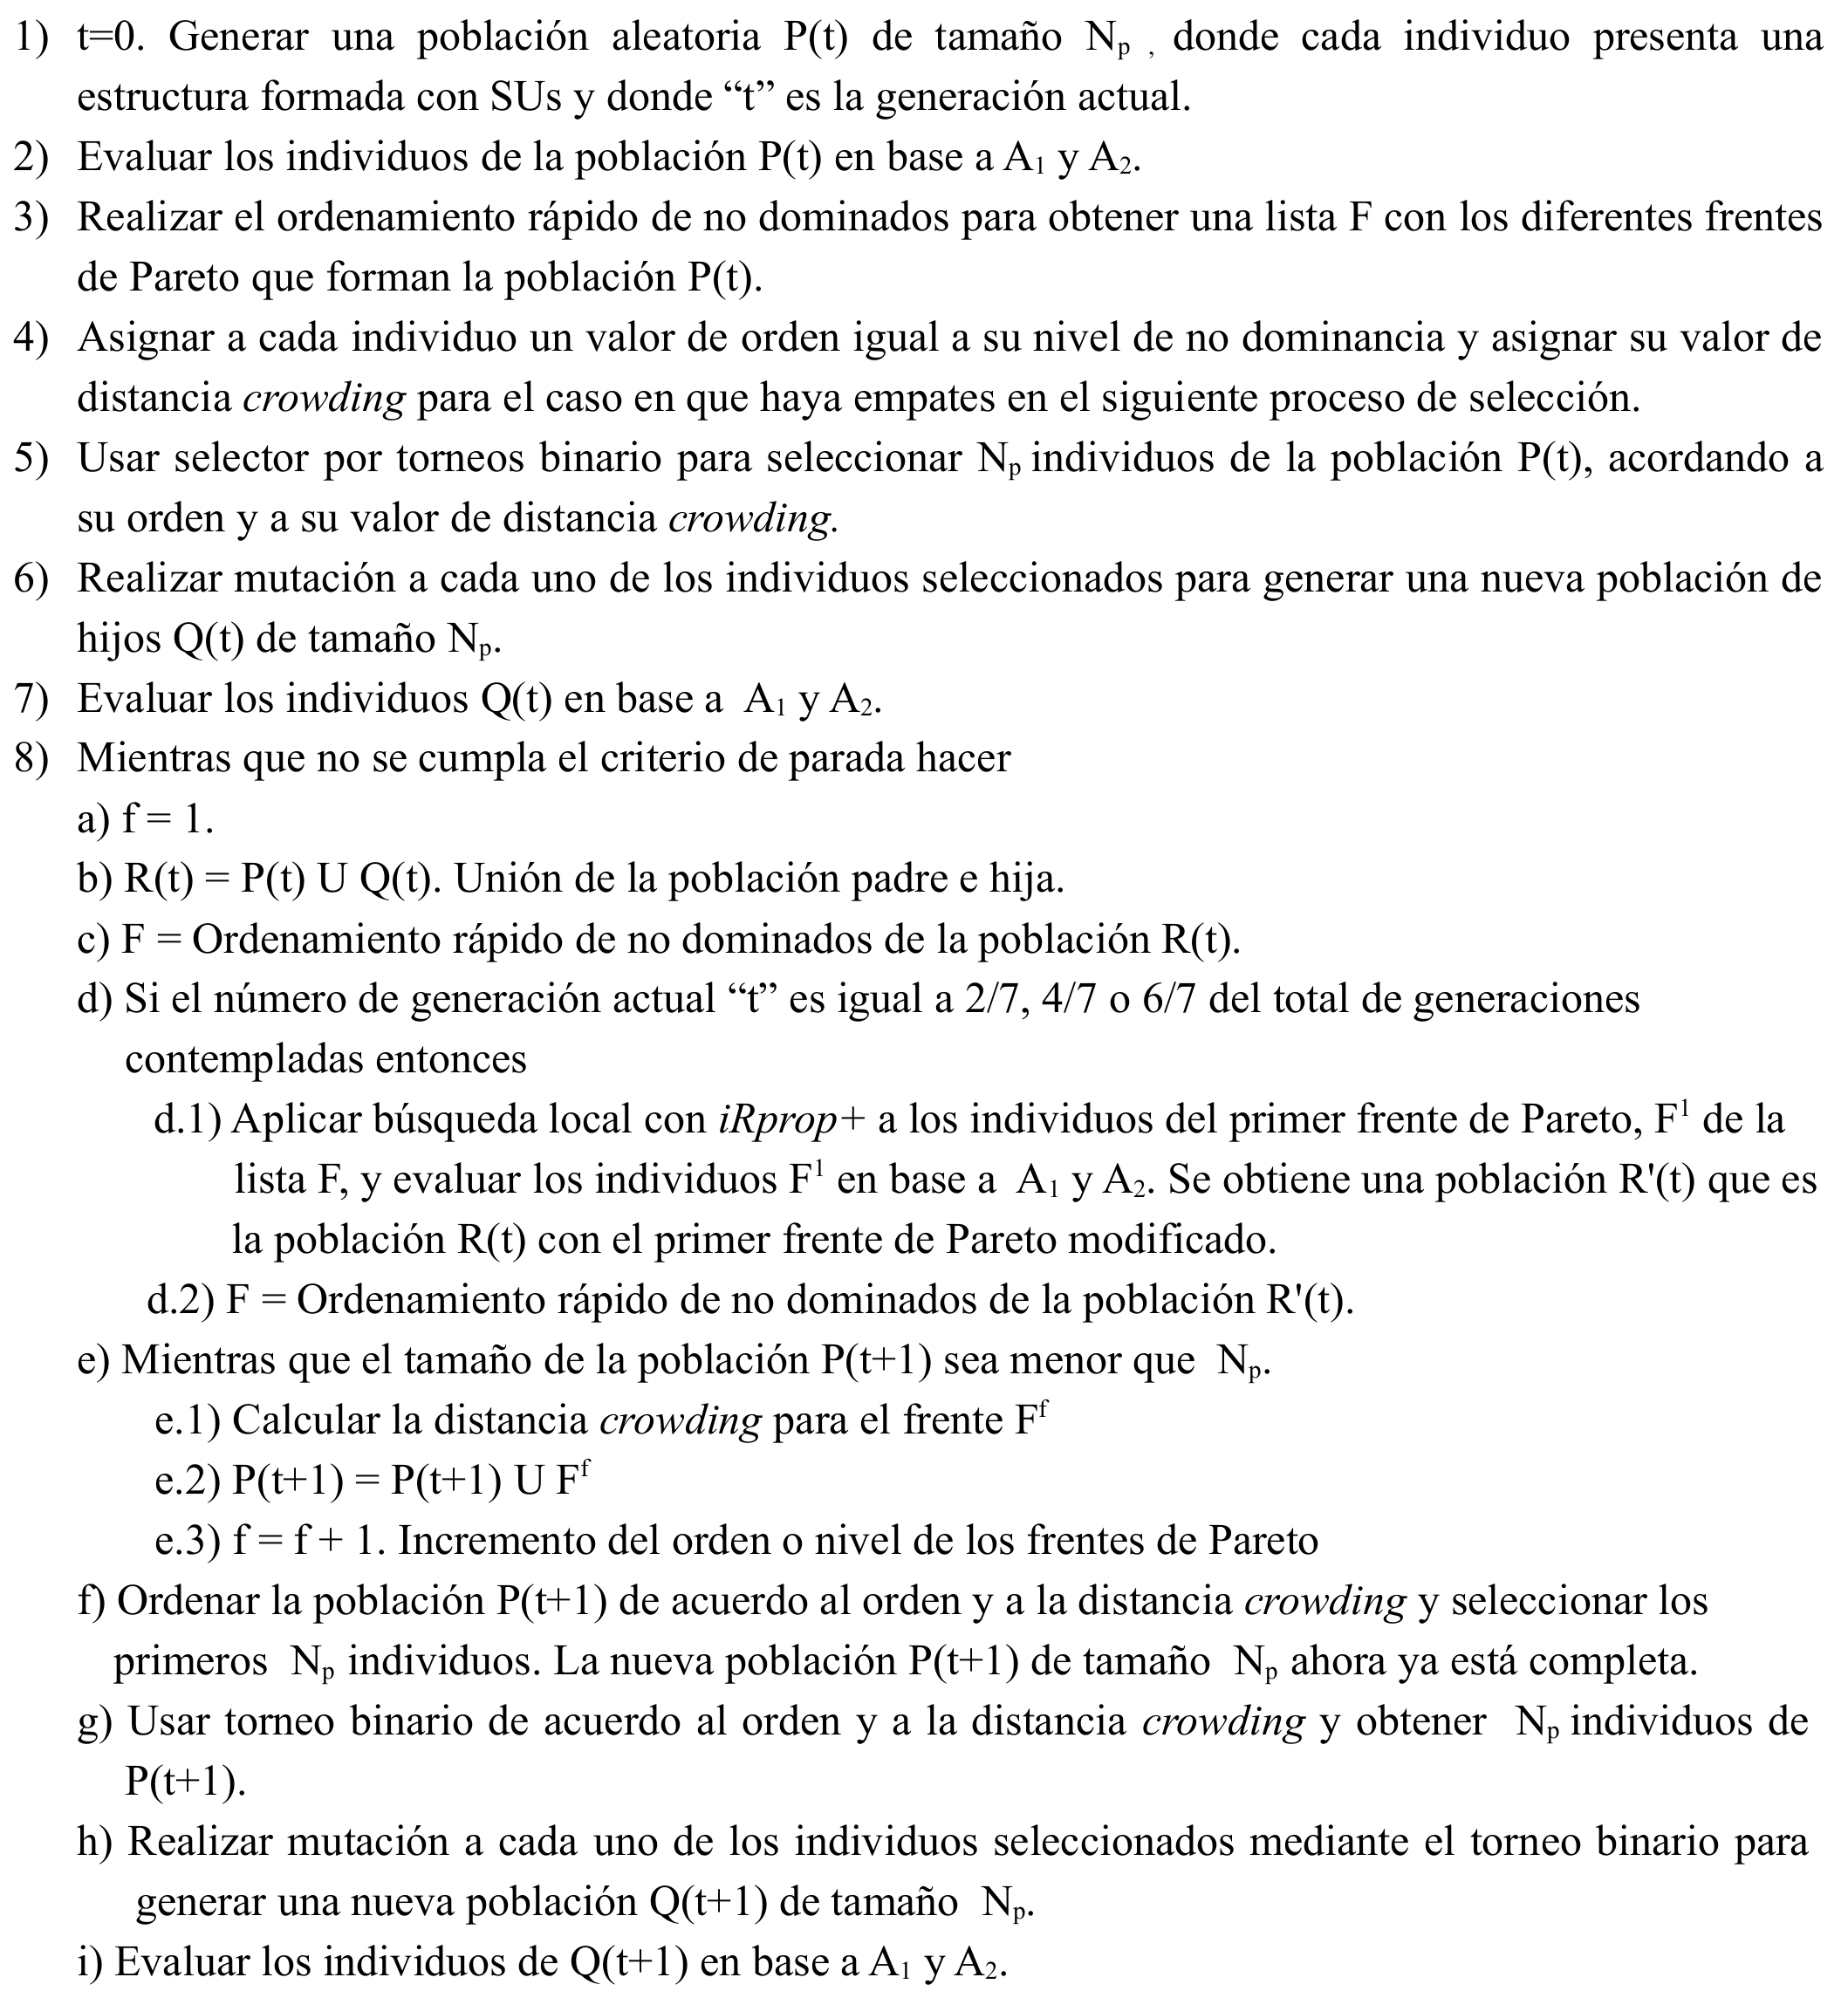
\includegraphics[keepaspectratio,width=12.5cm]{figuras/marcoMPENSGAII.jpg}
}
\caption{Pseudocódigo del marco general de MPENSGAII.}
\label{marcoMPENSGAII}
\end{figure}

\newpage

 \begin{figure}[!htp]
\centering
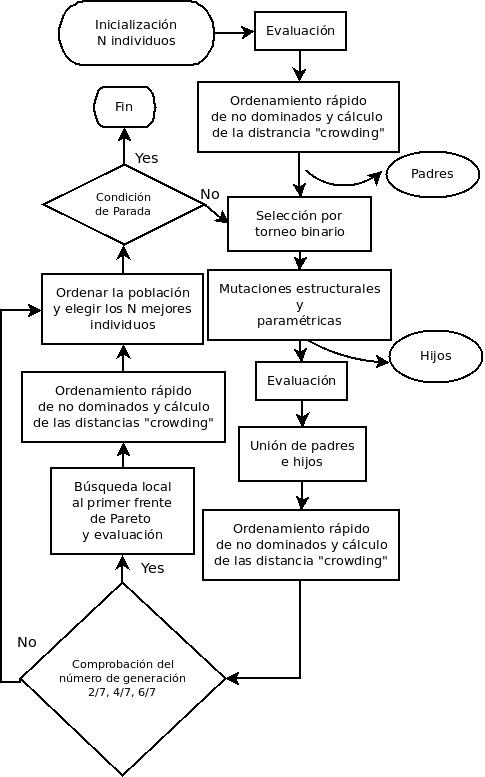
\includegraphics[keepaspectratio,width=8cm]{figuras/etapasMPENSGAII.jpg}
\caption{Etapas del algoritmo MPENSGAII.}
\label{etapasMPENSGAII}
\end{figure}

MPENSGAII comienza con la generación aleatoria de 100 ANNs con unidades de base de tipo
SU, es decir, el valor
de $N_{p}$ del paso 1 de la figura \ref{marcoMPENSGAII} es $N_{p}=100$. El valor de los
pesos asociados a los enlaces es un número aleatorio perteneciente al intervalo $\left[
-5,5\right] $ para los pesos de capa entrada-capa oculta y al intervalo $\left[
-10,10\right] $ para los pesos de capa
oculta-capa de salida. El número de neuronas en capa oculta se obtiene de la misma forma
que en el algoritmo CBFEP de capítulo anterior, es decir, considerando los parámetros
$m$, $M_{E}$ y $M_{I}$ (ver sección \ref{etapas} del capítulo \ref{evoMonoObjetivo}).

Una vez generada la población inicial, ésta se evalúa en base a
$A_{1}$ y $A_{2}$ (paso 2). Como tercer paso se hace el ordenamiento rápido de no
dominados, obteniendo una lista de frentes de Pareto. Una vez hecho esto, a cada individuo
se le asigna un valor de orden dependiendo del valor de no dominancia obtenido
en el paso anterior (1 para los individuos del primer frente, 2 para los del segundo,
...). También se asigna el valor de la distancia \textit{crowding}. Para ver con más
detalle como se realizan este tipo de operaciones consultar el algoritmo NSGAII
en \cite{Deb2002}.

Se pasa entonces a la etapa de selección de individuos. Ésta se realiza mediante un
torneo binario, de manera que se seleccionan $N_{p}$ individuos (paso 5). A los
individuos seleccionados se les aplica un operador de mutación y se etiquetan como una
nueva población (paso 6), aparte de la población inicial. Esta nueva población se evalúa
de la misma manera que en el paso 2. Una vez se tienen las dos poblaciones, comienza el
proceso evolutivo.

Primero se unen la población padre o inicial y la hija creada en los pasos anteriores,
formándose una población $R(t)$ (paso 8-b). A $R(t)$ se le aplica un ordenamiento rápido
de no dominados (paso 8-c) obteniendo una nueva lista de frentes. En este momento, si la
generación actual $t$ es igual a 2/7, 4/7 o 6/7 del total de generaciones del proceso
evolutivo, se pasa al proceso de LS. Concretamente se aplica iRprop+ al primer
frente de Pareto de la población  $R(t)$, y se evalúan los individuos. Se tiene por tanto
una población $R'(t)$  con los individuos del primer frente modificados. A $R'(t)$ se le
aplica de nuevo un ordenamiento rápido de no dominados.

Se haya utilizado o no la LS, a continuación se irá creando una
población $P(t+1)$ para la siguiente generación, de manera que ésta se genera
añadiendo individuos de la lista de frentes obtenida (paso 8-d.2) y en base a las
distancias \textit{crowding} de los individuos, hasta que el tamaño de $P(t+1)$ sea igual
o mayor a $N_{p}$ (paso e).

Cuando la población $P(t+1)$ está completa se ordena en base al orden de frente y a la
distancia \textit{crowding} y se seleccionan los primeros $N_{p}$ individuos. Entonces, la nueva
población $P(t+1)$ queda completa (paso f).

Pasamos de nuevo a realizar un proceso de selección por torneo binario, obteniendo  $N_{p}$
individuos de $P(t+1)$ (paso g).

A los individuos seleccionados se les aplica un operador de mutación, de manera que la
población $P(t+1)$ pasa a llamarse $Q(t+1)$ (paso h).

La población $Q(t+1)$ es evaluada, quedando preparada para iniciar la siguiente
generación del proceso evolutivo (paso i), el cual termina cuando se haya alcanzado el
número de generaciones indicadas al inicio del algoritmo, y que depende de cada base de
datos o problema.

\subsection{Diseño experimental} \label{disenio}
\noindent Para analizar el rendimiento de MPENSGAII hemos utilizado 17
conjuntos de datos del repositorio de la UCI \cite{UCI2007}, más otro interesante
conjunto que no pertenece a dicho repositorio, que se denomina BTX.

BTX (ver \cite{Hervas2008}) es un problema de clasificación que
consiste en discriminar entre diferentes tipos de
aguas contaminadas. El conjunto de datos  incluye un conjunto de 63 ejemplos de diferentes
aguas con
una determinada cantidad de Benceno, Tolueno y Xyleno, en concentraciones que se encuentran
entre los 5 y los 30 $\mu g/l$. Hay siete tipos de aguas contaminadas con el mismo número
de patrones por clase.

En la tabla \ref{tabla1MPENSGAII} se muestran las características de cada
conjunto de datos. La tabla está dividida en problemas binarios y problemas multi-clase.
Estos últimos, en general, son más difíciles de clasificar, ya que al aumentar
el número de clases, el valor de $p^*$ es más pequeño, y el rango de valores de $MS$ será
más amplio para valores altos de $C$ (ver sección \ref{propiedades} y \ref{balanceados}
del
capítulo \ref{medidasRendimiento}). La tabla muestra el número total de patrones por cada
conjunto de datos, el número de patrones en el conjunto de entrenamiento y en el
conjunto de generalización, el número de
variables de entrada, el número de clases, el número total de patrones por clase y el
valor de $p^*$.

El diseño experimental consiste en una partición estratificada del conjunto de datos con $3n/4$
patrones para
el conjunto de entrenamiento y $n/4$ patrones para el conjunto de generalización, siendo $n$ el
tamaño del conjunto.

%(PREGUNTAR COMO CENTRAR EL ENCABEZADO DE LA PENULTIMA COLUMNA)
\begin{table}[htb!]
\scriptsize
\caption{Características de los conjuntos de datos de la UCI y del conjunto BTX.}
\label{tabla1MPENSGAII}
\centering
\tabcolsep 1pt
\begin{tabular}{c c c c c c p{2.5cm} c}
\hline
\rowcolor[rgb]{0.70,0.85,1}\textbf{\textit{Conjunto}} & \textbf{Patrones} &
\textbf{Patrones} & \textbf{Patrones} &
\textbf{Variables} & \textbf{Clases} &
\textbf{Patrones} & $\mathbf{p^{*}}$ \\
\rowcolor[rgb]{0.70,0.85,1} & & \textbf{entrena.} & \textbf{generaliz.} & \textbf{de
entrada} & & \textbf{por clase} & \\ \hline
\multicolumn{8}{>{\columncolor[rgb]{0.70,0.85,1}}c}{Dos clases} \\ \hline
\rowcolor[rgb]{0.86,0.94,1}AustralianC & 690 & 517 & 173 & 51 & 2 & 307-383 & 0.4411 \\
\rowcolor[rgb]{0.86,0.94,1}BreastC & 286 & 215 & 71 & 15 & 2 & 201-85 & 0.2957 \\
\rowcolor[rgb]{0.86,0.94,1}BreastC-W & 699 & 524 & 175 & 9 & 2 & 458-241 & 0.3428 \\
\rowcolor[rgb]{0.86,0.94,1}German & 1000 & 750 & 250 & 61 & 2 & 700-300 & 0.3000 \\
\rowcolor[rgb]{0.86,0.94,1}HeartStatlog & 270 & 202 & 68 & 13 & 2 & 150-120 & 0.4411 \\
\rowcolor[rgb]{0.86,0.94,1}Ionosphere & 351 & 263 & 88 & 34 & 2 & 126-225 & 0.3636 \\
\rowcolor[rgb]{0.86,0.94,1}Pima & 768 & 576 & 192 & 8 & 2 & 500-268 & 0.3489 \\
\rowcolor[rgb]{0.86,0.94,1}Vote & 435 & 326 & 109 & 16 & 2 & 267-168 & 0.3853 \\ \hline
\multicolumn{8}{>{\columncolor[rgb]{0.70,0.85,1}}c}{Multiclase} \\ \hline
\rowcolor[rgb]{0.86,0.94,1}Autos & 205 & 152 & 53 & 72 & 6 & 67-3-22-54-32-27 & 0.0188 \\
\rowcolor[rgb]{0.86,0.94,1}Balance & 625 & 469 & 156 & 4 & 3 & 288-49-288 & 0.0641 \\
\rowcolor[rgb]{0.86,0.94,1}BTX & 63 & 42 & 21 & 3 & 7 & 9-9-9-9-9-9-9 & 0.1428 \\
\rowcolor[rgb]{0.86,0.94,1}Gene & 3175 & 2381 & 794 & 120 & 3 & 762-765-1648 & 0.2405 \\
\rowcolor[rgb]{0.86,0.94,1}Iris & 150 & 111 & 39 & 4 & 3 & 50-50-50 & 0.3333 \\
\rowcolor[rgb]{0.86,0.94,1}Lymphography & 148 & 111 & 37 & 38 & 4 & 2-81-61-4 & 0.0270 \\
\rowcolor[rgb]{0.86,0.94,1}Newthyroid & 215 & 161 & 54 & 5 & 3 & 150-35-30 & 0.1296 \\
\rowcolor[rgb]{0.86,0.94,1}Post-operatory & 90 & 67 & 23 & 20 & 3 & 2-24-64 & 0.0434 \\
\rowcolor[rgb]{0.86,0.94,1}Vowel & 990 & 737 & 253 & 10 & 11 & 90-90-90-90-90-\newline
90-90-90-90-90-90 & 0.0909 \\
\rowcolor[rgb]{0.86,0.94,1}Yeast & 1484 & 1112 & 372 & 8 & 10 & 30-20-429-244-163-\newline
51-44-35-5-463 & 0.0026 \\ \hline
\end{tabular}
\end{table}

Una vez que el frente de Pareto es construido, utilizamos dos estrategias de selección
automática de individuos, el mejor modelo en $E$ y el mejor modelo en $MS$, (extremos del frente de
Pareto). En la figura
\ref{obtencionResultados} se muestra la
metodología llevada a cabo a la hora de obtener resultados, la cual se detalla a
continuación:

En cada ejecución del algoritmo, una vez que se tiene el frente de Pareto de la
última generación del proceso evolutivo, se escogen los extremos del frente en
entrenamiento. Esto es, el mejor individuo en $E$, y el mejor individuo en
$MS$. A estos individuos los denominaremos individuo $EI$, para el
primer caso, e individuo $MSI$, para el segundo.

\begin{figure}[htb!]
\centering
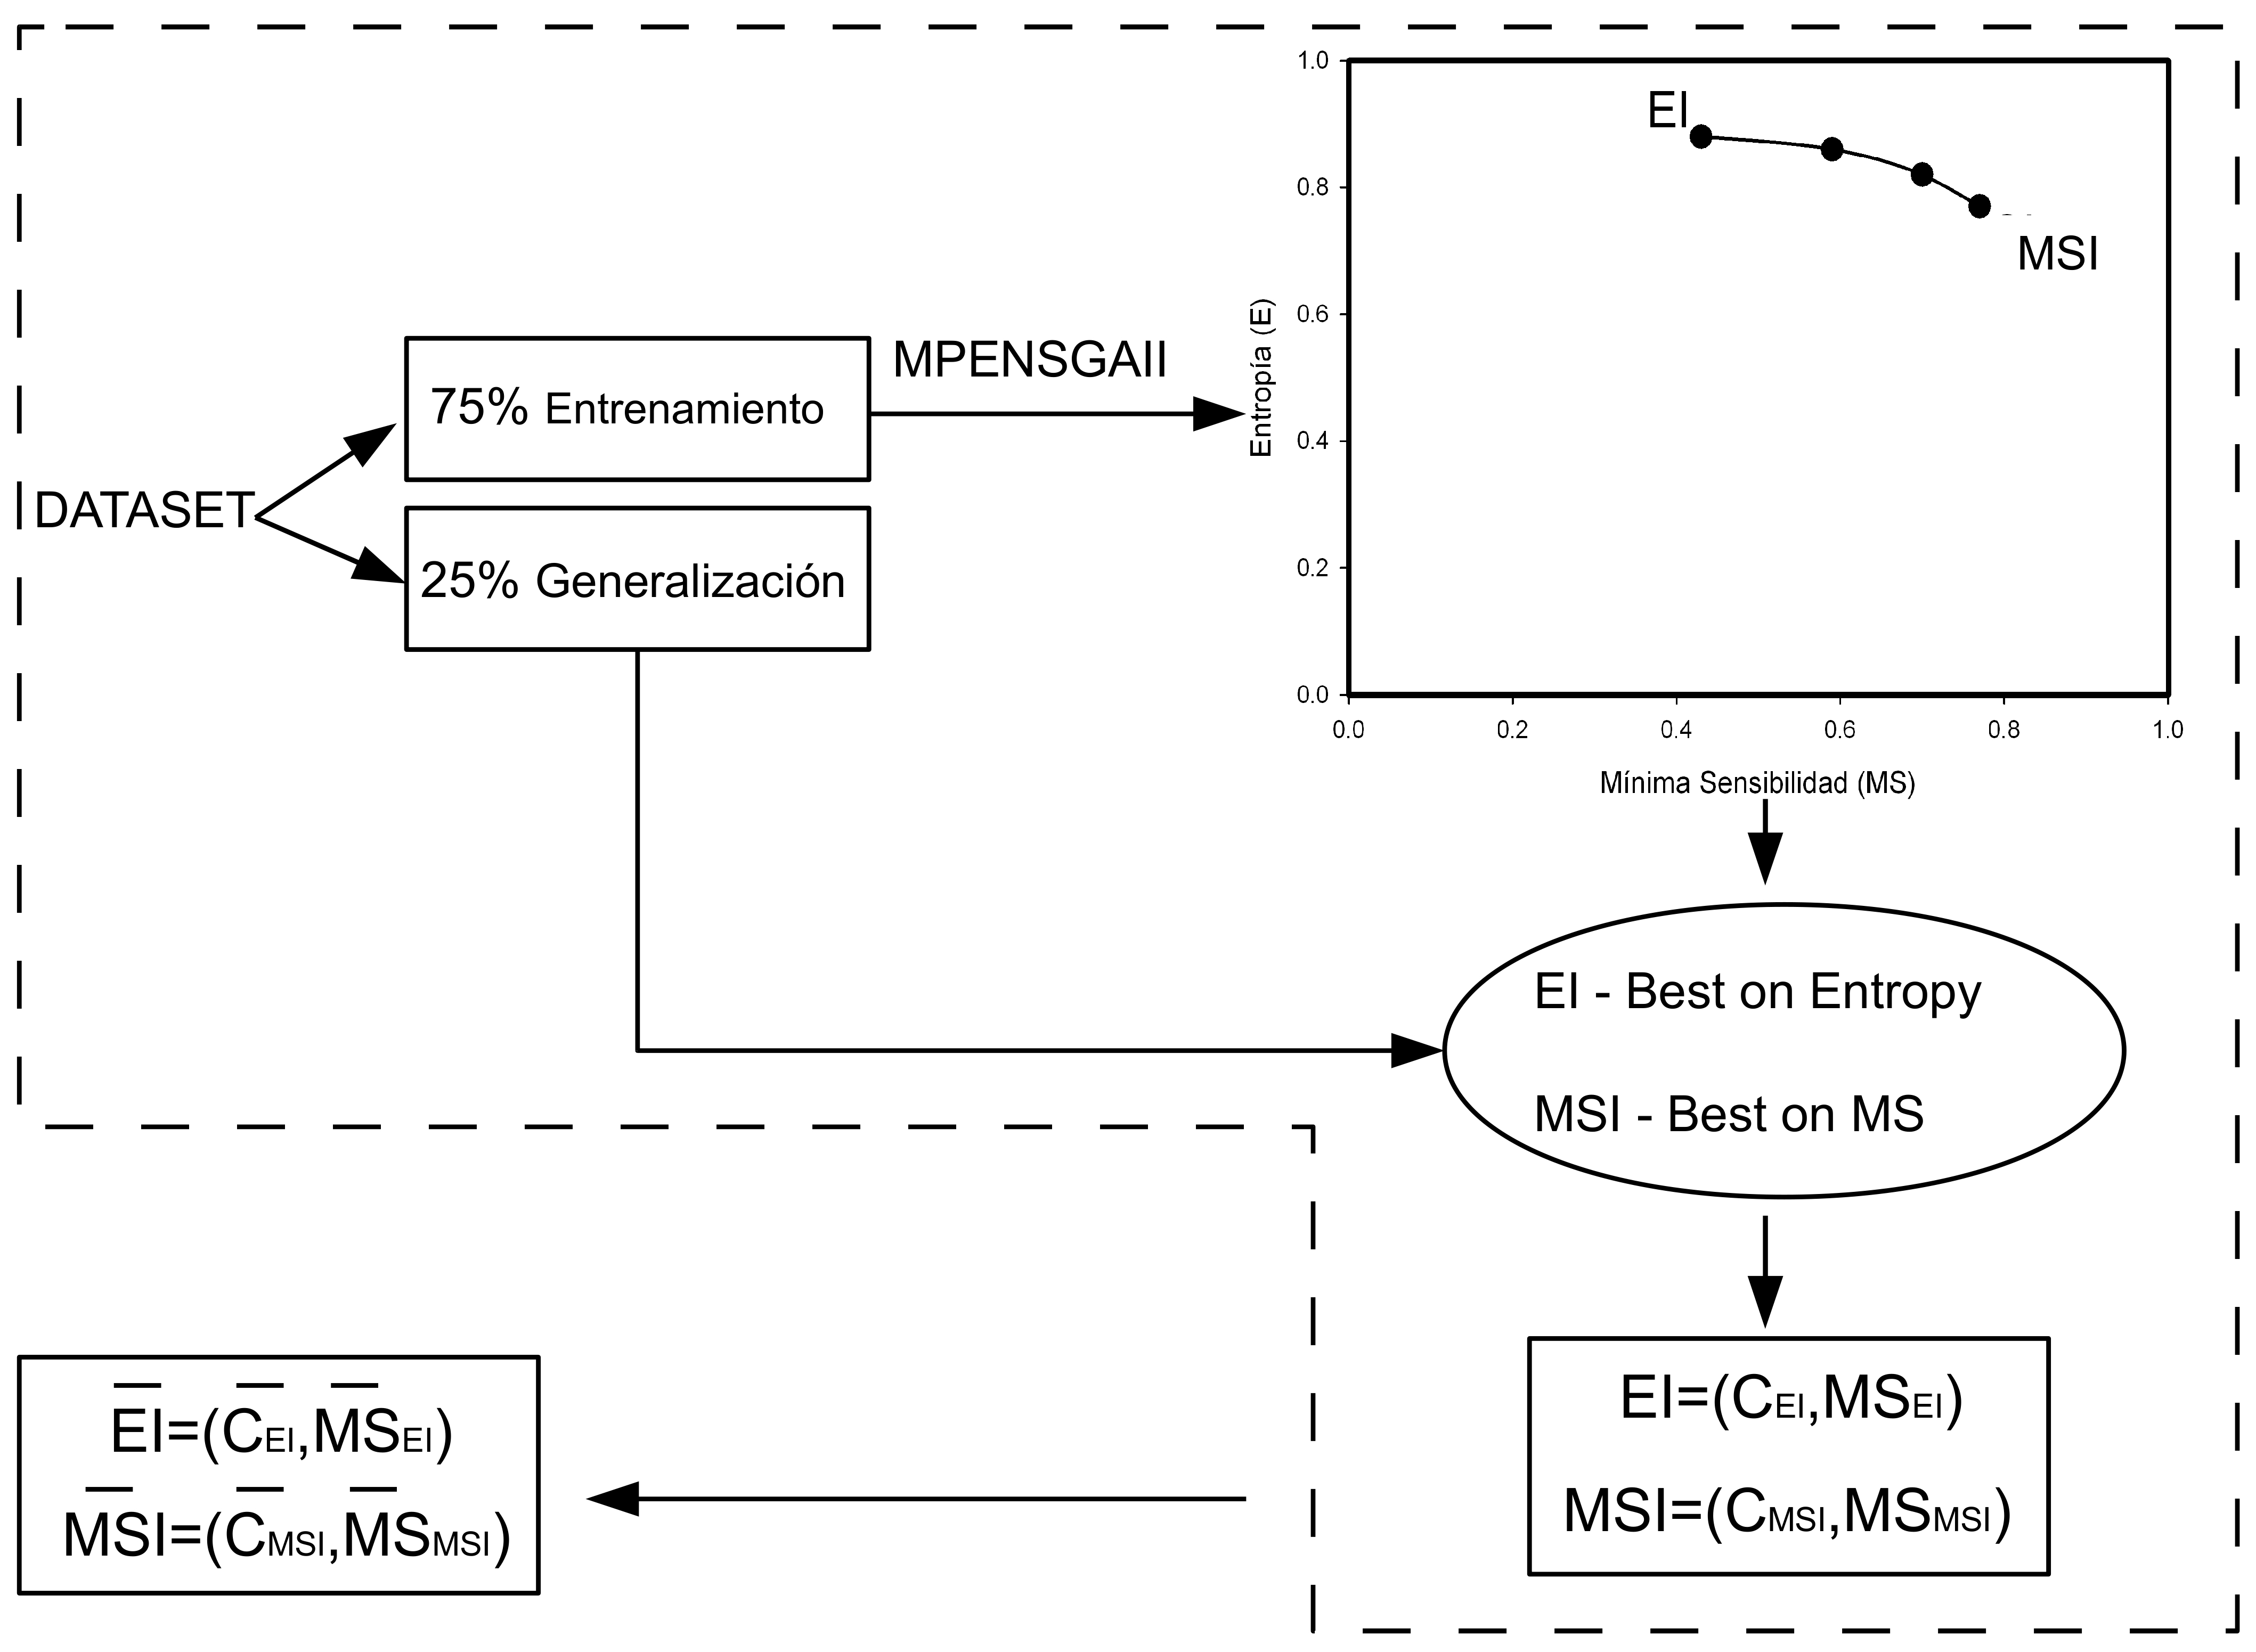
\includegraphics[keepaspectratio,width=13cm]{figuras/obtencionResultados.jpg}
\caption{Obtención de modelos a partir de MPENSGAII.}
\label{obtencionResultados}
\end{figure}

Una vez que tenemos los individuos del paso anterior se calcula su valor de precisión,
$C$, y de mínima sensibilidad, $MS$, sobre el conjunto de generalización. De esta manera,
tenemos para los extremos del frente dos pares de valores, $\displaystyle
EI=(C_{EI},MS_{EI})$ y
$\displaystyle MSI=(C_{MSI},MS_{MSI})$ de una ejecución de las 30 realizadas.

El proceso anterior se repite 30 veces obteniendo finalmente la media y la desviación
típica de los dos pares de valores para los individuos $EI$ y $MSI$, es decir,
$\displaystyle \overline{EI}=(\overline{C}_{EI},\overline{MS}_{EI})$ y
$\displaystyle \overline{MSI}=(\overline{C}_{MSI},\overline{MS}_{MSI})$, de forma que la
primera expresión muestra el rendimiento medio obtenido teniendo en cuenta solo los
mejores individuos en $E$, mientras que la segunda expresión muestra el rendimiento
medio teniendo en cuenta solo los mejores individuos en $MS$. Al
procedimiento de obtención automática del rendimiento medio teniendo en cuenta los
mejores individuos en $E$ (parte superior del frente) lo hemos llamado MPENSGAIIE, y al
procedimiento de obtención automática del rendimiento medio teniendo en cuenta los mejores
individuos en $MS$ (parte inferior del frente) lo hemos llamado MPENSGAIIS.

Todos los parámetros de MPENSGAII son comunes a los 18 experimentos, excepto $m$,
$M_{I}$, $M_{E}$ y el número de generaciones usadas, que al igual que para el
algoritmo  CBFEP depende del conjunto de datos. El valor de la población se ha
establecido en $N_{p}=100$. La probabilidad de mutación para cada operador es igual a
$1/5$. Para la mutación paramétrica hemos establecido valores de $r=0.95$ y de
temperatura inicial $T_{0}=1$. Para iRprop+, los parámetros adoptados son $\eta^{-}=0.5$
(tamaño de paso para el factor de decremento), $\eta^{+}=1.2$ (tamaño de paso para el
factor de incremento), $\bigtriangleup_{0} =0.0125$ (valor inicial de tamaño de paso para
los pesos, $\bigtriangleup_{ij}$),  $\bigtriangleup_{min} =0$ (tamaño mínimo de paso para
los pesos), $\bigtriangleup_{max} =50$ (tamaño máximo de paso para los pesos), $Epochs=25$
(número de épocas para la optimización local).

\subsection{Resultados} \label{resultadosMPENSGAII}
\noindent Hemos comparado MPENSGAII con dos algoritmos muy utilizados en el
entrenamiento de ANNs:
\begin{description}
\item[MPANN:] MPANN (\textit{Memetic Pareto Artificial Neural Networks})
\cite{Abbass2003} es un MOEA basado en DE \cite{Price2005} para el diseño de ANNs, que
optimiza dos objetivos: minimizar el $MSE$ y minimizar la complejidad de la red, teniendo
en cuenta el número de neuronas en capa oculta. MPANN utiliza el algoritmo BP como
procedimiento de LS.

Nosotros hemos implementado una versión de MPANN en Java utilizando el pseudocódigo
descrito en \cite{Abbass2003}, ya que no hay una versión de este algoritmo de libre
disposición. Para el algoritmo de LS hemos utilizado iRprop+ en vez de BP,
mejorando el procedimiento con respecto a BP \cite{Igel2000}. También hemos añadido a
la implementación la obtención de la $MS$ de todas las clases. MPANN utiliza la misma
estrategia automática de obtención de resultados
utilizada con MPENSGAII, es decir, se seleccionan los extremos del frente de Pareto
teniendo en cuenta a los mejores individuos en $MSE$ y a los mejores individuos en complejidad
(neuronas ocultas). Así, a las dos metodologías automáticas de obtención de resultados se
le ha llamado MPANN-MSE y MPANN-HN.

\item[TRAINDIFFEVOL:] TRAINDIFFEVOL (\textit{Differential Evolution Training Algorithm for
Feed-Forward Neural Networks}) \cite{Jarno2003} es un algoritmo mono-objetivo para
entrenar perceptrones multicapa mediante el error cuadrático medio de los
pesos regularizado (\textit{Mean Square Error Regularized}, MSEREG) y está basado en DE
\cite{Price2005}.

Para poder realizar adecuadamente una comparación con los resultados obtenidos con este
método hemos modificado el código fuente de TRAINDIFFEVOL, de forma que se pueda obtener
la sensibilidad para cada una de las clases de un problema y así poder calcular
$MS$. TRAINDIFFEVOL está disponible en la web en código Matlab
\footnote{http://www.it.lut.fi/project/nngenetic}.
\end{description}

Las tablas \ref{tabla2MPENSGAII} y \ref{tabla2MPENSGAII-b} presentan los valores de las medias y
desviaciones típicas
para $C$ y $MS$ en generalización para los mejores modelos en cada ejecución y para cada
conjunto de datos.

\begin{landscape}
\tabcolsep 2.5pt
\scriptsize
\begin{longtable}{cccccccc}
\caption{Resultados estadísticos para MPENSGAIIE, MPENSGAIIS, TRAINDIFFEVOL, MPANN-MSE y
MPANN-HN en generalización para los conjuntos de datos binarios.}
\label{tabla2MPENSGAII} \\
\hline
\rowcolor[rgb]{0.70,0.85,1}\textbf{Conjunto} & \textbf{Algoritmo} & $\mathbf{C(\%)}$ &
$\mathbf{MS(\%)}$ & \textbf{Conjunto} & \textbf{Algoritmo} & $\mathbf{C(\%)}$ &
$\mathbf{MS(\%)}$ \\ \hline
\multicolumn{8}{>{\columncolor[rgb]{0.70,0.85,1}}c}{\textbf{Dos clases}} \\ \hline
\endfirsthead
\hline
% \rowcolor[rgb]{0.70,0.85,1}\textbf{Conjunto} & \textbf{Algoritmo} & $\mathbf{C(\%)}$ &
% $\mathbf{MS(\%)}$ & \textbf{Conjunto} & \textbf{Algoritmo} & $\mathbf{C(\%)}$ &
% $\mathbf{MS(\%)}$ \\
% \hline \multicolumn{8}{r}{{Continúa en la siguiente página}} \\ \hline
% \endfoot
% \hline \hline
% \endlastfoot
\rowcolor[rgb]{0.86,0.94,1}Australian Card & MPENSGA2E & \textit{88.07$\pm$1.57} &
\textit{86.13$\pm$2.73} & Breast Cancer & MPENSGA2E & \textbf{69.34$\pm$2.30} &
\textit{28.89$\pm$9.10} \\
\rowcolor[rgb]{0.86,0.94,1}& MPENSGA2S & \textbf{88.25$\pm$1.39} & \textbf{86.84$\pm$2.00}
&  & MPENSGA2S & 63.99$\pm$3.11 & \textbf{53.09$\pm$6.58} \\
\rowcolor[rgb]{0.86,0.94,1}& TRAINDIFFEVOL & 81.93$\pm$7.78 & 72.90$\pm$18.04\textbf{} &
& TRAINDIFFEVOL & \textit{68.94$\pm$2.82} & 26.35$\pm$11.17 \\
\rowcolor[rgb]{0.86,0.94,1}& MPANN-MSE & 87.59$\pm$1.18\textbf{} & 85.95$\pm$1.98\textbf{}
&  & MPANN-MSE & 66.53$\pm$3.07 & 28.73$\pm$14.23\textbf{} \\
\rowcolor[rgb]{0.86,0.94,1}& MPANN-HN & 87.78$\pm$2.49\textbf{} & 85.83$\pm$4.43\textbf{}
&  & MPANN-HN & 66.53$\pm$3.07 & 28.41$\pm$14.34\textbf{} \\ \hline
\rowcolor[rgb]{0.86,0.94,1}Breast Cancer Wisconsin & MPENSGA2E & 95.87$\pm$0.61 &
90.94$\pm$1.68 & German & MPENSGA2E & \textbf{75.31$\pm$1.44} & \textit{51.16$\pm$4.10} \\
\rowcolor[rgb]{0.86,0.94,1}& MPENSGA2S & 95.60$\pm$0.85 & 90.72$\pm$1.84\textbf{} &  &
MPENSGA2S & 71.55$\pm$1.87 & \textbf{68.80$\pm$3.11} \\
\rowcolor[rgb]{0.86,0.94,1}& TRAINDIFFEVOL & 93.98$\pm$1.75 & 86.22$\pm$4.69\textbf{} &  &
TRAINDIFFEVOL & 71.73$\pm$2.11 & 28.36$\pm$19.90 \\
\rowcolor[rgb]{0.86,0.94,1}& MPANN-MSE & \textit{96.04$\pm$1.08} & \textit{92.75$\pm$3.40}
&  & MPANNMSE & 73.61$\pm$1.80 & 48.89$\pm$5.33\textbf{} \\
\rowcolor[rgb]{0.86,0.94,1}& MPANN-HN & \textbf{96.27$\pm$1.00} & \textbf{93.30$\pm$3.36}
&  & MPANN-HN & \textit{73.76$\pm$1.77} & 48.76$\pm$5.44\textbf{} \\ \hline
\rowcolor[rgb]{0.86,0.94,1}Heart Statlog & MPENSGA2E & \textbf{78.28$\pm$1.76} &
61.89$\pm$2.09 & Ionosphere & MPENSGA2E & \textbf{92.65$\pm$2.22} &
\textbf{82.71$\pm$5.36} \\
\rowcolor[rgb]{0.86,0.94,1}& MPENSGA2S & \textit{77.50$\pm$1.73} & \textit{62.67$\pm$2.38}
&  & MPENSGA2S & \textit{92.08$\pm$2.30} & \textit{82.40$\pm$4.14} \\
\rowcolor[rgb]{0.86,0.94,1}& TRAINDIFFEVOL & 76.32$\pm$2.02 & 60.00$\pm$3.82 &  &
TRAINDIFFEVOL & 85.23$\pm$4.68 & 65.31$\pm$9.11 \\
\rowcolor[rgb]{0.86,0.94,1}& MPANN-MSE & 76.91$\pm$1.10 & \textbf{62.68$\pm$2.21} &  &
MPANN-MSE & 91.10$\pm$2.37 & 79.17$\pm$5.99 \\
\rowcolor[rgb]{0.86,0.94,1}& MPANN-HN & 76.91$\pm$1.10 & \textbf{62.68$\pm$2.21} &  &
MPANN-HN & 91.10$\pm$2.37 & 79.17$\pm$5.99 \\ \hline
\rowcolor[rgb]{0.86,0.94,1}Pima & MPENSGA2E & \textbf{78.99$\pm$1.81} &
\textit{60.45$\pm$2.59} & Vote & MPENSGA2E & \textbf{94.74$\pm$0.87} &
\textbf{93.42$\pm$1.70} \\
\rowcolor[rgb]{0.86,0.94,1}& MPENSGA2S & 76.96$\pm$2.09\textbf{} & \textbf{72.69$\pm$3.07}
&  & MPENSGA2S & \textit{94.68$\pm$0.91} & \textit{93.38$\pm$1.61}\textbf{\textit{}} \\
\rowcolor[rgb]{0.86,0.94,1}& TRAINDIFFEVOL & 70.59$\pm$3.50 & 37.29$\pm$19.74 &  &
TRAINDIFFEVOL & 93.39$\pm$1.69 & 91.99$\pm$1.69 \\
\rowcolor[rgb]{0.86,0.94,1}& MPANN-MSE & \textit{78.54$\pm$1.80} & 59.65$\pm$3.71 &  &
MPANN-MSE & 94.19$\pm$1.28 & 92.53$\pm$2.34 \\
\rowcolor[rgb]{0.86,0.94,1}& MPANN-HN & 78.28$\pm$2.03 & 58.86$\pm$3.86 &  & MPANN-HN &
94.19$\pm$1.28 & 92.53$\pm$2.34 \\ \hline
\multicolumn{8}{l}{Los mejores resultados están en \textbf{negrita} y los segundos mejores
resultados se encuentran en \textit{itálica}.} \\
\end{longtable}
\end{landscape}

\begin{landscape}
\tabcolsep 2.5pt
\scriptsize
\begin{longtable}{cccccccc}
\caption{Resultados estadísticos para MPENSGAIIE, MPENSGAIIS, TRAINDIFFEVOL, MPANN-MSE y
MPANN-HN en generalización para los conjuntos de datos multiclase.}
\label{tabla2MPENSGAII-b} \\
\hline
\rowcolor[rgb]{0.70,0.85,1}\textbf{Conjunto} & \textbf{Algoritmo} & $\mathbf{C(\%)}$ &
$\mathbf{MS(\%)}$ & \textbf{Conjunto} & \textbf{Algoritmo} & $\mathbf{C(\%)}$ &
$\mathbf{MS(\%)}$ \\ \hline
\multicolumn{8}{>{\columncolor[rgb]{0.70,0.85,1}}c}{\textbf{Multi-clase}} \\ \hline
\endfirsthead
\hline
% \rowcolor[rgb]{0.70,0.85,1}\textbf{Conjunto} & \textbf{Algoritmo} & $\mathbf{C(\%)}$ &
% $\mathbf{MS(\%)}$ & \textbf{Conjunto} & \textbf{Algoritmo} & $\mathbf{C(\%)}$ &
% $\mathbf{MS(\%)}$ \\
% \hline
% \multicolumn{8}{>{\columncolor[rgb]{0.70,0.85,1}}c}{\textbf{Multi-clase}} \\ \hline
% \endhead
% \multicolumn{8}{>{\columncolor[rgb]{0.70,0.85,1}}c}{\textbf{Multi-clase}} \\ \hline
\rowcolor[rgb]{0.86,0.94,1}Autos & MPENSGA2E & \textbf{66.67$\pm$4.06} &
\textit{39.64$\pm$14.91} & Balance & MPENSGA2E & \textbf{94.02$\pm$1.53} & 42.66$\pm$17.00
\\
\rowcolor[rgb]{0.86,0.94,1}& MPENSGA2S & \textit{66.04$\pm$4.78} &
\textbf{42.28$\pm$10.97} &  & MPENSGA2S & 92.48$\pm$2.16 & \textbf{83.74$\pm$8.19} \\
\rowcolor[rgb]{0.86,0.94,1}& TRAINDIFFEVOL & 26.79$\pm$7.49 & 0.00$\pm$0.00 &  &
TRAINDIFFEVOL & 87.12$\pm$2.56 & 2.00$\pm$6.10 \\
\rowcolor[rgb]{0.86,0.94,1}& MPANN-MSE & 48.42$\pm$3.71 & 0.00$\pm$0.00 &  & MPANN-MSE &
\textit{92.94$\pm$1.81} & \textit{60.00$\pm$14.14} \\
\rowcolor[rgb]{0.86,0.94,1} & MPANN-HN & 48.42$\pm$3.71 & 0.00$\pm$0.00 &  & MPANN-HN &
\textit{92.94$\pm$1.81} & \textit{60.00$\pm$14.14} \\ \hline
\rowcolor[rgb]{0.86,0.94,1}BTX & MPENSGA2E & \textbf{85.56$\pm$5.66} &
\textbf{61.11$\pm$12.63} & Gene & MPENSGA2E & \textit{86.42$\pm$2.04} &
\textit{80.85$\pm$3.45}\textbf{\textit{}} \\
\rowcolor[rgb]{0.86,0.94,1} & MPENSGA2S & \textit{85.40$\pm$5.99} &
\textit{60.00$\pm$13.56} &  & MPENSGA2S & \textbf{86.47$\pm$2.28} &
\textbf{81.77$\pm$2.77} \\
\rowcolor[rgb]{0.86,0.94,1} & TRAINDIFFEVOL & 71.11$\pm$3.94 & 1.11$\pm$6.09 &  &
TRAINDIFFEVOL & 60.88$\pm$7.12 & 34.97$\pm$9.11 \\
\rowcolor[rgb]{0.86,0.94,1} & MPANN-MSE & 72.38$\pm$10.85 & 13.33$\pm$29.81 &  & MPANN-MSE
& 75.11$\pm$4.98 & 36.20$\pm$3.87 \\
\rowcolor[rgb]{0.86,0.94,1} & MPANN-HN & 69.52$\pm$11.46 & 13.33$\pm$29.81 &  & MPANN-HN &
75.11$\pm$4.98 & 36.20$\pm$3.87  \\ \hline
\rowcolor[rgb]{0.86,0.94,1}Iris & MPENSGA2E & \textbf{97.18$\pm$0.78} &
\textbf{91.54$\pm$2.35} & Lymphography & MPENSGA2E & \textbf{85.05$\pm$4.24} &
\textbf{5.17$\pm$19.67} \\
\rowcolor[rgb]{0.86,0.94,1} & MPENSGA2S & 96.50$\pm$1.43\textbf{} & 89.74$\pm$3.69 &  &
MPENSGA2S & \textbf{85.05$\pm$4.24} & \textbf{5.17$\pm$19.67} \\
\rowcolor[rgb]{0.86,0.94,1}& TRAINDIFFEVOL & \textit{97.18$\pm$1.03} &
\textit{91.54$\pm$3.10} &  & TRAINDIFFEVOL & \textit{81.98$\pm$4.62} & 0.00$\pm$0.00 \\
\rowcolor[rgb]{0.86,0.94,1}& MPANN-MSE & 95.29$\pm$9.85 & 86.15$\pm$29.51 &  & MPANN-MSE
& 80.45$\pm$5.96 & 0.00$\pm$0.00 \\
\rowcolor[rgb]{0.86,0.94,1} & MPANN-HN & 94.52$\pm$11.24 & 83.84$\pm$33.70 &  & MPANN-HN &
80.72$\pm$6.05 & 0.00$\pm$0.00 \\ \hline
\rowcolor[rgb]{0.86,0.94,1}Newthyroid & MPENSGA2E &
\textit{95.12$\pm$2.31}\textbf{\textit{}} & \textit{74.81$\pm$10.08} & Post-op & MPENSGA2E
& 67.83$\pm$3.89 & 0.00$\pm$0.00\textbf{} \\
\rowcolor[rgb]{0.86,0.94,1} & MPENSGA2S & \textbf{95.56$\pm$2.15} &
\textbf{75.08$\pm$10.67} &  & MPENSGA2S & 38.12$\pm$16.6 & \textbf{3.96$\pm$12.97} \\
\rowcolor[rgb]{0.86,0.94,1}& TRAINDIFFEVOL & 91.11$\pm$4.77 & 59.47$\pm$22.74 &  &
TRAINDIFFEVOL & \textbf{69.57$\pm$1.14} & 0.00$\pm$0.00 \\
\rowcolor[rgb]{0.86,0.94,1} & MPANN-MSE & 94.87$\pm$3.81 & 72.11$\pm$22.29 &  & MPANN-MSE
& \textit{68.84$\pm$2.81} & 0.00$\pm$0.00 \\
\rowcolor[rgb]{0.86,0.94,1} & MPANN-HN & 94.87$\pm$3.81 & 72.11$\pm$22.29 &  & MPANN-HN &
\textit{68.84$\pm$2.81} & 0.00$\pm$0.00 \\ \hline
\rowcolor[rgb]{0.86,0.94,1}Vowel & MPENSGA2E & \textbf{79.51$\pm$3.19} &
\textit{57.39$\pm$9.84} & Yeast & MPENSGA2E & \textbf{59.91$\pm$0.98} & 0.00$\pm$0.00 \\
\rowcolor[rgb]{0.86,0.94,1} & MPENSGA2S & \textit{77.36$\pm$3.90} &
\textbf{57.97$\pm$6.07} &  & MPENSGA2S & \textit{53.21$\pm$4.49} &
\textbf{12.13$\pm$12.20} \\
\rowcolor[rgb]{0.86,0.94,1} & TRAINDIFFEVOL & 40.83$\pm$2.80 & 0.00$\pm$0.00 &  &
TRAINDIFFEVOL & 37.61$\pm$5.16 & 0.00$\pm$0.00 \\
\rowcolor[rgb]{0.86,0.94,1} & MPANN-MSE & 41.66$\pm$4.21 & 0.00$\pm$0.00 &  & MPANN-MSE &
48.87$\pm$3.53 & 0.00$\pm$0.00 \\
\rowcolor[rgb]{0.86,0.94,1} & MPANN-HN & 41.66$\pm$4.21 & 0.00$\pm$0.00 &  & MPANN-HN &
48.87$\pm$3.53 & 0.00$\pm$0.00 \\ \hline
\multicolumn{8}{l}{Los mejores resultados están en \textbf{negrita} y los segundos mejores
resultados se encuentran en \textit{itálica}.} \\
\end{longtable}
\end{landscape}

En general, los mejores resultados se obtienen con MPENSGAIIE o MPENSGAIIS en todos los
conjuntos de datos, excepto para Breast Cancer Wisconsin, Heart-Statlog y Post-op. La tabla
\ref{tabla3MPENSGAII} resume los resultados, incluyendo la precisión
media en generalización, $\overline{C}_{G}(\%)$, y la $MS$ media,
$\overline{MS}_{G}(\%)$, para todos los conjuntos y métodos. Se muestra además el
orden de cada método en cada conjunto ($R=1$ para el método con mejor
rendimiento y $R=5$ para el peor), y el orden medio en $C$
($\overline{R}_{CG}$) y en $MS$ ($\overline{R}_{MSG}$). Si se
analizan estos resultados podemos realizar los siguientes comentarios:
\begin{enumerate}
	\item La metodología MPENSGAIIE obtiene el mejor resultado en $C$ en 13 de los 18
conjuntos, el segundo mejor resultado en otros tres, la mejor media en precisión
($\overline{C}_{G}=82.81\%$) y el mejor orden medio ($\overline{R}_{CG}$). En
$MS$, la metodología MPENSGAIIE obtiene el mejor resultado en 5 conjuntos y el segundo
mejor
resultado en otros 8. También obtiene el segundo mejor resultado medio en $MS$
($\overline{MS}_{G}=55.70\%$) y el segundo mejor orden medio en $MS$
($\overline{R}_{MSG}$). Teniendo en cuesta estos resultados, deberíamos utilizar esta
metodología (desde un punto de vista cuantitativo) si nuestro objetivo es obtener
clasificadores con buenos resultados en $C$ y resultados más que aceptables en $MS$.
\begin{table}[!htb]
\renewcommand{\arraystretch}{1.2}
\caption{Media en precisión ($\overline{C}_G(\%)$) y mínima sensibilidad
($\overline{MS}_G(\%)$) en generalización, orden medio en precisión
($\overline{R}_{CG}$) y orden medio en mínima sensibilidad
($\overline{R}_{MSG}$) en generalización para los diferentes métodos evaluados con los 18
conjuntos.}
\label{tabla3MPENSGAII}
\centering
\begin{tabular}{ccccc} \hline
\rowcolor[rgb]{0.70,0.85,1} &
\multicolumn{2}{>{\columncolor[rgb]{0.70,0.85,1}}c}{\textbf{Precisión}} &
\multicolumn{2}{>{\columncolor[rgb]{0.70,0.85,1}}c}{\textbf{Mínima Sensibilidad}} \\
\cline{2-5}
\rowcolor[rgb]{0.70,0.85,1}\textbf{Algoritmo} & $\mathbf{\overline{C}_{G}(\%)}$ &
$\mathbf{\overline{R}_{CG}}$ & \textbf{$\mathbf{\overline{MS}_{G}(\%)}$} &
$\mathbf{\overline{R}_{MSG}}$ \\ \hline
\rowcolor[rgb]{0.86,0.94,1}MPENSGA2E & \textbf{82.81} & \textbf{1.56} & \textit{55.70} &
\textit{2.17} \\
\rowcolor[rgb]{0.86,0.94,1}MPENSGA2S & \textit{79.82} & \textit{2.75} & \textbf{62.32} &
\textbf{1.56} \\
\rowcolor[rgb]{0.86,0.94,1}TRAINDIFFEVOL & 73.26 & 3.97 & 37.10 & 4.21 \\
\rowcolor[rgb]{0.86,0.94,1}MPANNMSE & 76.85 & 3.36 & 44.44 & 3.41 \\
\rowcolor[rgb]{0.86,0.94,1}MPANN-HN & 76.68 & 3.36 & 44.26 & 3.65 \\ \hline
\multicolumn{5}{l}{El mejor resultado se encuentra en \textbf{negrita} y el segundo mejor}\\
\multicolumn{5}{l}{resultado en \textit{itálica}.} \\
\end{tabular}
\end{table}
	\item Por otro lado, los resultados de MPENSGA2S muestran que, en $C$, es el mejor
	método para 4 conjuntos de datos, y el segundo mejor para otros 7, obteniendo el segundo mejor
resultado medio en precisión ($\overline{C}_{G}=79.82\%$) y el segundo mejor
orden medio en precisión ($\overline{R}_{CG}=2.75$). En $MS$, obtiene los
mejores resultados para 12 conjuntos de datos, el segundo mejor resultado para otros 4, la mejor
$MS$ media ($\overline{MS}_{G}=62.32\%$) y el mejor orden medio en
$MS$ ($\overline{R}_{MSG}=1.56$). Esta metodología se debería escoger si
nuestro objetivo es obtener clasificadores con buenos resultados en $MS$ y con valores
más que aceptables en $C$.
	\item Hemos observado una tendencia a clasificar la clase mayoritaria al analizar las
matrices de confusión mediante los modelos optimizados con el algoritmo TRAINDIFFEVOL.
Por esta razón TRAINDIFFEVOL obtiene mejores resultados cuando se aplica a problemas de
clasificación binaria o problemas bien balanceados, pero obtiene un peor rendimiento
cuando se aplica a problemas multi-clase o problemas muy desbalanceados.
	\item MPENSGA2E obtiene el mejor valor en $C$ y en $MS$ para
los conjuntos Ionosphere, Vote, BTX, Iris y Lymphography.
	\item MPENSGA2S obtiene el mejor valor valor en $C$ y $MS$ para Australian Card, Gene,
Lymphography y Newthyroid.
	\item Los conjuntos Autos, Lymphography, Post-op y Yeast necesitan de una mención
especial, ya que son problemas de difícil clasificación para todas las metodologías,
dado que están desbalanceados (observe en la tabla \ref{tabla2MPENSGAII} como estos
conjuntos tienen un valor de $p^*$ menor a $0.05$), haciendo que una mejora en
$MS$ sea difícil. A pesar de que el porcentaje de clasificación es aceptable, el valor de
$MS$ es muy bajo, debido a que la clase minoritaria tiene 3, 2, 2 y 5 patrones
respectivamente en cada uno de los conjuntos de datos mencionados. MPENSGA2S obtiene en $MS$: un
$42.28\%$ en media en Autos, un $5.17\%$
en Lymphography, un $3.96\%$ en Post-op y un $12.13\%$ en Yeast, sin reducir
dramáticamente la media en $C$ (ver tabla \ref{tabla2MPENSGAII}), mientras que el valor
de $MS$ con otras metodologías tienen una media de $0.00\%$. Cuando el problema está
muy desbalanceado, como en el caso de Autos y Lymphography, es muy difícil mejorar los
niveles de $MS$. Estos casos sugieren que en un futuro trabajo se integren técnicas de
remuestreo \cite{Chawla2002} en nuestra metodología.
\end{enumerate}

Para determinar si hay diferencias estadísticas significativas en los resultados
observados para cada método con los diferentes conjuntos de datos, se han realizado dos
test de Friedman no paramétricos \cite{Friedman1940} con el orden de $C_{G}$ y
$MS_{G}$ de los mejores modelos. El uso de test no paramétricos está justificado en este
caso, ya que un test previo de normalidad de Kolmogorov-Smirnof y de igualdad de
varianzas de Levene de los valores de $C_{G}$ y $MS_{G}$, hace que se
rechace esta hipótesis. Hay que observar los altos valores
de varianza obtenidos en la evaluación de $MS$ y las diferencias existentes entre las
varianzas en todos los métodos. Los test muestran que el efecto del método usado para
clasificación es estadísticamente significativo para valores de $C_{G}$ en un nivel de
significación del 5\%, ya que el intervalo de confianza es $C_{0}=(0,F_{0.05}=2.51)$ y
el valor de la distribución estadística $F$ es $F^*=8.58\notin C_{0}$. Para valores de
$MS_{G}$, los test también muestran la significación del método aplicado, ya que el
intervalo de confianza es $C_{0}=(0,F_{0.05}=2.52)$ y el valor de la distribución
estadística $F$ es $F^*=14.75\notin C_{0}$. Por tanto, rechazamos la hipótesis nula que
indica que todos los algoritmos son iguales en rendimiento con respecto a los
ordenes medios de $C$ y $MS$.

En base a los rechazos de hipótesis comentados, se aplican dos test no paramétricos de
Bonferroni-Dunn \cite{Dunn1961,Hochberg1987}, uno para los valores de $C_{G}$ y otro para
los de $MS_{G}$. El objetivo de estos test es valorar si el mejor algoritmo en
rendimiento para cada una de las medidas evaluadas (MPENSGAIIE para $C_{G}$ y MPENSGAIIS
para $MS_{G}$) obtiene diferencias significativas en el orden medio cuando se
compara con otros métodos. Así, MPENSGAIIE es el método de control cuando se comparan
los valores de los ordenes medios en $C_{G}$ y MPENSGAIIS cuando se comparan
los valores de los ordenes medios en $MS_{G}$. Los resultados del test
Bonferroni-Dunn para $\alpha=0.1$ y $\alpha=0.05$ se muestran en la tabla
\ref{tabla4MPENSGAII}, usando los correspondientes valores críticos para el test
bilateral de Bonferroni-Dunn.

\begin{table}[!htb]
\renewcommand{\arraystretch}{1.2}
\caption{Orden medio, valores de diferencia crítica y diferencias
de orden de los test de Bonferroni-Dunn aplicados para la precisión y la
mínima sensibilidad, usando MPENSGAIIE y MPENSGAIIS como métodos de control.}
\label{tabla4MPENSGAII}
\centering
\small
\tabcolsep 1pt
\begin{tabular}{cccc} \hline
\multicolumn{2}{>{\columncolor[rgb]{0.70,0.85,1}}c}{\textbf{Precisión}} &
\multicolumn{2}{>{\columncolor[rgb]{0.70,0.85,1}}c}{\textbf{Mínima sensibilidad}}\\ \hline
\multicolumn{2}{>{\columncolor[rgb]{0.70,0.85,1}}c}{\textbf{Método de control}} &
\multicolumn{2}{>{\columncolor[rgb]{0.70,0.85,1}}c}{\textbf{Método de control}} \\ \hline
\rowcolor[rgb]{0.70,0.85,1}$\mathbf{\bar{R}}$ & \textbf{MPENSGAIIE} & $\mathbf{\bar{R}}$ &
\textbf{MPENSGAIIS} \\ \hline
\rowcolor[rgb]{0.86,0.94,1}$\bar{R}_{(1)}=1.56$ & $-$ & $\bar{R}_{(1)}=2.17$ &
$\left|\bar{R}_{(2)}-\bar{R}_{(1)}\right|=0.62$ \\
\rowcolor[rgb]{0.86,0.94,1}$\bar{R}_{(2)}=2.75$ &
$\left|\bar{R}_{(1)}-\bar{R}_{(2)}\right|={\rm1}.{\rm 19}_{\circ }^{+}$ &
$\bar{R}_{(2)}=1.56$ & $-$ \\
\rowcolor[rgb]{0.86,0.94,1}$\bar{R}_{(3)}=3.97$ &
$\left|\bar{R}_{(1)}-\bar{R}_{(3)}\right|={\rm 2}.{\rm 42}_{\bullet }^{+} $ &
$\bar{R}_{(3)}=4.21$ & $\left|\bar{R}_{(2)}-\bar{R}_{(3)} \right|={\rm 2}.{\rm
65}_{\bullet }^{+} $ \\
\rowcolor[rgb]{0.86,0.94,1}$\bar{R}_{(4)}=3.36$ &
$\left|\bar{R}_{(1)}-\bar{R}_{(4)}\right|=1.81_{\bullet }^{+} $ &
$\bar{R}_{(4)}=3.41$ & $\left|\bar{R}_{(2)}-\bar{R}_{(4)}
\right|={\rm 1}.{\rm 85}_{\bullet }^{+} $ \\
\rowcolor[rgb]{0.86,0.94,1}$\bar{R}_{(5)}=3.36$ & $\left|\bar{R}_{(5)}-\bar{R}_{(3)}
\right|=1.81_{\bullet }^{+} $ & $\bar{R}_{(5)} =3.65$ &
$\left|\bar{R}_{(2)} -\bar{R}_{(5)} \right|={\rm 2}.0{\rm
9}_{\bullet }^{+} $ \\ \hline
\multicolumn{2}{>{\columncolor[rgb]{0.86,0.94,1}}c}{$DC_{(\alpha=0.1)}=1.18;DC_{
	(\alpha=0.05)}=1.32$} &
\multicolumn{2}{>{\columncolor[rgb]{0.86,0.94,1}}c}{$DC_{(\alpha =0.1)}=1.22\text{;}
DC_{(\alpha =0.05)}=1.32$} \\\hline
\multicolumn{4}{l}{$\bullet$ Diferencias estadísticas significativas con $\alpha=0.05$.}\\
\multicolumn{4}{l}{$\circ$ Diferencias estadísticas significativas con $\alpha=0.1$.}\\
\multicolumn{4}{l}{$+$ Diferencia a favor del método de control.}\\
\multicolumn{4}{l}{(1):MPENSGAIIE; (2):MPENSGAIIS; (3):TRAINDIFFEVOL; (4):MPANN-MSE;}\\
\multicolumn{4}{l}{(5):MPANN-HN; DC:Diferencia crítica.}
\end{tabular}
\end{table}

A partir de los resultados de estos test, podemos concluir que existen diferencias
significativas en el rango medio de los valores de $C_{G}$ para $\alpha=0.05$ cuando se
compara MPENSGAIIE con las otras metodologías, a excepción de la comparación con
MPENSGAIIS, donde existen diferencias pero para $\alpha=0.1$.

Con respecto al método MPENSGAIIS, podemos concluir que existen diferencias
significativas en el rango medio de los valores de $MS_{G}$ para $\alpha=0.05$ cuando se
compara MPENSGAIIS con las otras metodologías, a excepción de la comparación con
MPENSGAIIE, donde existen diferencias pero para $\alpha=0.1$.

Es importante destacar que ambas metodologías, MPENSGAIIE y \\ MPENSGAIIS, obtienen un
buen
equilibrio entre los dos objetivos ($C$ y $MS$) y esto hace que sea difícil obtener
diferencias significativas entre los dos métodos. Esto se puede observar
especialmente en aquellos conjuntos de datos donde los individuos que se obtienen están
cerca de los valores óptimos en $C$ y $MS$.

Por tanto, podemos concluir que las metodologías utilizadas, MPENSGAIIE y MPENSGAIIS, para
la obtención de modelos basados en el concepto de dominancia y óptimo de Pareto, resultan
adecuadas para mejorar
uno de los objetivos, sin causar un empeoramiento excesivo en el otro. Los resultados
obtenidos están en consonancia con los frentes de Pareto de $MS$ frente a $E$
($A_{1}$ frente a $A_{2}$) en entrenamiento, así como los
gráficos de $MS$ y $C$, $(A_{1},C)$ en generalización, que se
muestran en las figuras \ref{tanda1} a la \ref{tanda6}. En estas figuras podemos ver los resultados
obtenidos para cada conjunto en el plano $(MS,C)$ (ver sección \ref{propiedades} del capítulo
\ref{medidasRendimiento}). Los gráficos están divididos en gráficos de entrenamiento
$(A_{1},A_{2})$, y en gráficos de generalización $(A_{1},C)$.

El procedimiento para los gráficos mencionados es el siguiente:
En cada una de las 30 ejecuciones llevadas a cabo con cada algoritmo y con cada
conjunto de datos, se obtienen sus 30 respectivos frentes de Pareto. A partir de aquí, se
selecciona el primer frente de Pareto de los 30 obtenidos, concretamente el frente que
presenta el mejor individuo en $E$ en entrenamiento en la última generación del
proceso evolutivo. En los gráficos de entrenamiento se muestran los frentes obtenidos
(primer frente y restantes) siendo $A_{1}$ y $A_{2}$ los objetivos que guían el algoritmo.
Los gráficos de generalización muestran los valores de $MS$ y $C$ de los modelos MLP que
se obtuvieron en entrenamiento, y a los que se les aplica el conjunto de
generalización,
mostrando la bondad de clasificación y su proximidad al punto $(1,1)$ en el plano
$(MS,C)$. Es importante observar que los puntos (clasificadores) que se encuentran en el
plano $(MS,C)$ ya no forman frente de Pareto (se les ha aplicado el conjunto de
generalización), y que los individuos que formaban el primer frente de Pareto en
entrenamiento en el gráfico $(A_{1},A_{2})$, pueden estar situados dentro del plano
$(MS,C)$ en una región peor que otros individuos de frentes inferiores. Esto se debe a
que no existe una relación matemática exacta entre el entrenamiento en $E$ y la
generalización en $C$, puesto que los modelos obtenidos pueden presentar un
sobre-entrenamiento.

En los gráficos $(MS,C)$, en general, y para conjuntos lo suficientemente
balanceados, los objetivos suelen estar relacionados para valores bajos de $C$ y $MS$,
mientras que para niveles altos de $MS$ y $C$ son objetivos en conflicto (ver sección
\ref{ms-c} y \ref{propiedades} del capítulo\ref{medidasRendimiento}). Para
conjuntos muy desbalanceados, un incremento en $C$ no implica un incremento en
$MS$. Se puede observar como en algunos conjuntos como Breast Cancer, German y
Pima, el tamaño (cardinalidad) del frente de Pareto es relativamente grande comparada con
otros conjuntos como Autos, Lymphography y Vote, ya que existe relación entre el número de
puntos del frente de Pareto, el tamaño de cada clase del problema y el valor de $p^*$.

\clearpage
\begin{figure}[!htb]
\centering
	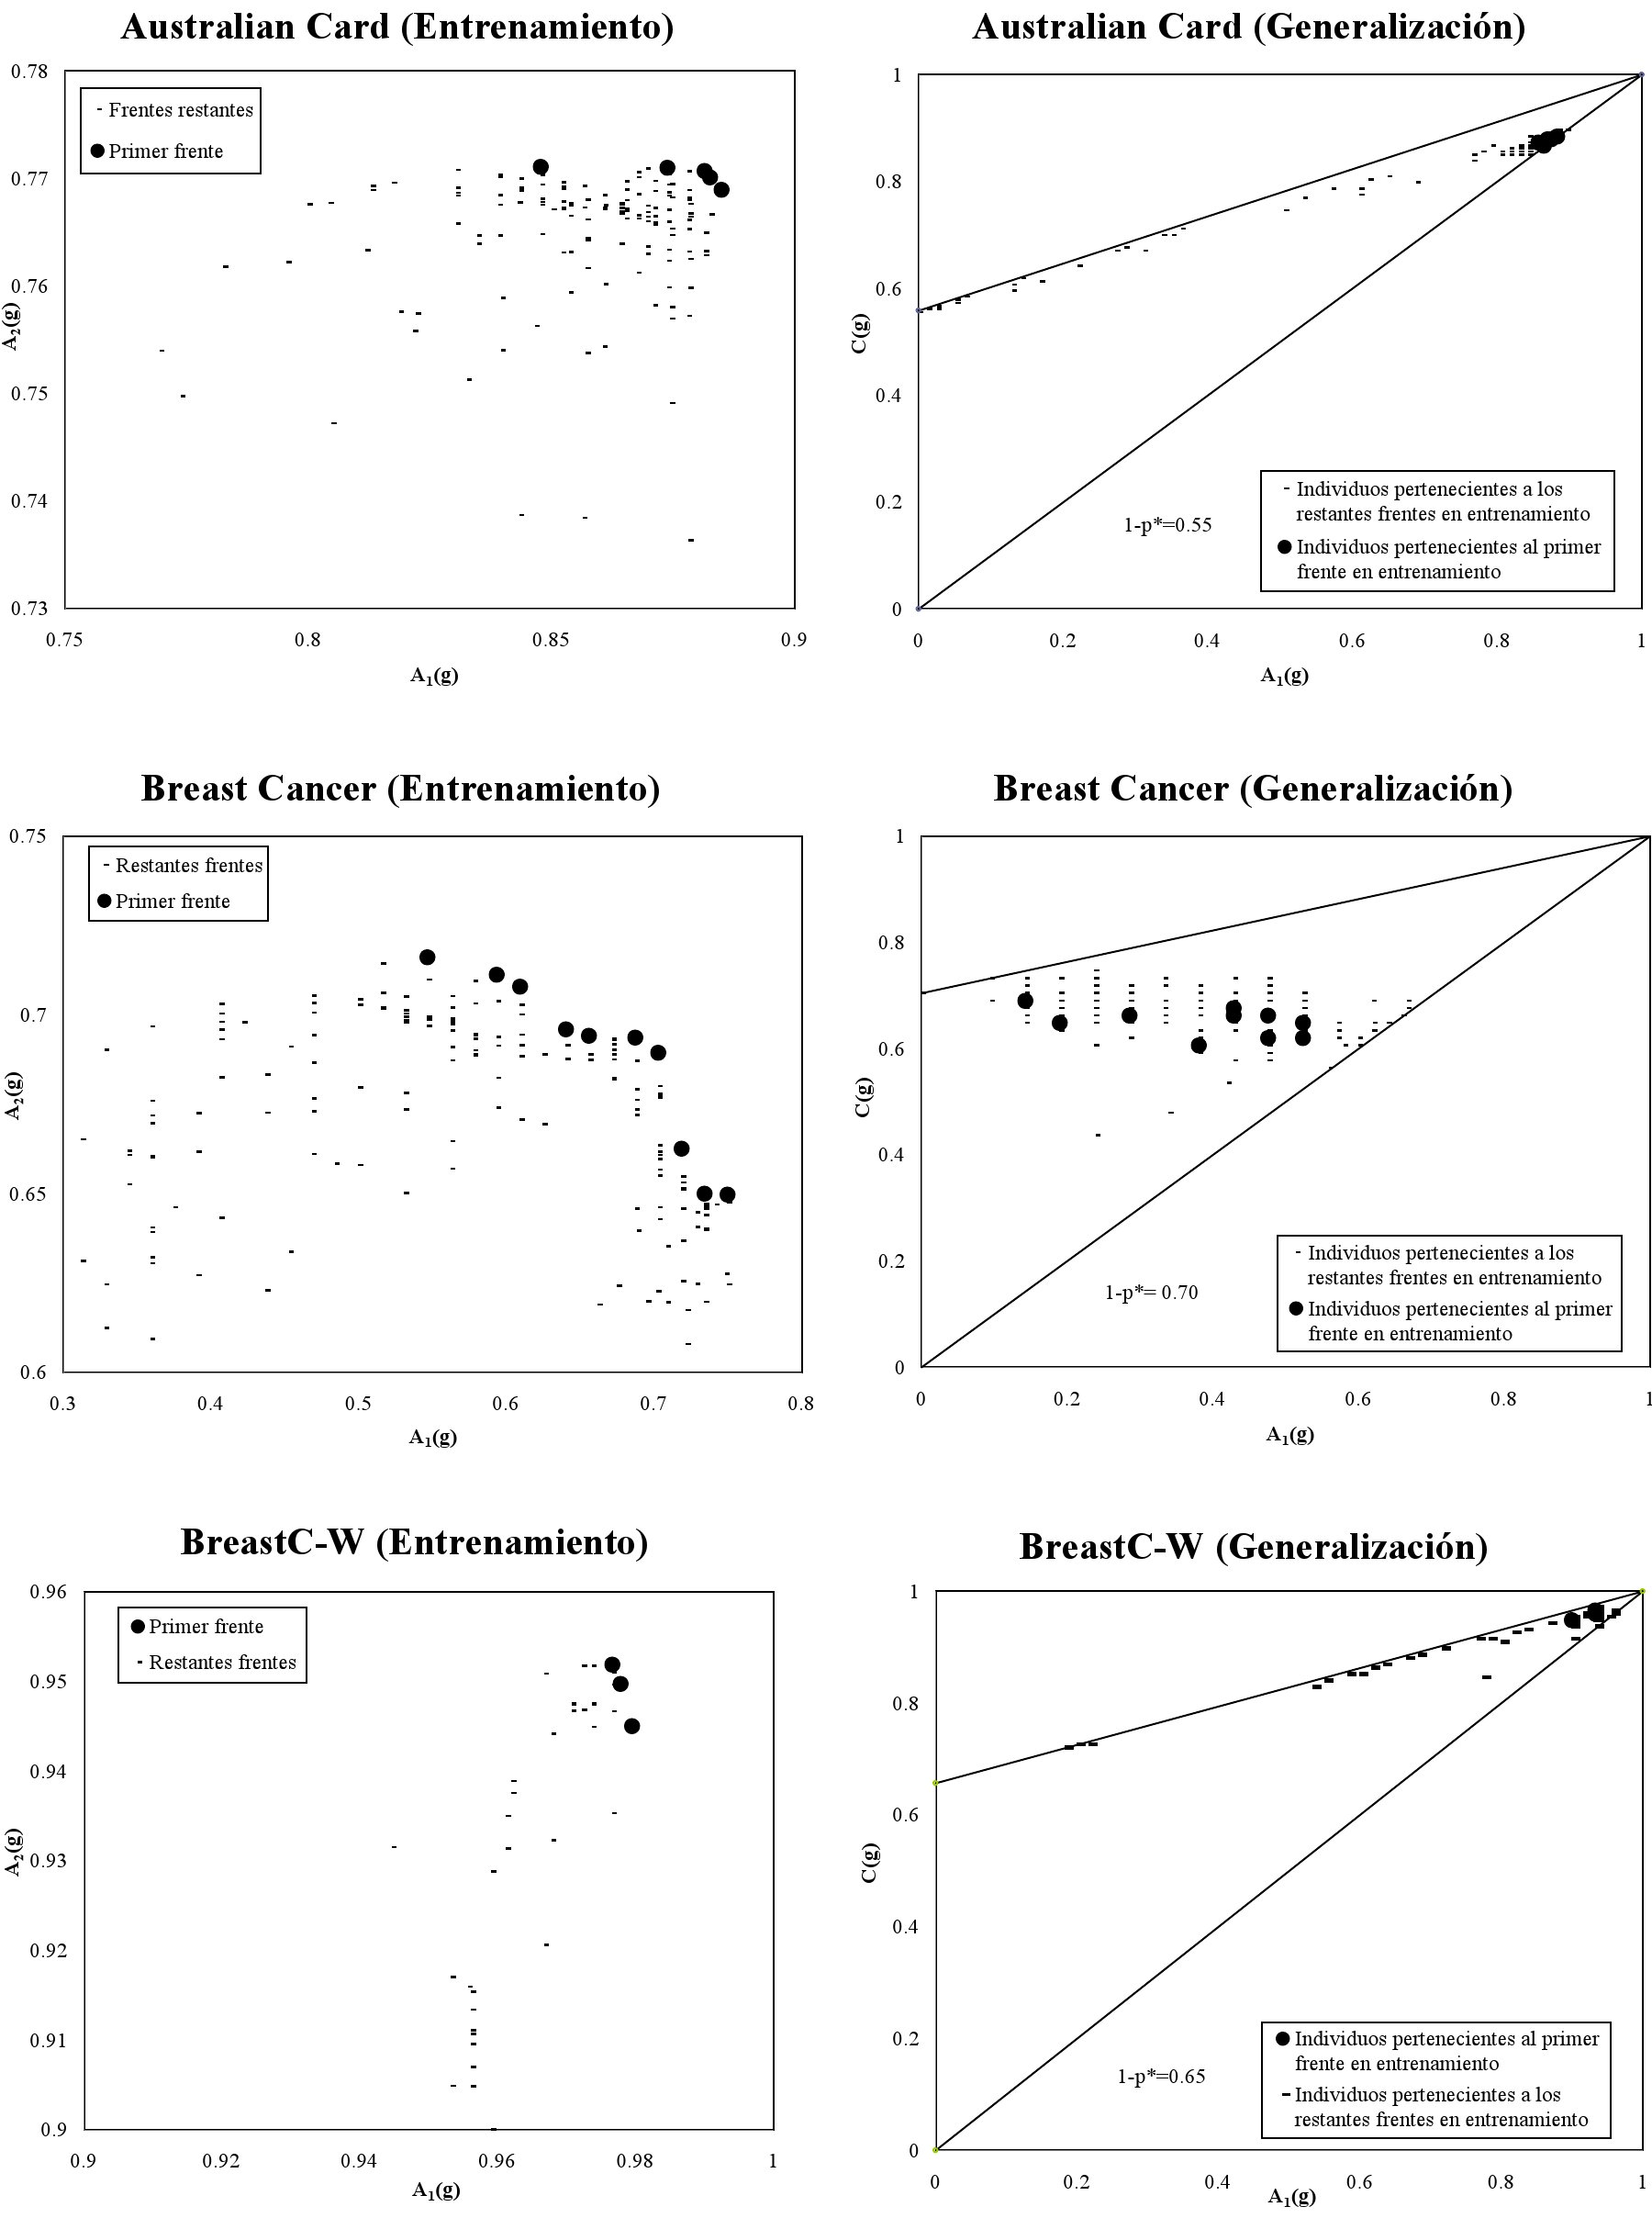
\includegraphics[keepaspectratio,width=13cm]{figuras/tanda1.jpg}
\caption{Frente de Pareto en entrenamiento $(A_{1},A_{2})$, y valores asociados a
$(A_{1},C)$ en generalización para los conjuntos Australian Card, Breast Cancer y
Breast Cancer Wisconsin.}
\label{tanda1}
\end{figure}

\begin{figure}[!htb]
\centering
	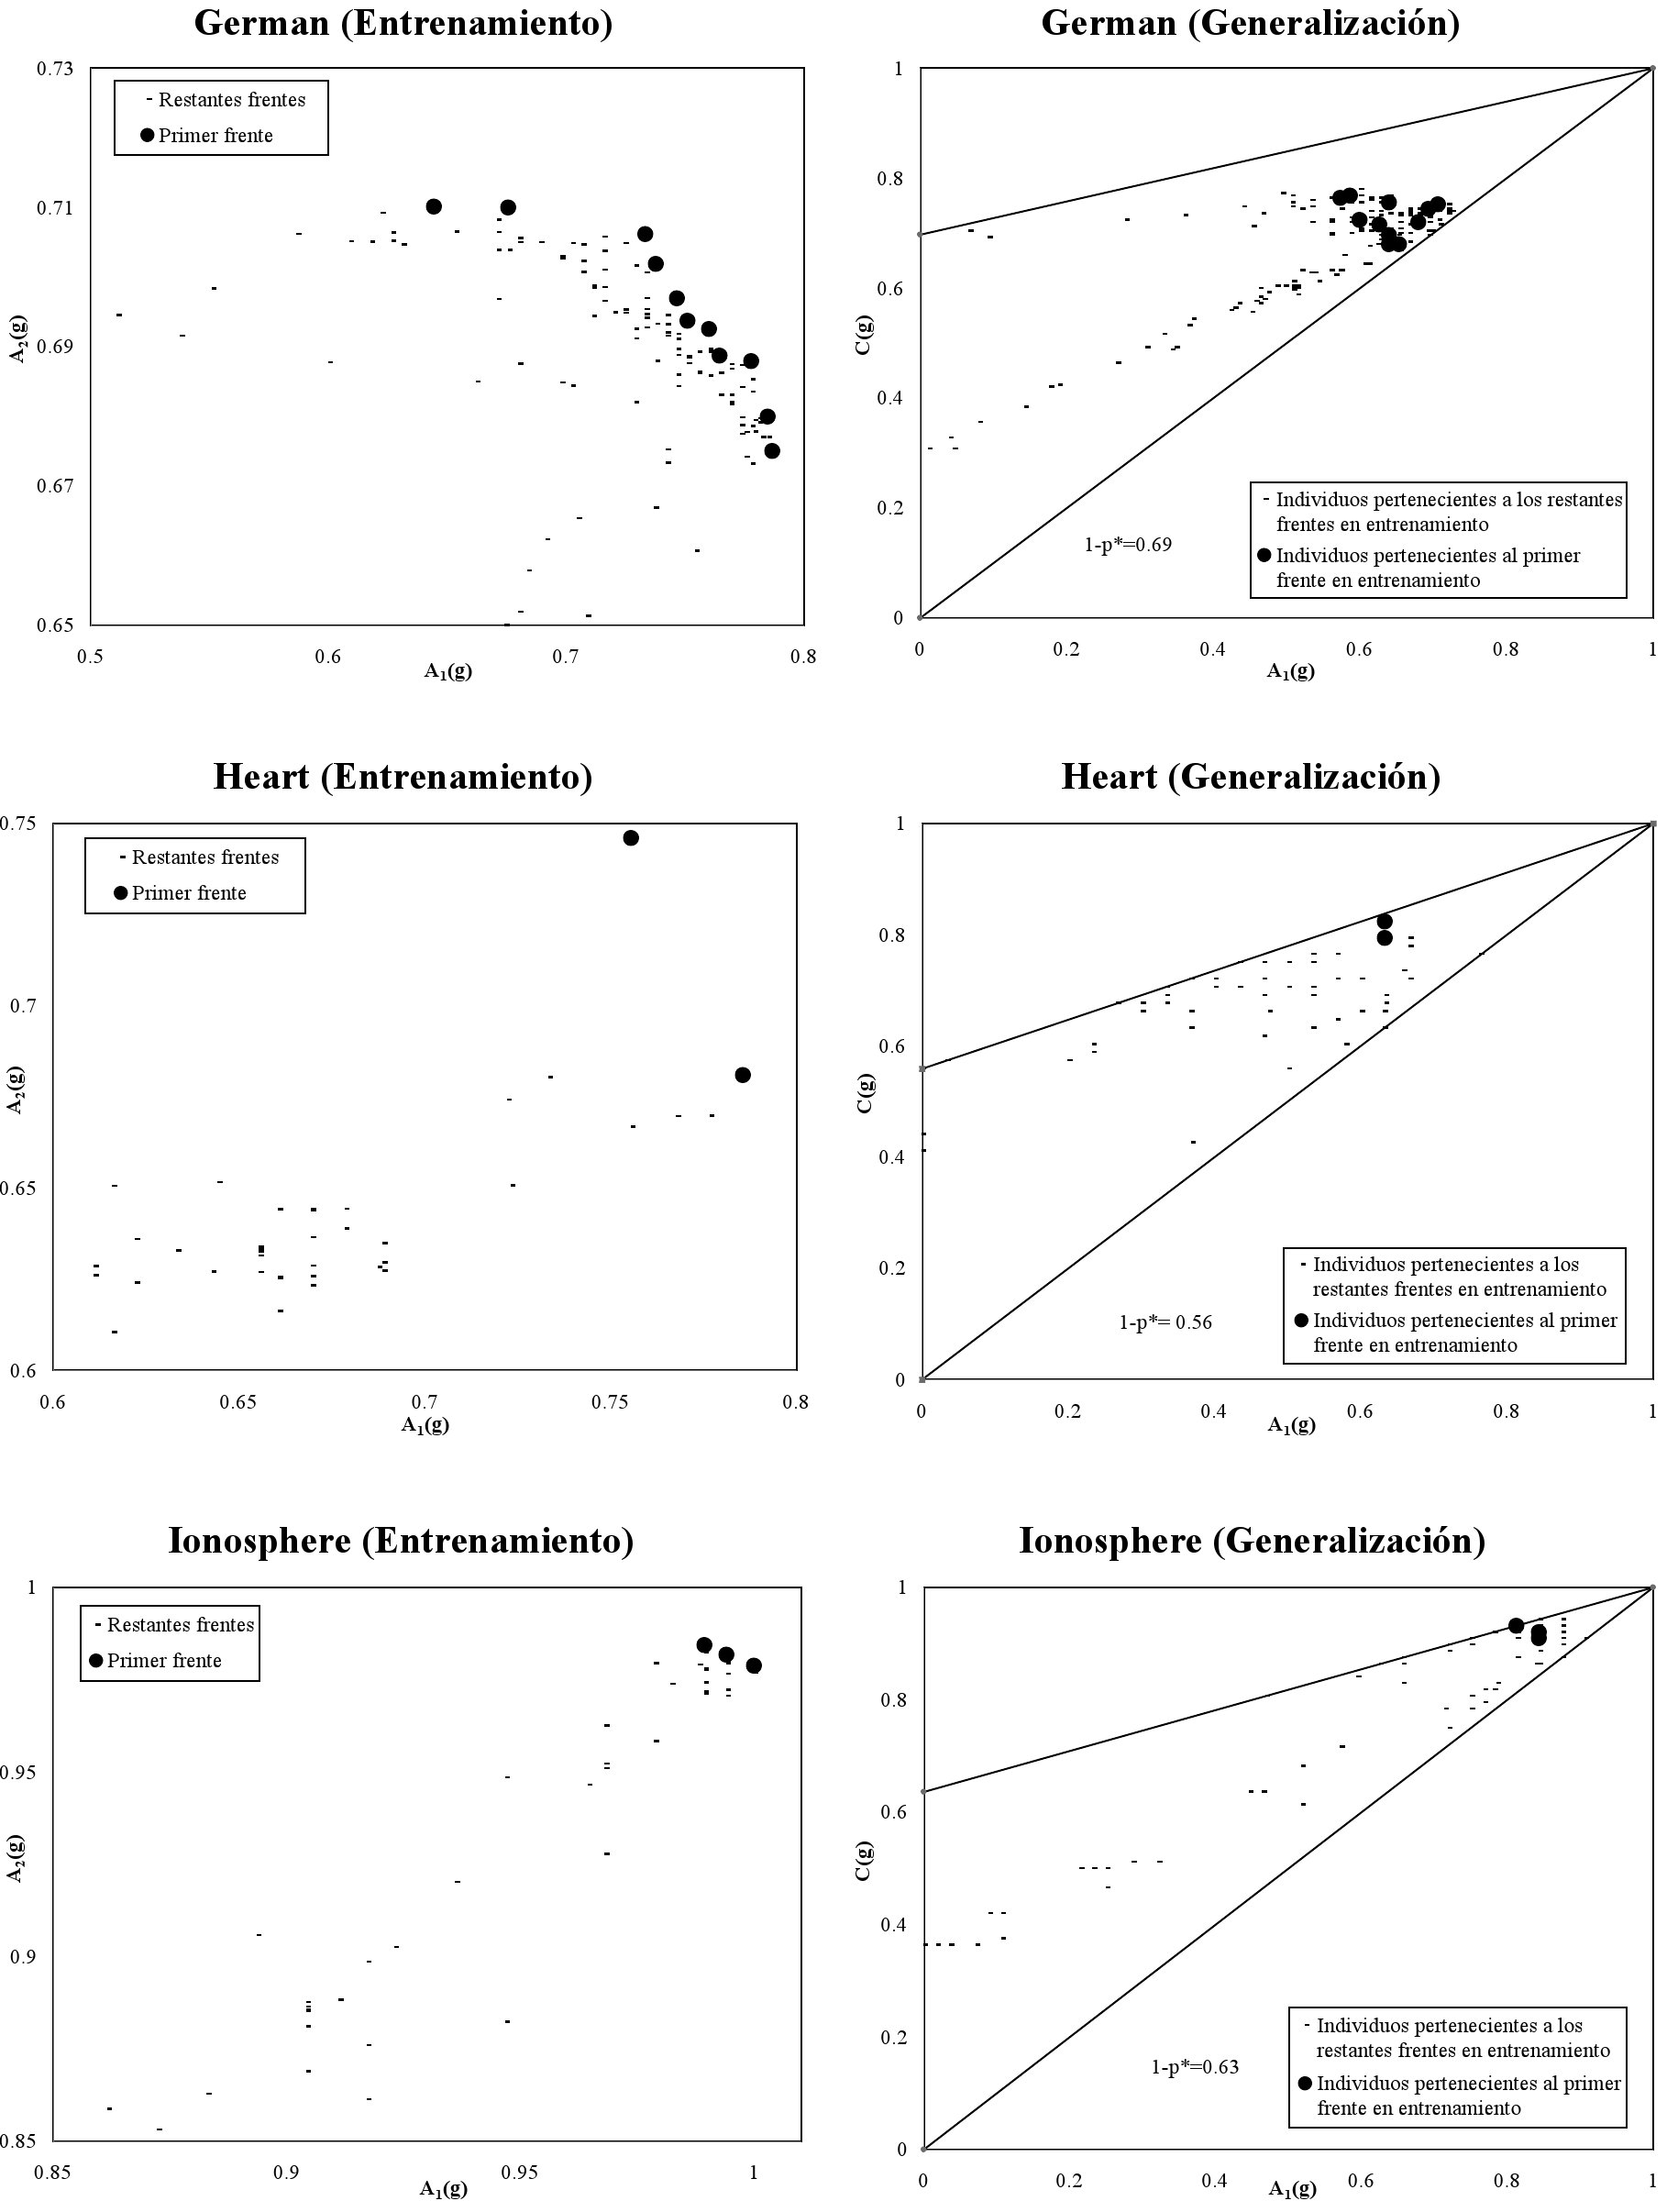
\includegraphics[keepaspectratio,width=13cm]{figuras/tanda2.jpg}
\caption{Frente de Pareto en entrenamiento $(A_{1},A_{2})$, y valores asociados a
$(A_{1},C)$ en generalización para los conjuntos German, Heart e Ionosphere.}
\label{tanda2}
\end{figure}

\begin{figure}[!htb]
\centering
	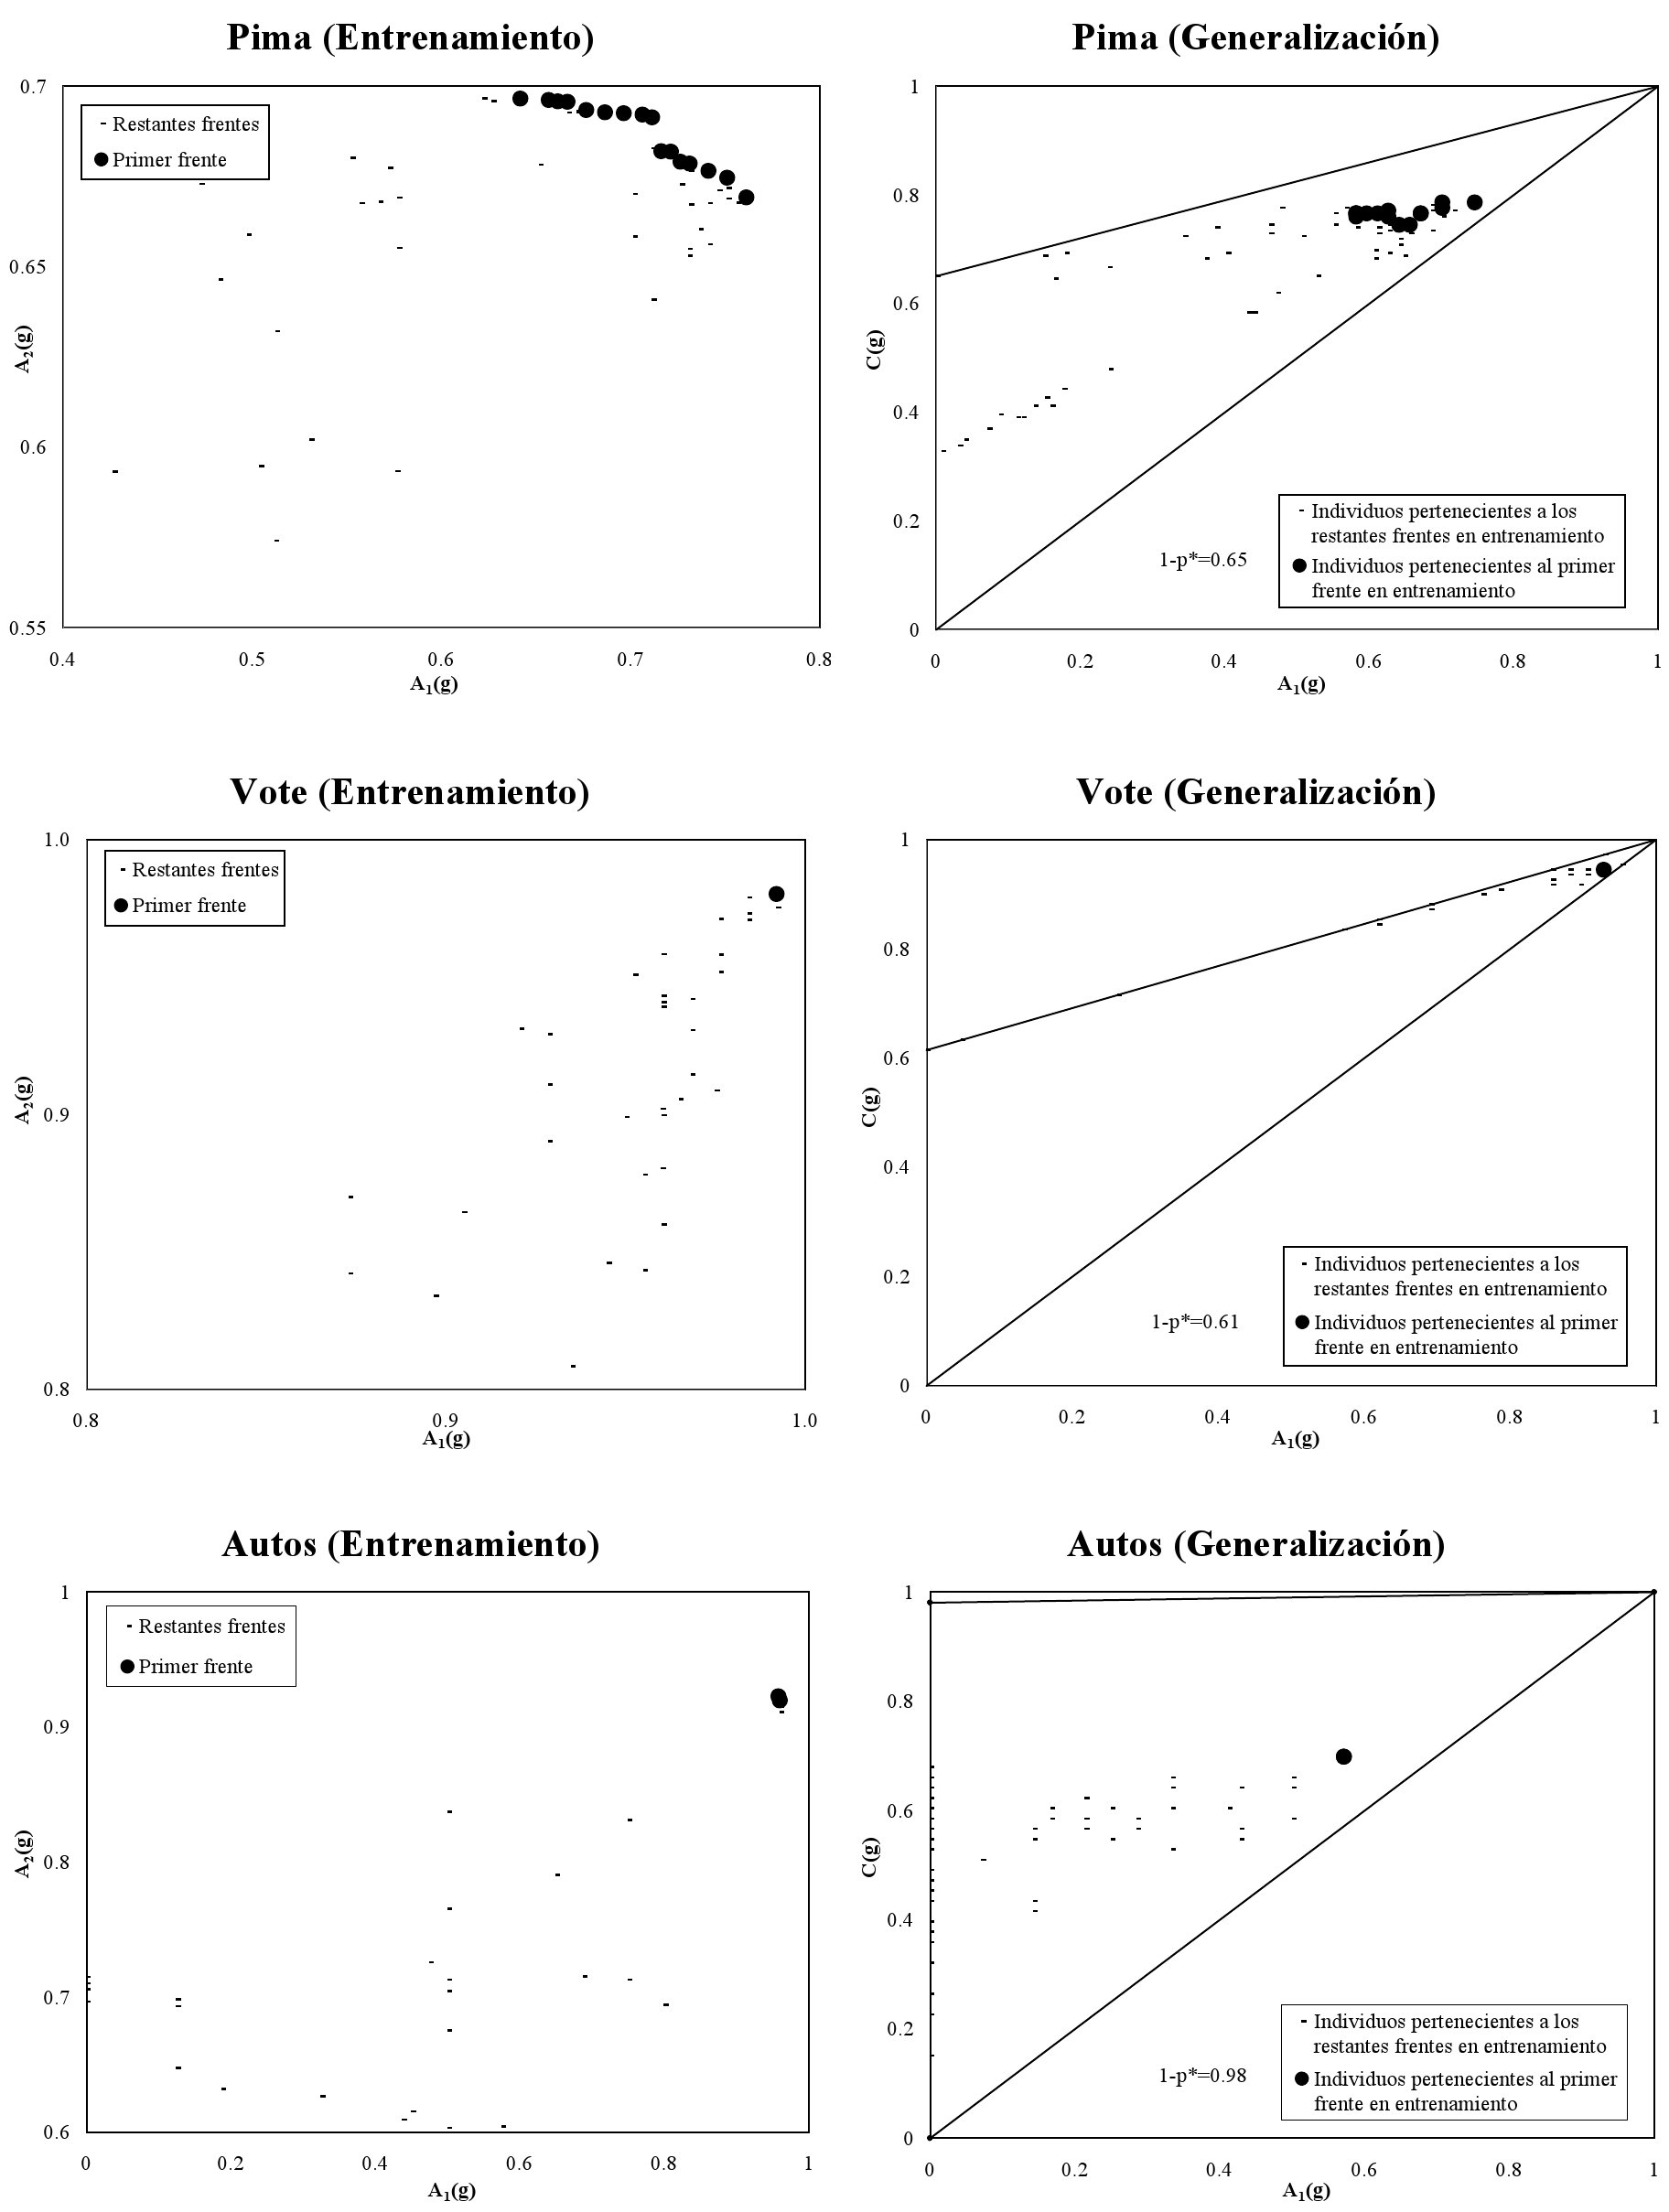
\includegraphics[keepaspectratio,width=13cm]{figuras/tanda3.jpg}
\caption{Frente de Pareto en entrenamiento $(A_{1},A_{2})$, y valores asociados a
$(A_{1},C)$ en generalización para los conjuntos Pima, Vote y Autos.}
\label{tanda3}
\end{figure}

\begin{figure}[!htb]
\centering
	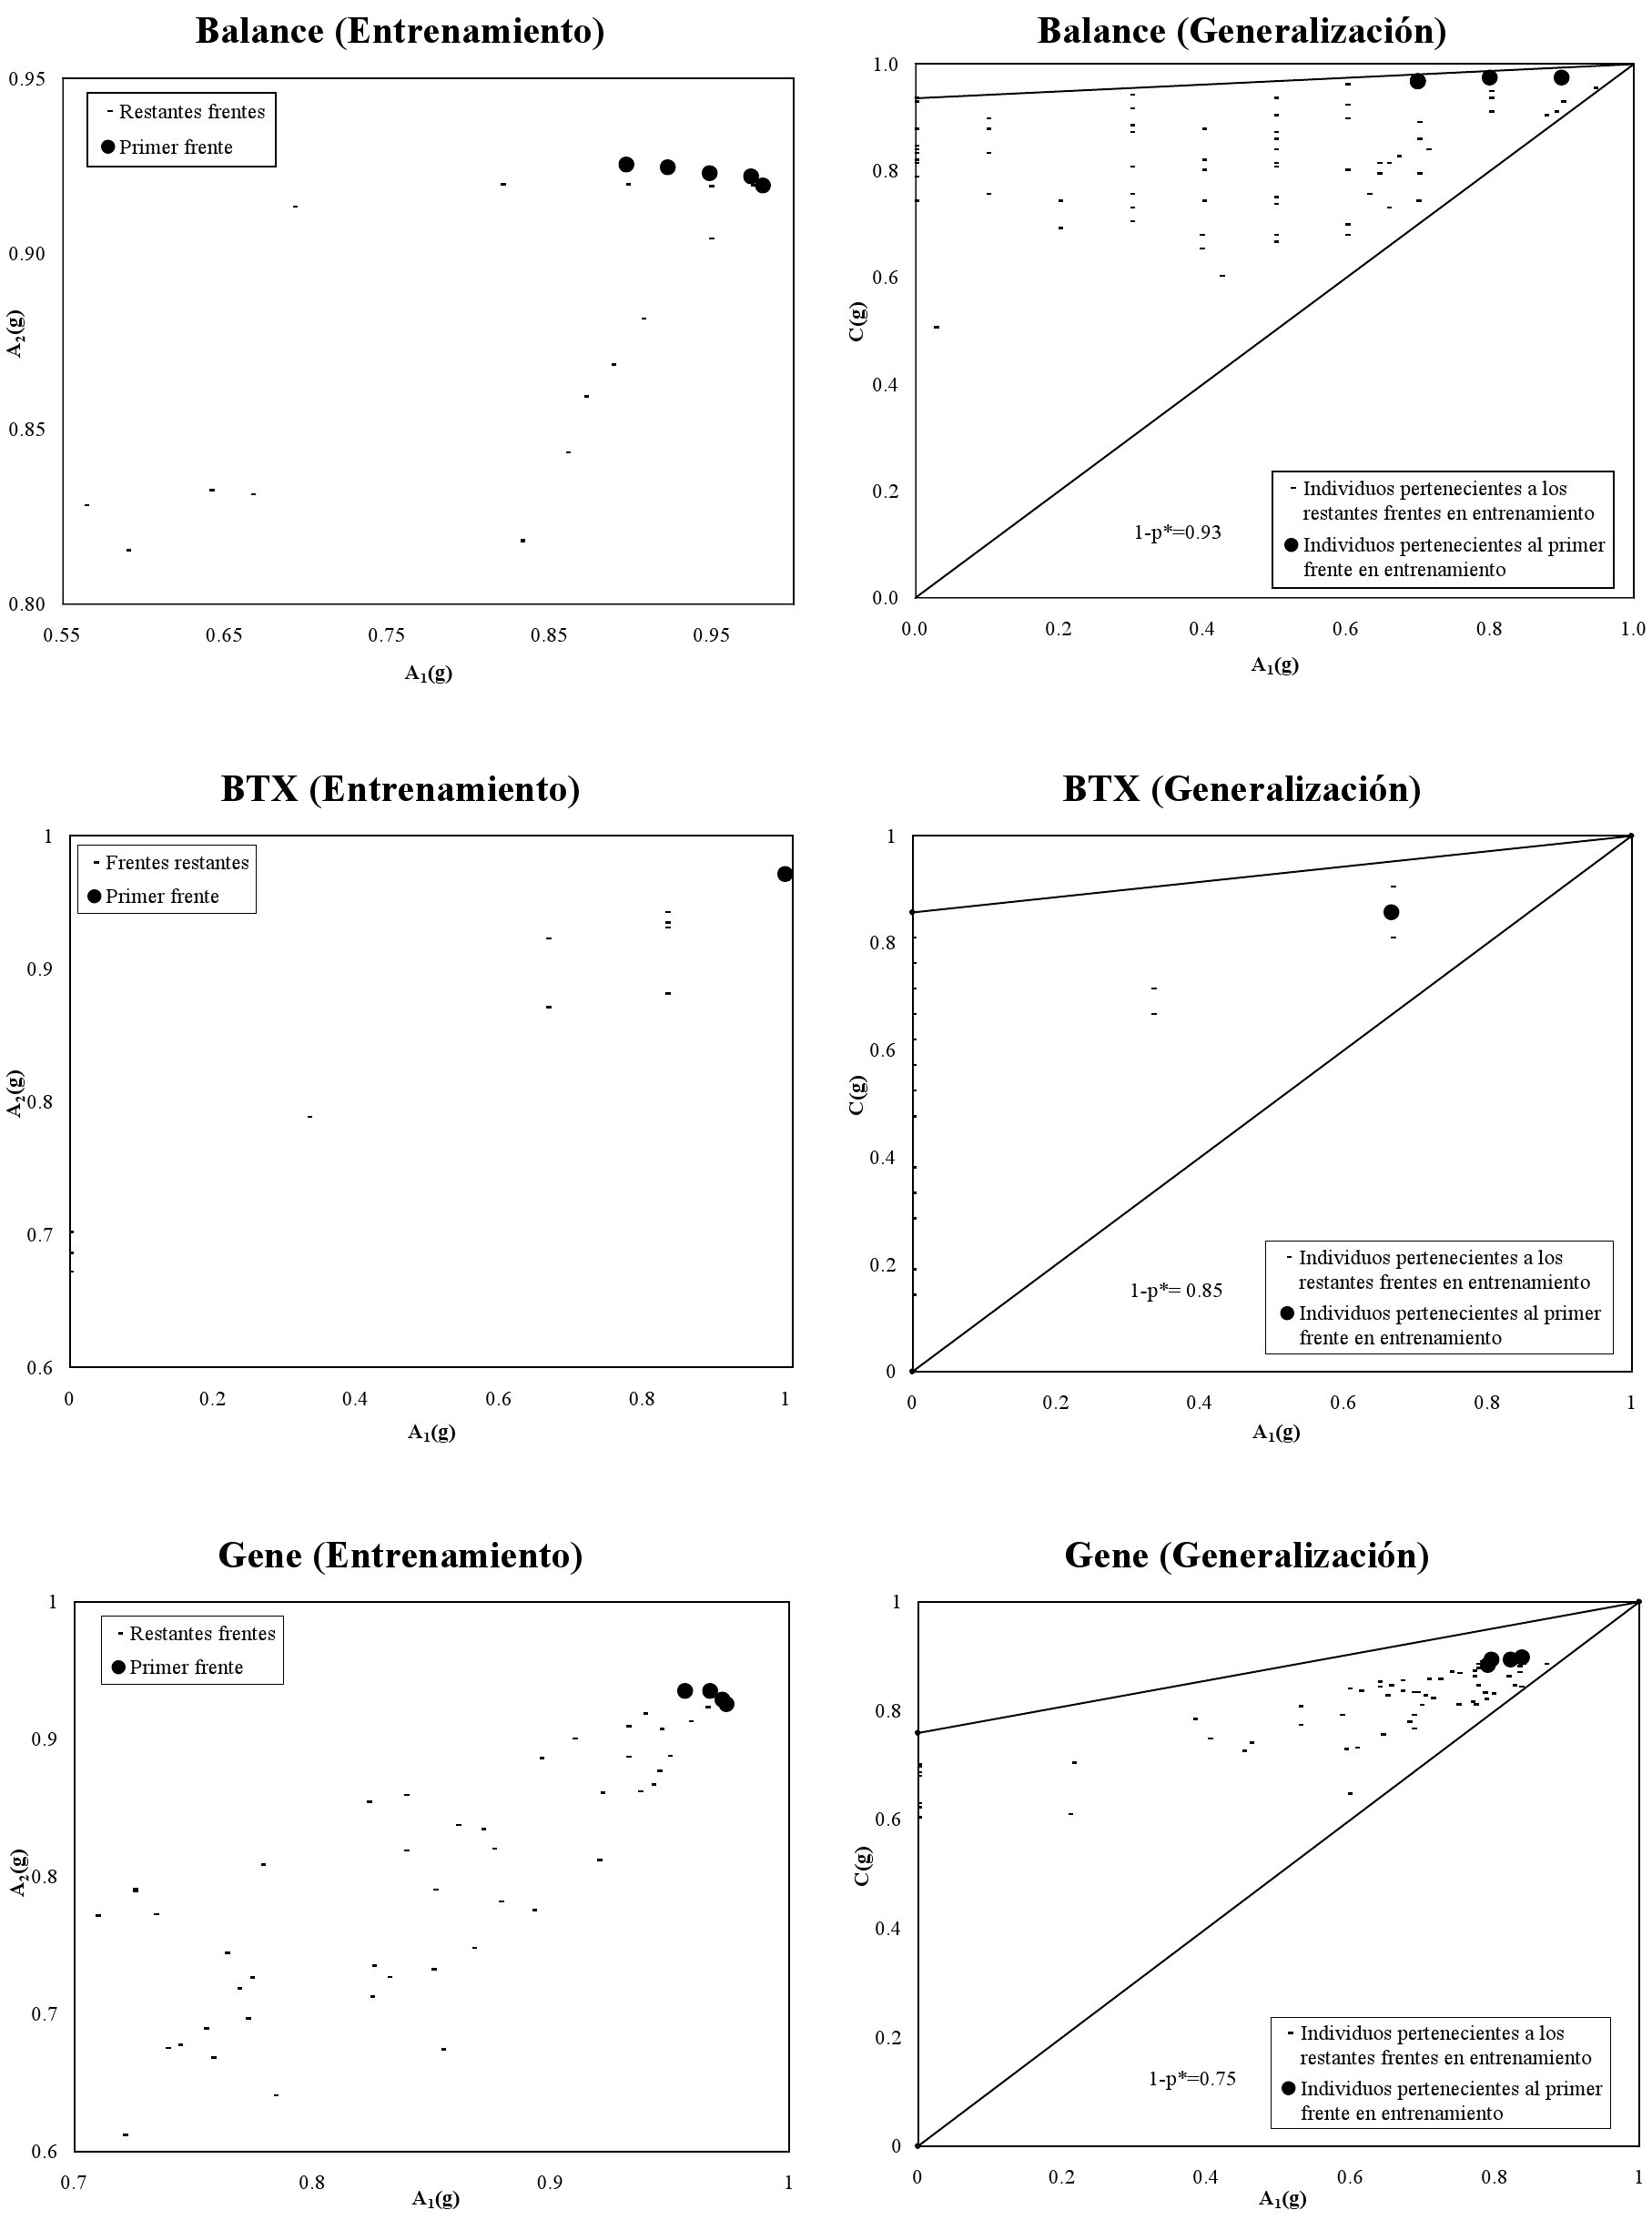
\includegraphics[keepaspectratio,width=13cm]{figuras/tanda4.jpg}
	\caption{Frente de Pareto en entrenamiento $(A_{1},A_{2})$, y valores asociados
a $(A_{1},C)$ en generalización para los conjuntos Balance, BTX y Gene.}
\label{tanda4}
\end{figure}

\begin{figure}[!htb]
\centering
	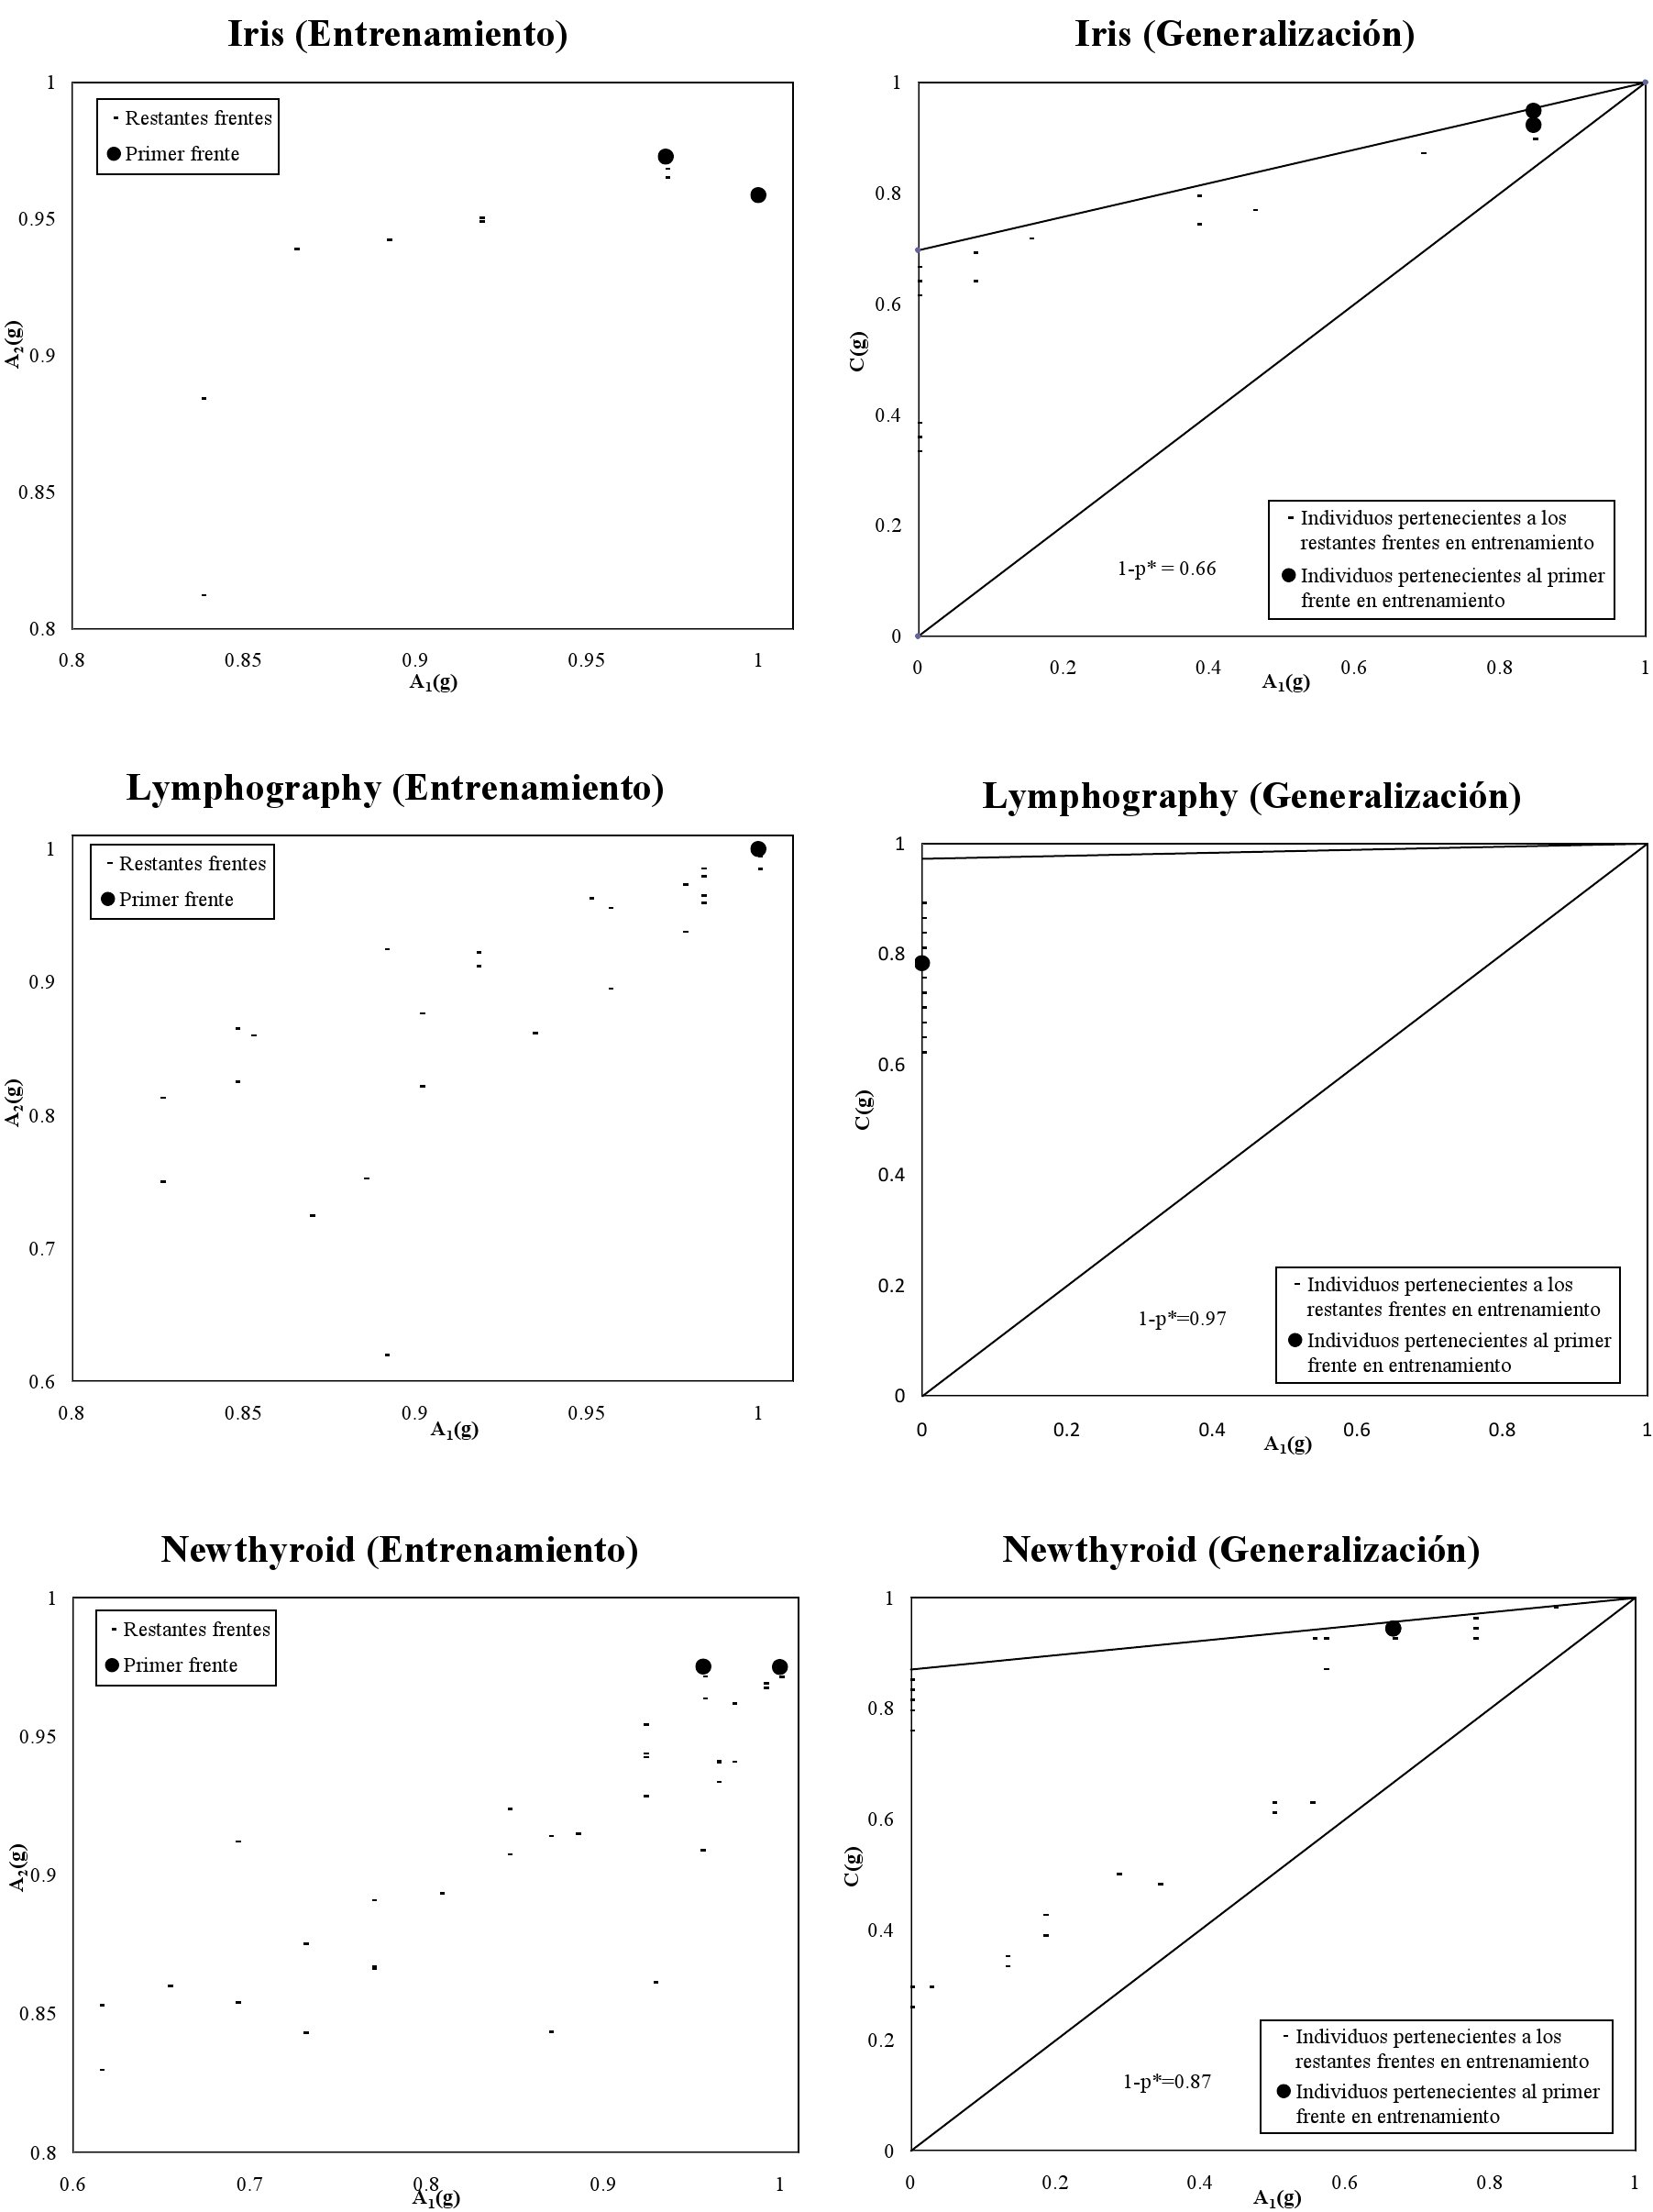
\includegraphics[keepaspectratio,width=13cm]{figuras/tanda5.jpg}
\caption{Frente de Pareto en entrenamiento $(A_{1},A_{2})$, y valores asociados a
$(A_{1},C)$ en generalización para los conjuntos Iris, Lymphography y Newthyroid.}
\label{tanda5}
\end{figure}

\begin{figure}[!htb]
\centering
	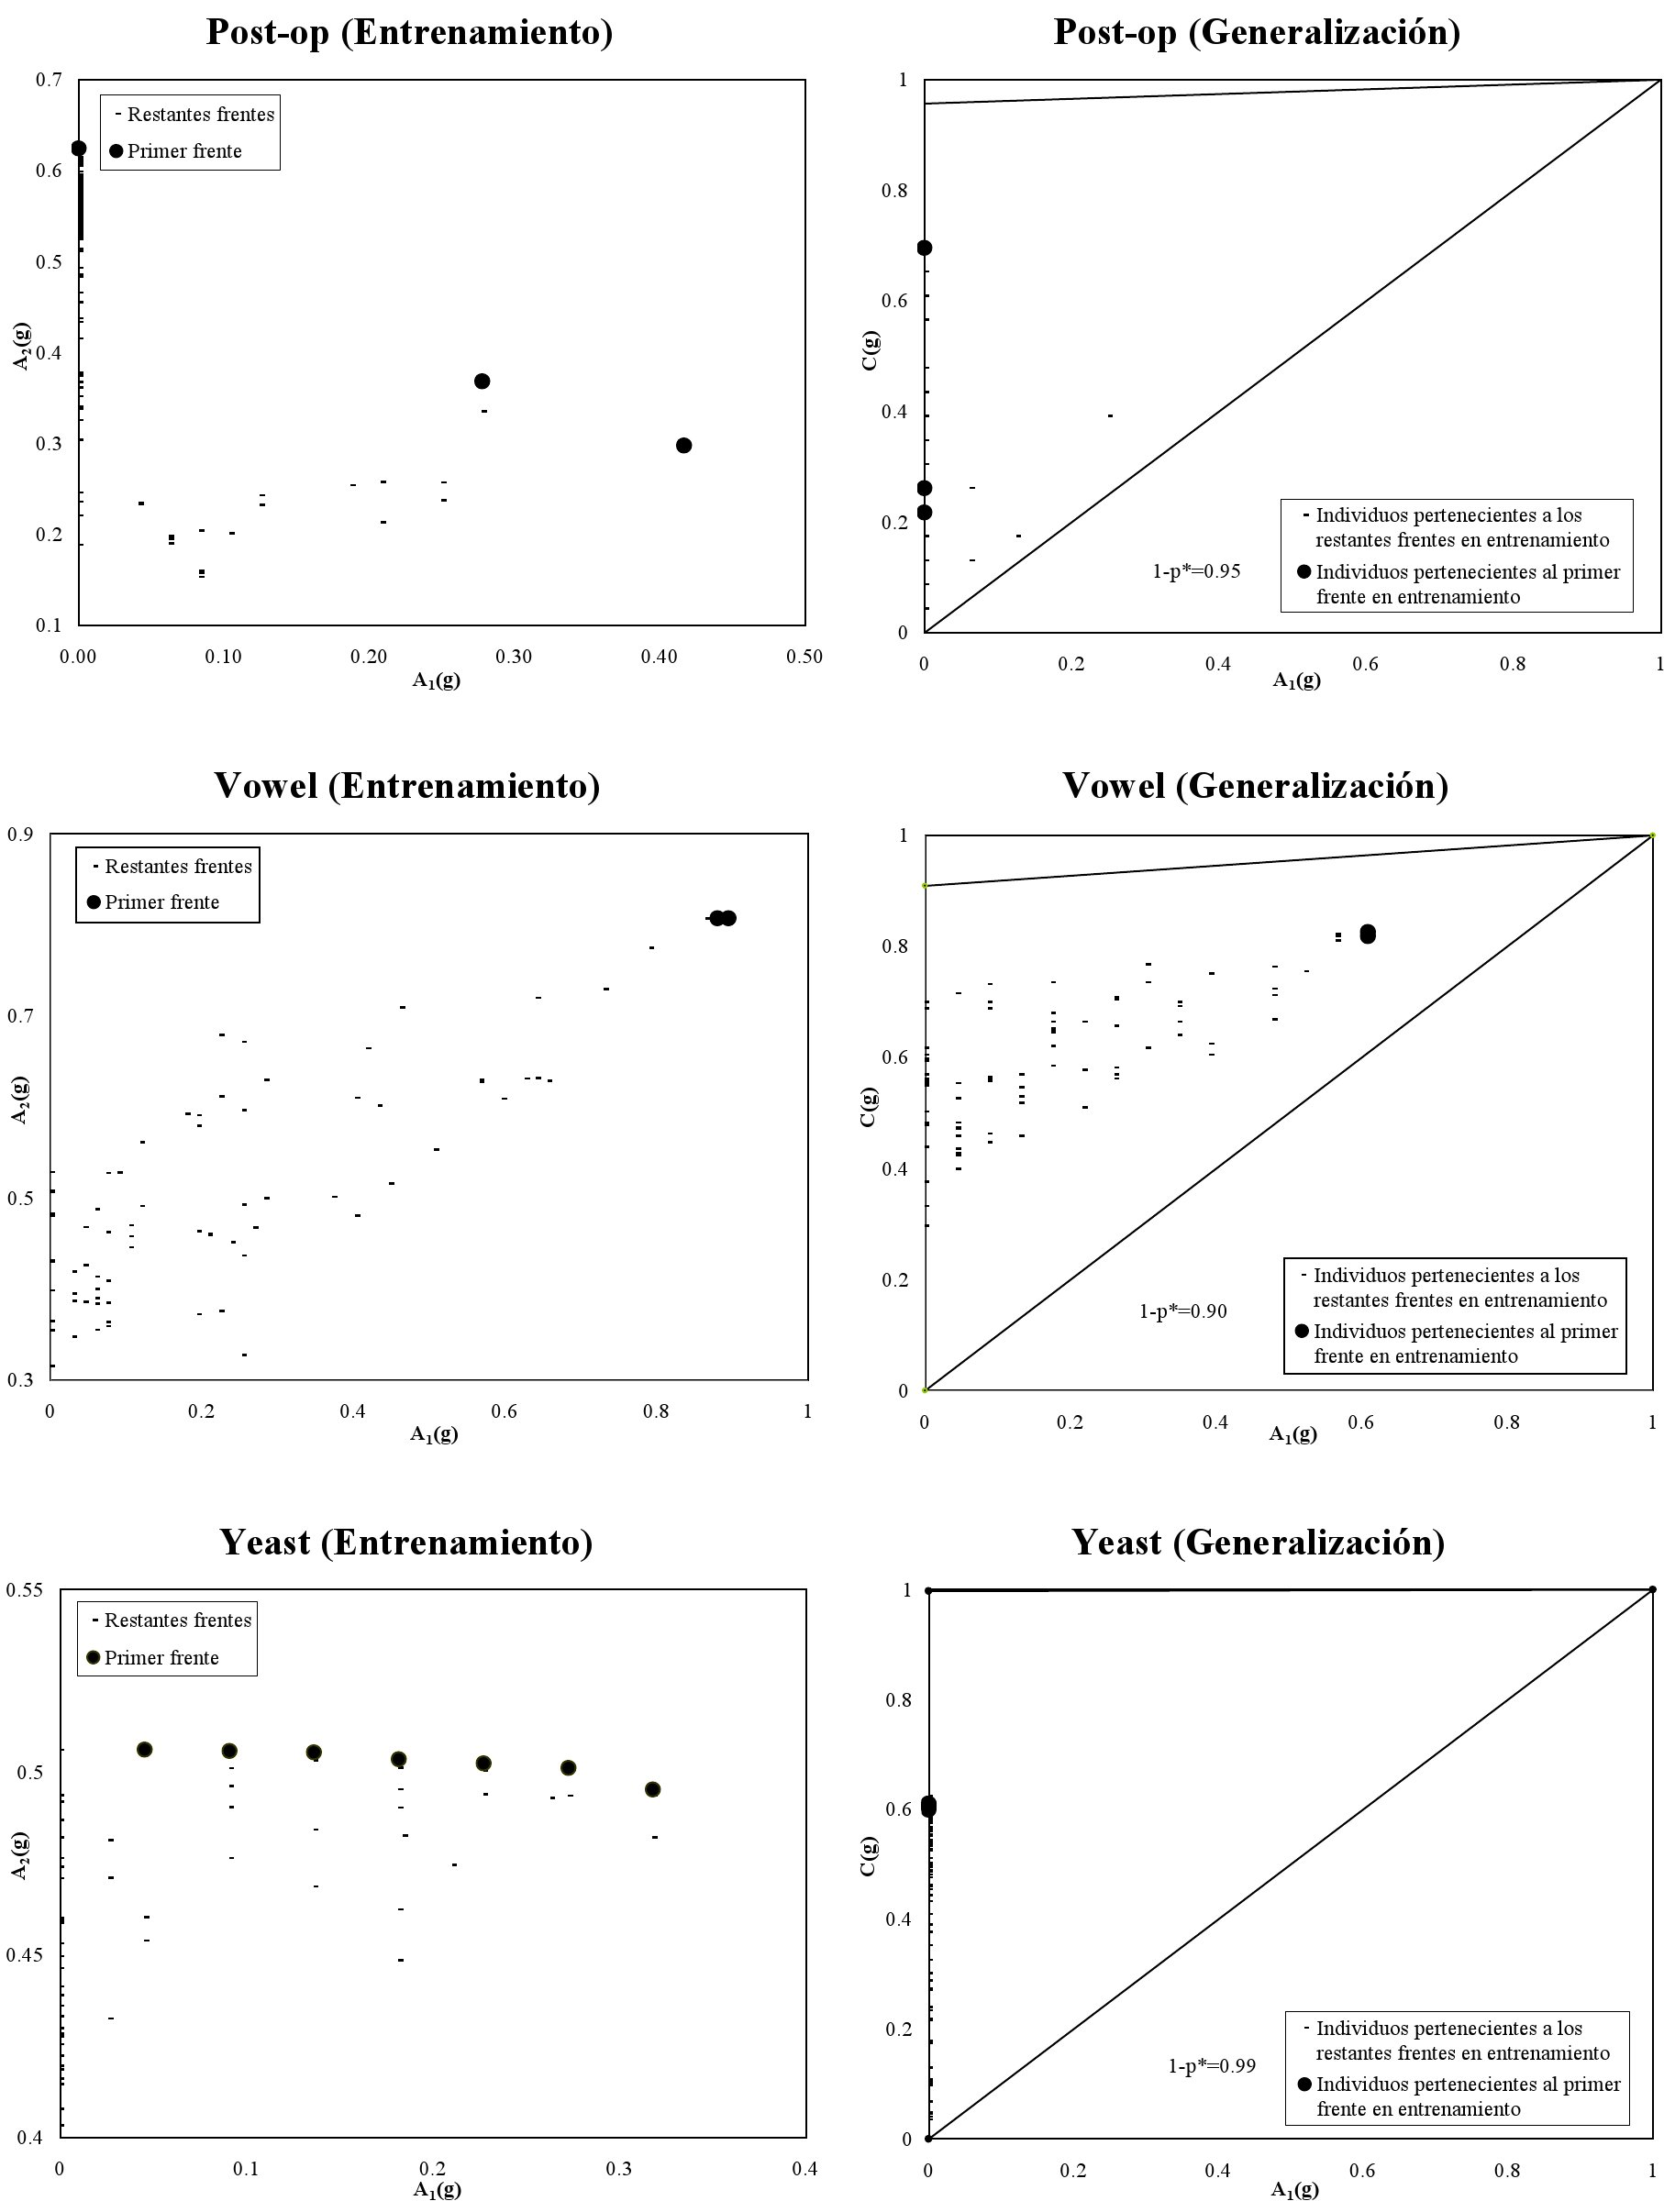
\includegraphics[keepaspectratio,width=13cm]{figuras/tanda6.jpg}
\caption{Frente de Pareto en entrenamiento $(A_{1},A_{2})$, y valores asociados a
$(A_{1},C)$ en generalización para los conjuntos Post-op, Vowel y Yeast.}
\label{tanda6}
\end{figure}

\clearpage
Finalmente, el lector puede observar en la figura \ref{ejemploPima}, como ejemplo, el
error
de $MS$ contra precisión para el algoritmo MPENSGAII en entrenamiento y
y en generalización, para el conjunto Pima. En dicha figura se puede ver
el frente de Pareto en entrenamiento y los valores asociados al plano $(MS,C)$ tanto en
entrenamiento como en generalización (en una de las 30 ejecuciones para ese
conjunto).

\begin{figure}[!htb]
\centering
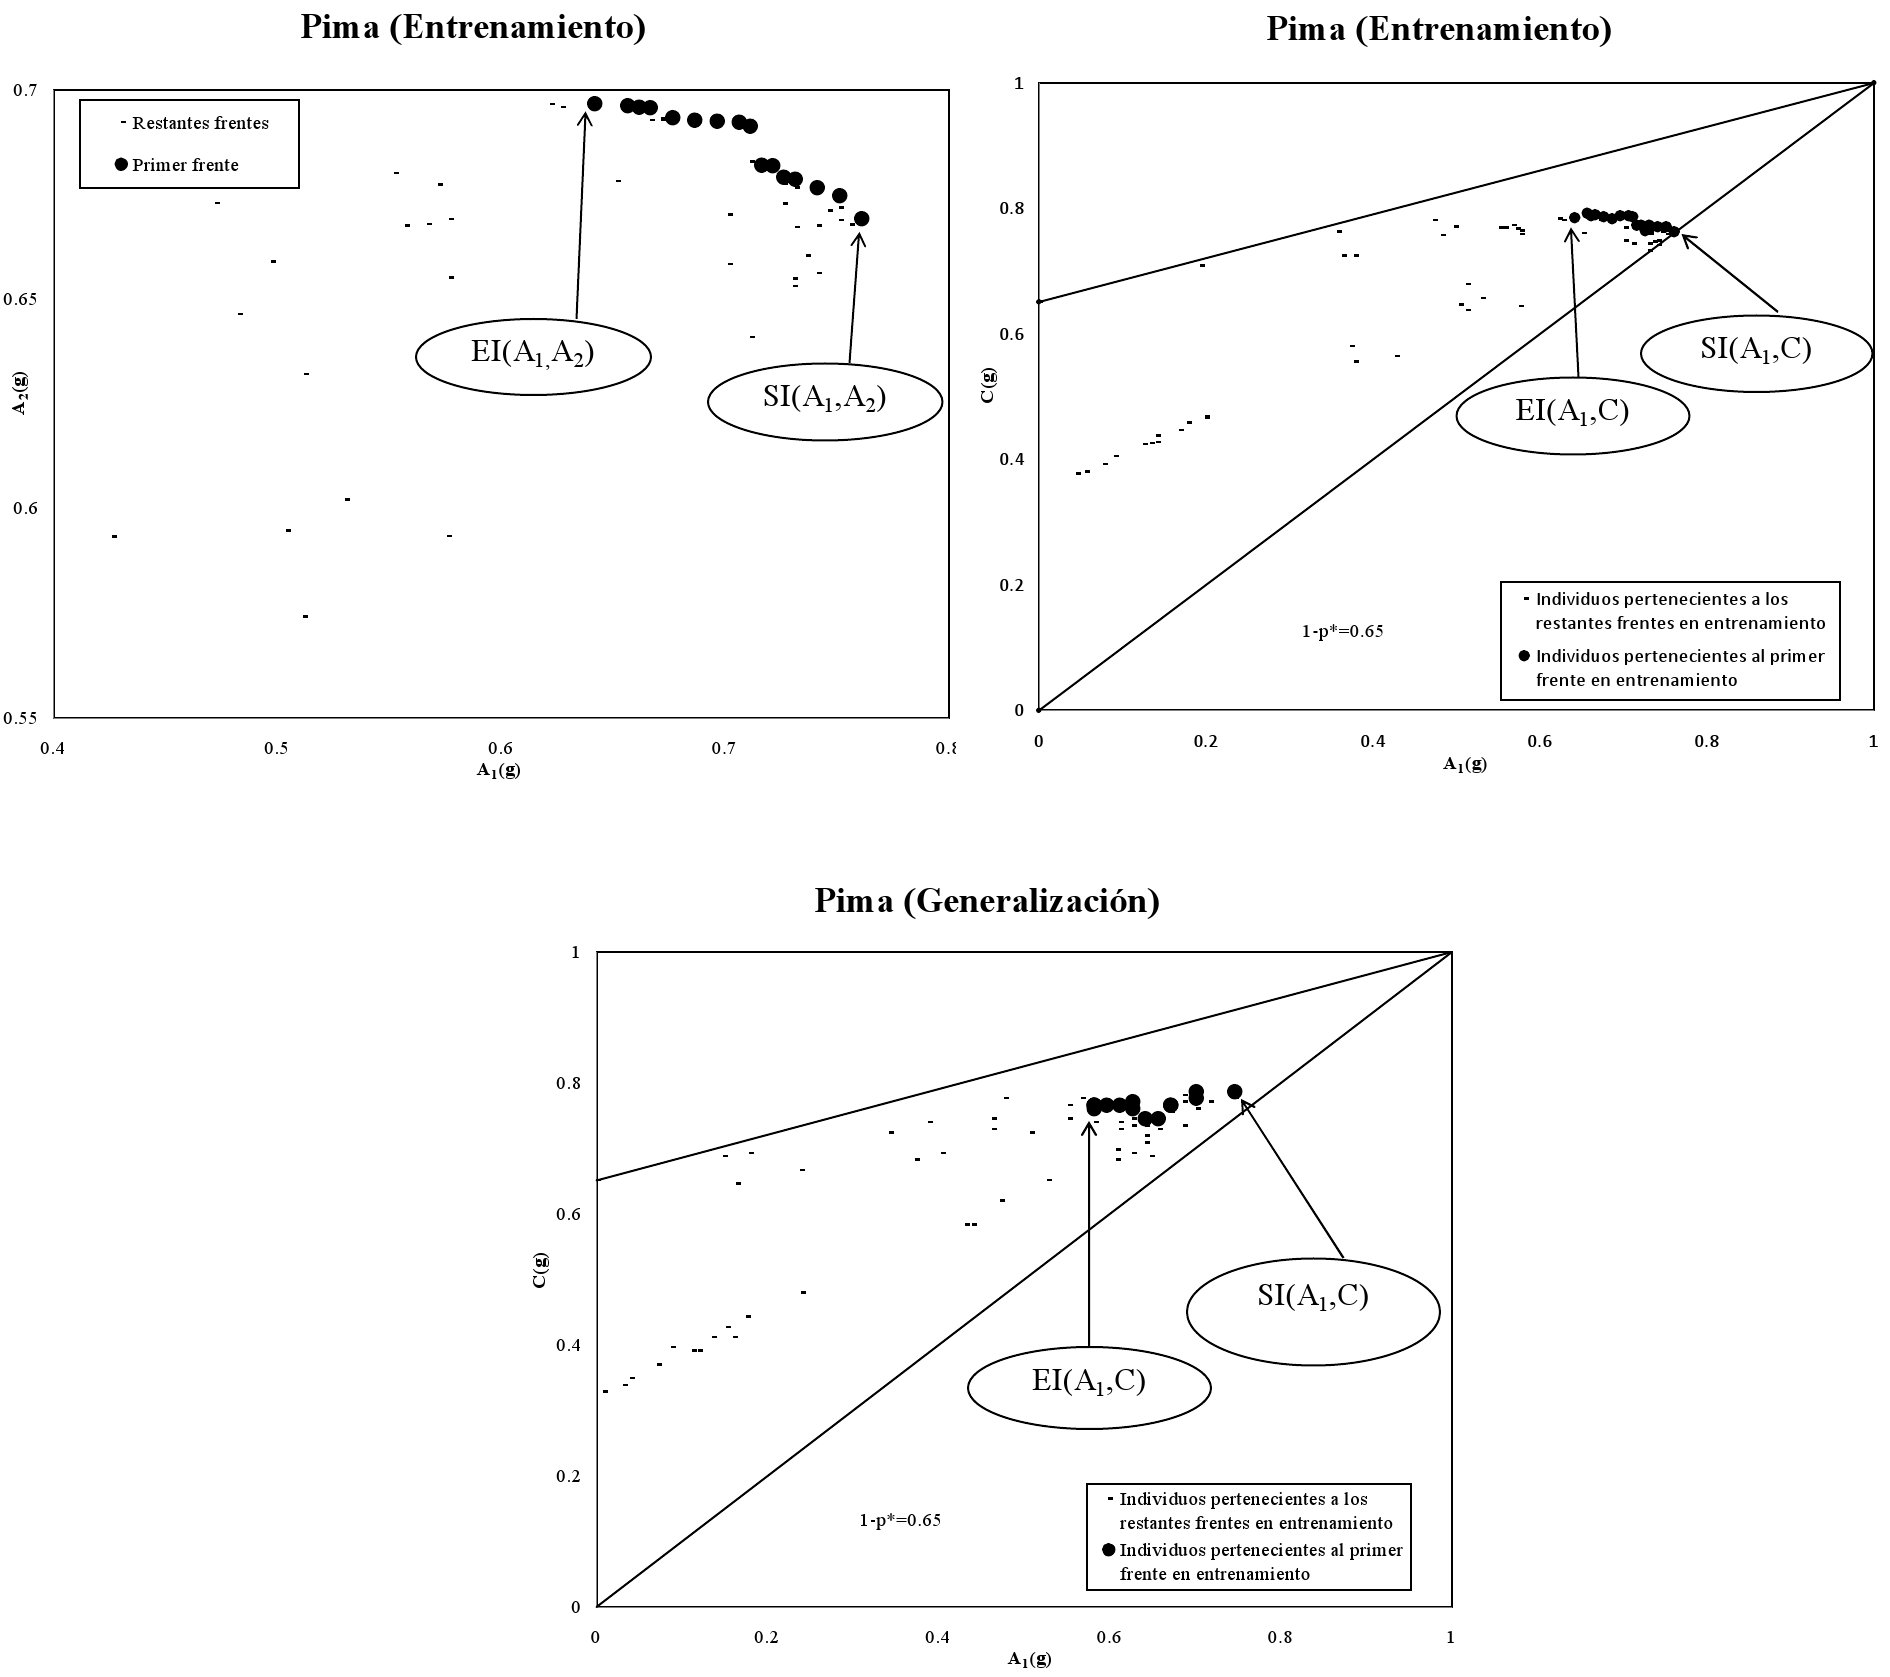
\includegraphics[keepaspectratio,width=13cm]{figuras/ejemploPima.jpg}
\caption{Ejemplo de frente de Pareto en entrenamiento $(A_{1},A_{2})$, y valores asociados
a $(A_{1},C)$ en entrenamiento y generalización para el conjunto Pima en una
ejecución
concreta.}
\label{ejemploPima}
\end{figure}
\newpage
En la tabla \ref{tabla5MPENSGAII} mostramos los mejores modelos que se han
obtenido en entrenamiento para Pima (extremos del frente de Pareto) junto con el número de
neuronas, número de enlaces, los valores $A_{1}$, $A_{2}$, $MS$ y $C$ en entrenamiento y
los valores $MS$ y $C$ en generalización, para una ejecución de las 30, que como
siempre es la que presenta el mejor individuo en $E$. Un punto a destacar sobre
estos modelos es que el algoritmo MPENSGAII poda las conexiones, seleccionando las
variables más importantes para la clasificación. El modelo MPENSGAIIE presenta mayor
número de variables de entrada que el modelo MPENSGAIIS, por lo que el número de
conexiones es mayor, 39 para el primero y 26 para el segundo, aunque ambos necesitan 4
neuronas en la capa intermedia. Como se puede observar, el valor de $A_{1}$ en
entrenamiento para MPENSGAIIE (0.64) es menor que para MPENSGAIIS (0.76), y justo al
contrario pasa con el valor de $A_{2}$, siendo 0.69 para MPENSGAIIE y 0.66 para
MPENSGAIIS. Con respecto a los valores de $MS$ en entrenamiento, el modelo
MPENSGAIIE tiene un valor de $MS$ de 0.64 mientras que el modelo MPENSGAIIS tiene un valor
de 0.76, ya que este último modelo es del extremo inferior del frente de Pareto. En
cuanto al valor de $C$ en entrenamiento, el modelo MPENSGAIIE tiene una valor de 0.78
frente a un valor de 0.76 del modelo MPENSGAIIS, ya el el modelo MPENSGAIIE es del
extremo superior del frente de Pareto. Finalmente en generalización el modelo MPENSGAIIS
obtiene mejores valores tanto en $MS$ como en $C$, por lo que en este caso recomendamos ésta
metodología, ya que presenta valores de $MS_{G}=0.74$, frente a $MS_{G}=0.58$ para MPENSGAIIE,
siendo estos valores en $C_{G}$ similares.

\begin{landscape}
\begin{table}[!htb]
\scriptsize
\tabcolsep 15pt
\caption{Mejores modelos en entrenamiento para Pima en los extremos
del primer frente de Pareto obtenido con MPENSGAII, con sus correspondientes valores en
generalización.}
\label{tabla5MPENSGAII}
\begin{tabular}{>{\columncolor[rgb]{0.86,0.94,1}}p{2.2cm}>{\columncolor[rgb]{0.86,0.94,1}}
l}\hline
\rowcolor[rgb]{0.70,0.85,1}\textbf{Individuo} & \textbf{Modelo matemático} \\ \hline
& $DF_{E}=2.74 - 4.74B_{1}(\bar{x},\Theta) + 4.81B_{2}(\bar{x},\Theta) -
1.09B_{3}(\bar{x},\Theta)+4.04B_{4}(\bar{x},\Theta)$ \\
& \\
& $B_{1}(\bar{x},\Theta)= (1/(1+\exp\left\lbrace
-(+1.07x_{1}+0.66x_{2}+0.43x_{3}-0.42x_{5}+5.89x{6}-2.92x_{7}+0.06x_{8}+0.69)
\right\rbrace))$\\
& $B_{2}(\bar{x},\Theta)= (1/(1+\exp\left\lbrace-(-0.17x_{1}-4.02x_{2}+1.07x_{3}+0.72x_{4}
+0.14x_{5}+1.22x_{6}-4.15x_{7}-2.96x_{8}-3.08)\right\rbrace))$ \\
& $B_{3}(\bar{x},\Theta)=
(1/(1+\exp\left\lbrace-(+0.62x_{1}+0.64x_{2}+0.24x_{3}-0.02x_{4}-0.02x_{5}+6.
22x_{6}+1.06x_{7}+0.07x_{8}+1.95)\right\rbrace))$ \\
& $B_{4}(\bar{x},\Theta)=
(1/(1+\exp\left\lbrace-(+0.70x_{1}-0.57x_{2}-0.57x_{3}-0.52x_{4}-1.08x_{5}-1.
87x_{6}+4.87x_{8}-2.84)\right\rbrace))$ \\
& \\
& $A_{1}(g)=0.64$; $A_{2}(g)=0.69$; $MS_{{\rm T}}=0.64$; $C_{{\rm T}}=0.78$; $MS_{{\rm
G}}=0.58$; $C_{{\rm G}}=0.76$;\\
\multirow{-8}{2.2cm}{Mejor individuo en el plano $(A_{1},A_{2})$ considerando $A_{2}$
(MPENSGA2E)}& neuronas = 4; conexiones efectivas = 39\\ \hline
& $DF_{MS}=2.77- 4.76B_{1}(\bar{x},\Theta) +
4.74B_{2}(\bar{x},\Theta)-1.09B_{3}(\bar{x},\Theta)+3.12B_{4}(\bar{x},\Theta)$\\
& \\
& $B_{1}(\bar{x},\Theta)=(1/(1+\exp\left\lbrace-(+4.41x_{6}-2.98x_{7}
+0.97(1))\right\rbrace))$\\
& $B_{2}(\bar{x},\Theta)=
(1/(1+\exp\left\lbrace-(+0.20x_{1}-4.73x_{2}+1.03x_{4}+0.10x_{5}-2.89x_{6}
-4.55x_{7}-3.27x_{8}-3.01(1))\right\rbrace))$ \\
& $B_{3}(\bar{x},\Theta)=(1/(1+\exp\left\lbrace-(-0.07x_{2}+0.13x_{4}+0.77x_{6}
+1.13x_{7}+0.07x_{8}+1.89(1))\right\rbrace))$\\
&$B_{4}(\bar{x},\Theta)=(1/(1+\exp\left\lbrace-(+0.24x_{1}-0.26x_{7}+6.69x_{8}
-2.66(1))\right\rbrace))$\\
& \\
& $A_{1} (g)=0.76$; $A_{2} (g)=0.66$; $MS_{{\rm T}}=0.76$; $C_{{\rm T}}=0.76$;
$MS_{{\rm G}}=0.74$; $C_{{\rm G}}=0.78$;\\
\multirow{-8}{2.2cm}{Mejor individuo en el plano $(A_{1},A_{2})$ considerando $A_{1}$
(MPENSGA2S)} & neuronas = 4; conexiones efectivas = 26\\ \hline
\multicolumn{2}{l}{DF=Función discriminante.}\\
\end{tabular}
\end{table}
\end{landscape}

A modo de resumen y conclusión, la metodología MPENSGAII propone una nueva aproximación
en problemas de clasificación multi-clase basada en una medida de rendimiento
bidimensional, $MS$ y $C$. Los resultados muestran
que con estas medidas es posible obtener clasificadores que combinen un nivel alto de
clasificación con un buen nivel de clasificación por clase.

Una de las áreas que mas auge ha tenido en los últimos años dentro del
aprendizaje automático es aquella en donde se combinan las decisiones de clasificadores
individuales, con la finalidad de que la decisión final de a qué clase pertenece un
ejemplo se realice por un conjunto de clasificadores, a los que se les suele
llamar \textit{ensemble} \cite{Dietterich1997,Kuncheva2005}.

\section{\textit{Ensembles} de clasificadores}\label{introEnsembles}
\noindent Cuando se habla de \textit{ensembles} es necesario distinguir entre: la manera
de generar clasificadores, la manera de elegir qué clasificadores de entre los que
disponemos y cuáles de ellos formarán el \textit{ensemble} (ligado al concepto de
diversidad),
y finalmente, las reglas o formas de utilizar el \textit{ensemble} para clasificar a un
determinado patrón o instancia. Dependiendo de lo que se tenga en cuenta, hay autores que
hacen una taxonomía de \textit{ensembles} diferente. El lector puede consultar un extenso
estado del arte, referencias bibliográficas y taxonomías para la formación de
\textit{ensembles} en tareas de clasificación en \cite{Rokach2009}.

Siguiendo el trabajo de Rokach \cite{Rokach2009}, los aspectos a
tener en cuenta en la creación de un \textit{ensemble} son:
\begin{description}
	\item[$\blacktriangleright$ Uso del combinador:] Se entiende por combinador al proceso
de combinar las
clasificaciones arrojadas por varios clasificadores que forman un \textit{ensemble} para
obtener una conclusión, decisión, o clasificación final.

Existen, de manera general, dos métodos de combinación:
\begin{enumerate}
	\item \textbf{Métodos de pesos o de ponderación:} Estos métodos son más adecuados para
problemas en los que cada uno de los clasificadores realizan la misma tarea y tienen un
éxito equiparable, o cuando nos gustaría evitar problemas asociados al sobre-aprendizaje.
Suelen utilizar ponderaciones de las probabilidades de salida o de las asignaciones que
realiza cada clasificador a un determinado patrón para obtener la decisión final. Ejemplos
de esté tipo de técnicas (ver \cite{Rokach2009}) son: la mayoría de votos
(\textit{Majority
Voting}), la ponderación por rendimiento (\textit{Performance Weighting}), la distribución
de sumas o media simple (\textit{Distribution Summation} or \textit{Simple Averaging}), el
ganador lo consigue todo (\textit{Winner Takes All}) \cite{Theodoridis2006} (esta último
método no se cuentra en \cite{Rokach2009}), el método de \textit{Dempster-Shafer}, o el
método de
Naive Bayes.

	\item \textbf{Métodos de meta-aprendizaje:} Los métodos de meta-aprendizaje son más
convenientes para casos en los que determinados clasificadores cometen
errores de manera consistente en determinadas instancias. El aprendizaje se produce a
partir de los clasificadores inducidos y a partir de las clasificaciones de éstos
clasificadores en el conjunto de entrenamiento. Es decir, de alguna manera se introduce
un meta-aprendizaje a partir de los resultados que proporcionan algunos clasificadores
del \textit{ensemble} para proporcionárselos a otros, utilizando o no divisiones del
conjunto de entrenamiento inicial o mediante combinación de éste con las salidas de
clasificadores previos. Suele hacerse un aprendizaje por etapas. Ejemplos de estos
métodos (ver \cite{Rokach2009}) son \textit{Stacking}, \textit{Arbiter Trees},
\textit{Combiner Trees}, \textit{Grading}, \textit{Adaptive fusion and co-operative
training} y \textit{Mathematical Programming}.

La mayoría de los métodos de combinación no tienen en cuenta si los clasificadores son
dependientes o independientes (detallado a continuación). De esta manera, cuando los
clasificadores son dependientes, el rendimiento de los métodos de combinación se degrada,
sugiriéndose en la literatura varias técnicas para evitar el descenso de rendimiento
\cite{Rokach2009}, como por ejemplo transformar las salidas de los clasificadores a
medidas de confianza, de forma tal que cada transformación sea la combinación de una
función escalar y de un tipo de confianza \cite{Liu2005}.
\end{enumerate}
\item[$\blacktriangleright$ Dependencia de los clasificadores:] Se refiere a la manera
en la que se entrenan
los clasificadores que formarán un \textit{ensemble}, y de cómo un clasificador puede
afectar a otro en la decisión final. Así, los clasificadores pueden ser dependientes
o independientes.

En un marco \textbf{dependiente}, el resultado de un clasificador afecta a la
creación del siguiente, de manera que hay interacción en el proceso de aprendizaje. De
esta manera se puede utilizar el conocimiento generado en iteraciones previas para guiar
el aprendizaje de futuras iteraciones. Hay dos aproximaciones \cite{Rokach2009} relacionas
con la creación de clasificadores dependientes:
\begin{enumerate}
\item \textbf{Modelos guiados por selección de instancias:} En esta aproximación
los clasificadores se construyen mediante una serie de iteraciones previas, las cuales se
utilizan para cambiar el conjunto de entrenamiento para las siguientes iteraciones.
Estos métodos suelen ignorar las instancias que están bien clasificadas por los
clasificadores en pasos anteriores. Un ejemplo de este tipo de métodos, a los que se les
suelen llamar métodos de \textit{Boosting} (también se nombran por métodos de
\textit{Resampling} o \textit{Combining}), es el algoritmo AdaBoost y su
multitud de variantes \cite{Rokach2009}.
\item \textbf{Aprendizaje incremental por lotes:} Los métodos de aprendizaje incremental
utilizan la clasificación de iteraciones previas como conocimiento ``a priori'' para el
algoritmo de aprendizaje en la siguiente iteración. Dicho algoritmo utiliza el conjunto
actual de entrenamiento junto con la clasificación del clasificador formado para la
construcción del siguiente clasificador. El clasificador construido en la última iteración
se elige como clasificador final.
\end{enumerate}

En un marco \textbf{independiente}, el conjunto de datos original se particiona en varios
subconjuntos, a partir de los cuales se obtendrán varios clasificadores. El conjunto de
datos de entrenamiento original debe ser inconexo (mutuamente excluyente) o superpuesto.
Como el proceso por el cual se obtienen los datos o resultados finales a partir de la
combinación de varios clasificadores es independiente del algoritmo de aprendizaje
utilizado, se pueden utilizar diferentes clasificadores de manera paralela, disminuyendo
el tiempo de cómputo. El método independiente más popular es el método de \textit{Bagging}
\cite{Breiman1996} y sus variantes \cite{Rokach2009}, que se  basa en el submuestreo con
reemplazamiento del conjunto de entrenamiento para generar un grupo diferente de
hipótesis,
utilizando cada muestra obtenida como un conjunto de entrenamiento diferente para generar
un clasificador. Al utilizarse el reemplazo puede haber instancias o patrones repetidos en
varios conjuntos de entrenamiento, por lo que desde el punto de vista estadístico puede
haber una cierta dependencia. El clasificador resultante suele utilizar el método de la
mayoría de votos (\textit{Majority Voting}) \cite{Theodoridis2006}, basándose en la salida
de cada uno de los clasificadores que forman el \textit{ensemble}. Se pueden
consultar otros métodos como \textit{Random Forest Ensemble} o \textit{Cross-validate
Committees} en \cite{Rokach2009}.
\item[$\blacktriangleright$ Diversidad del generador:] Se refiere a la manera en la que el
algoritmo de
aprendizaje o método que se utilice para producir clasificadores proporciona diversidad
\cite{Chandra2006,Kuncheva2005,Chandra2004,Chandra2006b}. Se considera que dos
clasificadores son diversos, si los errores que cometen sobre los datos de entrada no
están correlados.

Un \textit{ensemble} debería tener estas dos características: diversidad y precisión. Es
importante que los modelos que forman un \textit{ensemble} sean buenos en cuanto a
precisión, pero
también es necesario que sean diversos, es decir, que el conjunto de individuos que lo
conforman no sean similares entre si y que unos posean características que otros no
tengan. El concepto de equilibrio precisión-diversidad se refiere a
cómo la diversidad de los individuos contribuye a mejorar la precisión del
\textit{ensemble}, y de cómo el rendimiento de un elemento del \textit{ensemble} puede
afectar al conjunto \cite{Chandra2004}. En otras palabras, si se tiene una mayor
diversidad en el \textit{ensemble}, la precisión del decisor final, en general,
aumentará. De forma general, se pueden usar varias técnicas a la
hora de obtener frentes diversos y precisos \cite{Rokach2009,Brown2005,Sharkey1999}:
Diferentes presentaciones de los datos de entrada, variaciones en el diseño del
clasificador/es, entrenamiento individual, secuencial o simultaneo de los clasificadores,
adición de penalización a las salidas, manipulación del conjunto de entrenamiento y de la
arquitectura de las ANNs.

En el contexto de regresión, el concepto de equilibrio precisión-diversidad se
explica mediante la descomposición sesgo-varianza-covarianza, sin embargo, en el contexto
de clasificación no hay una teoría o acuerdo sobre cómo la precisión y la diversidad
influyen una sobre la otra \cite{Brown2005}, de manera que hay diferencia de opiniones en
cuanto a una descomposición varianza-covarianza.

En \cite{Chandra2004} se hace una descomposición sesgo-varianza-covarianza atendiendo al
error cuadrático de un \textit{ensemble} de clasificadores de ANNs, de manera que dicho
error depende del sesgo, de la varianza y también de la relación entre los individuos que
forman el conjunto de clasificadores. También se utiliza esta descomposición para
explicar la sensibilidad del error cuadrático de un \textit{ensemble} a través de la
covarianza (en las salidas estimadas) entre los distintos individuos o redes.	El término
covarianza se utiliza para indicar la diversidad entre los miembros del \textit{ensemble}.
Se cree que cuanto más diversos sean los miembros individuales del conjunto, estarán
menos correlados. Esto sugiere que la covarianza de las salidas debe de ser lo más baja
posible. Cuanto menor sea la covarianza, menor será el error de correlación
entre las redes, lo que implica reducción de errores y un mejor rendimiento a nivel de
conjunto. Esta es la razón principal por la que la diversidad en \textit{ensembles} es
extremadamente importante.

Brown en \cite{Brown2005} hace una revisión de las técnicas de diversidad en
\textit{ensembles} y sugiere una nueva taxonomía de métodos:
\begin{enumerate}
	\item \textbf{Punto de comienzo en el espacio de búsqueda:} Este método varia los
puntos de inicio dentro del espacio de búsqueda, lo que influye hacia dónde se
converge en dicho espacio.
   \item \textbf{Conjunto de espacios de búsqueda accesibles:} Este método varía el
conjunto de espacios de búsqueda que son accesibles por el \textit{ensemble}. Teniendo
en	cuenta que ciertos espacios de búsqueda pueden ser accesibles o inaccesibles con un
		subconjunto particular de entrenamiento, o por la arquitectura de algunos elementos
		del \textit{ensemble}, estas técnicas, o bien varían los datos de entrenamiento
		usados, o la arquitectura empleada por diferentes miembros del conjunto.
	\item \textbf{Recorrido del espacio de búsqueda:} Este método altera la forma en que
se atraviesa el espacio de búsqueda, lo que daría lugar a diferentes redes para converger
a diferentes espacios de búsqueda.
\end{enumerate}

En \cite{Rokach2009} se propone la siguiente taxonomía:
\begin{enumerate}
\item \textbf{Manipulación del inductor:} Se refiere a la manera en la que se usa el
inductor base o algoritmo de aprendizaje. Más específicamente, cada elemento del
\textit{ensemble} se entrena con un algoritmo de aprendizaje que se ha desarrollado de
manera diferente.
\item \textbf{Manipulación del conjunto de entrenamiento:} Aquí se varía el conjunto de
entrenamiento que utiliza el algoritmo de clasificación. Cada elemento del
\textit{ensemble} se entrena con un conjunto de datos diferente.
\item \textbf{Cambio en la representación de los atributos:} A cada clasificador del
\textit{ensemble} se le plantea un objetivo diferente, basándose en los
conceptos de agregación o descomposición del problema, por ejemplo, dividir un problema de
clasificación de $Q$
clases en $Q(Q-1)/2$ problemas binarios, donde cada problema considera la discriminación
de una clase frente a cada una de las restantes.
\item \textbf{Particionamiento del espacio de búsqueda:} Cada miembro del
\textit{ensemble} se entrena en un sub-espacio de búsqueda diferente.
\item \textbf{Hibridación:} La diversidad se obtiene usando varios algoritmos de
aprendizaje, o incluso varias estrategias de	decisión del \textit{ensemble}.
\end{enumerate}
\item[$\blacktriangleright$ Tamaño del ensemble:] Es importante determinar el número de
elementos que
forman el \textit{ensemble} y aquellos que hay que rechazar. Si el número de elementos
es demasiado pequeño, puede que el \textit{ensemble} no generalice demasiado bien, y si
el número de elementos es demasiado grande puede deteriorarse el rendimiento del decisor
si hay sobre-entrenamiento, y el coste computacional de entrenamiento aumenta. Hay varios
factores que son determinantes y que hay que tener en cuenta para decidir el tamaño
de un \textit{ensemble} \cite{Rokach2009}:
\begin{itemize}
\item Precisión deseada: Debe haber un equilibrio entre el número de elementos y la
precisión final, de manera que el número de elementos del \textit{ensemble} sea lo
suficientemente alto para reducir el error de clasificación.
\item Coste computacional: Incrementar el número de elementos normalmente incrementa
el coste computacional y disminuye su comprensibilidad.
\item Naturaleza del problema de clasificación: El tamaño del \textit{ensemble} puede
ser mayor o menor dependiendo de la naturaleza del problema.
\item Número de procesadores disponibles: Si se dispone de un número amplio de
procesadores para realizar una computación paralela, entonces es más flexible el tamaño que podemos
utilizar en el \textit{ensemble}.
\end{itemize}
Hay tres aproximaciones para determinar el tamaño de un \textit{ensemble}:
\begin{enumerate}
\item \textbf{Preselección del tamaño:} El tamaño del \textit{ensemble} se puede
determinar ``a priori'' con algún parámetro de configuración del algoritmo, o si tenemos
en cuenta la naturaleza del problema, haciendo un diseño previo dependiendo del
número de clases que tenga.
	\item \textbf{Selección del tamaño mientras se entrena:} Hay algoritmos que van
calculando el tamaño del \textit{ensemble} mientras se entrena y van comprobando si la
adición de un clasificador más mejora resultados anteriores, en caso contrario el
algoritmo deja de introducir clasificadores. También se puede establecer un límite
superior del tamaño del \textit{ensemble}
mediante algún parámetro de control.
	\item \textbf{Poda o post-selección del tamaño:} Consiste en dejar que el algoritmo de
aprendizaje o metodología que estemos usando cree tantos elementos del \textit{ensemble}
como sean necesarios. Una vez finalizado el proceso se pasa a un procedimiento de poda en
el que se van eliminando elementos del \textit{ensemble}, mientras no se reduzca de manera
importante la precisión del clasificador o decisor final. La poda de un \textit{ensemble}
no tiene porqué influir en su precisión y en su diversidad \cite{Liu2004}. Hay dos maneras
de podar un \textit{ensemble}, antes de realizar el proceso de combinación, por ejemplo
utilizando técnicas de validación o de diversidad, o después, donde se eliminan elementos
en función de su aporte al clasificador final, usando métricas como el rendimiento ROC
(ver capítulo \ref{medidasRendimiento}), algoritmos de selección de características
aplicados a los miembros del \textit{ensemble}, etc.
\end{enumerate}
\item[$\blacktriangleright$ Inductor cruzado:] Se refiere a la relación entre la técnica
de \textit{ensemble} y
el algoritmo de aprendizaje utilizado. En ocasiones la forma en la que se genera el
\textit{ensemble} depende del algoritmo de aprendizaje utilizado, es decir, es un único
proceso embebido donde hay una dependencia total. En otras ocasiones son independientes,
no teniendo que tener en cuenta qué método se ha usado para crear los clasificadores
cuando se hace una combinación de ellos.
\end{description}
% El lector puede ver una completa taxonomía sobre los aspectos a tener en cuenta a la
% hora de crear un ensemble en la figura 1 de \cite{Rokach2009}.

\subsection{\textit{Ensembles} con MOEAs}\label{ensemblesMOEAS}
\noindent Además de las técnicas descritas, es necesario comentar cómo se generan
\textit{ensembles} cuando se utilizan MOEAs basados en frente de Pareto, como en el caso
de MPENSGAII, ya que debido a la presencia de múltiples objetivos en conflicto, el
enfoque evolutivo genera un conjunto de soluciones cercanas a las soluciones óptimas, de
manera que se podría generar automáticamente un \textit{ensemble} donde los miembros
serían ANNs que estarían cercanas al óptimo \cite{Chandra2004}.

La principal razón para usar un enfoque evolutivo multi-objetivo para el diseño de
\textit{ensembles} es que la multi-objetividad refuerza el proceso de
búsqueda-optimización (siendo el proceso de búsqueda encontrar ANNs con un buen
rendimiento), obteniendo un conjunto de soluciones cercanas a las óptimas, en lugar de
sólo una única solución. Durante el proceso de obtención de un frente de Pareto de ANNs,
podríamos utilizar los individuos que se van obteniendo de manera automática en dicho
frente, como miembros de un \textit{ensemble}, el cual, como toda la población, con el
paso del tiempo avanzará hacia soluciones más prometedoras. Sin embargo, se plantea el
siguiente problema, (tal y como se comentó en la sección \ref{introEnsembles}, donde se
explicaba el concepto de diversidad en \textit{ensembles}), y es que si la
formulación del problema de optimización multi-objetivo hace que se obtengan individuos
con un buen rendimiento pero que no sean lo suficientemente diversos, posiblemente el
rendimiento del decisor final no sea tan bueno como esperamos. Por tanto, para que la
optimización multi-objetivo sea eficaz, el proceso de optimización debe conducir a la
convergencia hacia el frente de Pareto óptimo y al mismo tiempo se debe mantener una
distribución de soluciones en el frente de Pareto tan diversa como sea posible
\cite{Brown2004,Brown2005,Chandra2006b}.

En \cite{Abbass2001,Abbass2003b} se propone el algoritmo MPANN (Memetic Pareto
Artificial Neural Networks) para la construcción
de \textit{ensembles} con ANNs, basándose en DE.
Con MPANN se realiza una división del conjunto de entrenamiento en dos subconjuntos para
la obtención de diversidad, en los cuales hay que minimizar el $MSE$
como objetivo del proceso evolutivo, quedando formado el \textit{ensemble} con el
frente de Pareto de la última generación de la evolución.

En \cite{Chandra2006,Chandra2004} se propone DIVACE (\textit{DIVerse and ACcurate Ensemble
learning algorithm}), el cual usa las ideas del aprendizaje mediante
correlación negativa (\textit{Negative Correlation Learning}, NCL) de Liu \cite{Liu1999}
para la
obtención de diversidad, y del método MPANN de Abbass \cite{Abbass2001,Abbass2003b} para
la obtención de varios individuos precisos, minimizando el $MSE$, de manera que el
aprendizaje se formula como un problema multi-objetivo dentro de un marco
evolutivo que pretende encontrar un equilibrio entre precisión y diversidad. También se
escogen para el \textit{ensemble} todos los individuos del frente de Pareto generados
automáticamente con DIVACE.

En \cite{Islam2003} se propone un algoritmo para
el entrenamiento cooperativo de \textit{ensembles} de ANNs, utilizando para la obtención
de la
precisión un proceso constructivo automático que actúa sobre el número de neuronas en capa
oculta de las ANNs, y para la diversidad, el coeficiente de correlación negativa o NCL y
un entrenamiento especial por épocas para algunas ANNs de la población \cite{Liu1999}.
Con respecto al tamaño del \textit{ensemble}, se determina automáticamente en función
del error producido por los individuos que lo componen, y en función del número de
neuronas que tenga cada uno de ellos.

En \cite{Jin2004} se propone un MOEA basado en término de regularización mediante la
adición de un término en la función de coste del algoritmo de aprendizaje, obteniéndose
diferentes individuos en una sola ejecución. La selección de individuos para el
\textit{ensemble} se hace de dos formas: se escogen todos los individuos obtenidos en el
proceso de aprendizaje o solo algunos, en este último caso sin ninguna heurística
especial, solamente se tiene en cuenta que los individuos seleccionados se encuentren
distribuidos por todo el frente de Pareto.

En \cite{Pedrajas2005} se propone un marco de trabajo para generar \textit{ensembles} de
ANNs mediante coevolución cooperativa, usando ésta última para introducir diversidad, sin
usar términos que puedan sesgar el proceso de aprendizaje y la mejora colaborativa de las
redes. También se utilizan varias medidas de diversidad y de precisión durante el proceso
evolutivo para mantener el equilibrio del \textit{ensemble} entre ambas. Se usa un
MOEA donde evolucionan varios subconjuntos de ANNs, así como las mejores
combinaciones de elementos de esos subconjuntos, es decir, se evolucionan dos
poblaciones, una población de redes y otra de \textit{ensembles}. Con respecto al número
de elementos de cada \textit{ensemble} se establece un tamaño de 25 de acuerdo a
\cite{Opitz1999}, por tanto, el tamaño del \textit{ensemble} se determina ``a priori``, y
no automáticamente.

En \cite{Chen2009} se utiliza un método llamado RNCL (\textit{Regularization Negative
Correlation Learning}) que usa el coeficiente de correlación negativa, NCL,
propuesto en \cite{Liu1999}, pero utilizando un término de regularización sobre cada una
de las ANN que formarán el \textit{ensemble}, y un algoritmo de optimización de parámetros
para dicho término mediante inferencia Bayesiana, en lugar de optimizar el parámetro
$\lambda$ que se encargaba de establecer el mejor equilibrio posible entre
sesgo-varianza-covarianza para todas las redes. Por tanto, RNCL descompone los objetivos
de entrenamiento de las ANNs, incluyendo el $MSE$ y el término de regularización en un
conjunto de sub-objetivos, cada uno de ellos implementado mediante una ANN. El número de
conjuntos de sub-objetivos coincide con el número de redes que conforman el
\textit{ensemble} final y es establecido antes de que comience el proceso de entrenamiento. El
método obtiene
buenos resultados, sobre todo con problemas en los que el ruido del conjunto de
entrenamiento no es trivial.

En \cite{Chen2010}, Chen y Yao proponen el algoritmo MRNCL (Multi-objective Regularized
Negative Correlation Learning), formulando el algoritmo RNCL \cite{Chen2009} dentro de
un marco evolutivo multi-objetivo usando un MOEA que añade un término adicional de
regularización a las ANNs. RNCL optimiza de manera explicita los coeficientes del término
de regularización añadido a las ANNs, mientras que MRCLN optimiza de manera implícita la
minimización de tres términos: el término del error de entrenamiento o $MSE$, el termino
de penalización y el termino de regularización. MRCLN utiliza como tamaño del
\textit{ensemble}, el número de individuos no dominados del frente de Pareto,
obteniendo peores resultados que si se usara la población entera de individuos, aunque
cabe destacar que en su metodología y experimentación, los individuos no dominados
conforman entre el 80-90\% de la población. Esto no es así en el caso del algoritmo
MPENSGAII que hemos propuesto en esta tesis, debido
al plano $(MS,C)$ (ver sección \ref{propiedades} del capítulo
\ref{medidasRendimiento}).

En \cite{Minku2008} se propone una metodología para la creación de
\textit{ensembles} de ANNs basada en agrupamiento o
\textit{clustering} y también basada en co-evolución. Esta metodología se denomina CONE
(\textit{Clustering and Co-evolution to Construct Neural Network Ensembles}).
El método de \textit{clustering} se utiliza para dividir el espacio de entrada del
conjunto
de entrenamiento en varios subespacios sin intersección entre ellos, de forma que éstos
utilizan para entrenar diferentes especies de individuos de ANNs. Además, el
\textit{clustering} permite que se reduzca el número de nodos en capa oculta de
cada ANN, reduciendo el tiempo de ejecución en el proceso de aprendizaje, así como el
mantenimiento y la mejora de la precisión de diferentes ANNs especializadas en una región
en concreto del espacio de entrada. CONE determina el número de redes que componen el
\textit{ensemble} mediante el método de \textit{clustering} aplicado al espacio de
entrada, es
decir, habrá tantos individuos en el \textit{ensemble} como subconjuntos de entrenamiento
se hayan obtenido.

Los métodos descritos no siguen una metodología común a la hora de crear un
\textit{ensemble}, ya sea para crear diversidad y mantener la precisión, como para
determinar el tamaño del mismo, habiendo métodos automáticos, semi-automáticos y
métodos de creación de \textit{ensemble} manuales y ''a priori``. No existe un fondo
teórico bien consensuado que demuestre que elegir la población completa del frente de
Pareto al final del proceso evolutivo de un MOEA sea mejor o peor que elegir parte de
ella. A continuación exponemos el método que hemos seguido para obtener \textit{ensembles}
de ANNs con nuestra metodología, MPENSGAII.

\subsection{\textit{Ensembles} con MPENSGAII}
Una vez comentados los aspectos a tener en cuenta a la hora de crear un \textit{ensemble}
de clasificadores, pasamos a describir cómo hemos obtenido \textit{ensembles} a partir
de MPENSGAII \cite{Fernandez2009b}, considerando algunas de las pautas descritas en
la sección \ref{introEnsembles} y la sección \ref{ensemblesMOEAS}. Los \textit{ensembles}
obtenidos son una primera aproximación a este tipo de técnicas, dejando abierto para un
trabajo futuro una mejora de los mismos.

Con respecto al combinador, optamos por tres métodos de combinación usualmente utilizados
en la literatura \cite{Rokach2009,Theodoridis2006}:
\begin{description}
\item[Mayoría de votos (\textit{Majority Voting}):] Con esta técnica, un patrón
pertenecerá a la clase que más votos tenga, según la clasificación independiente de cada
uno de los elementos que forman el \textit{ensemble}. En MPENSGAII hemos optado
por no clasificar un patrón en el caso que ocurra un
empate entre clasificadores.

% Si ponemos como ejemplo un problema
% que tiene cuatro clases y recibimos tres asignaciones de pertenencia de un patrón a la
% clase número uno, de tres clasificadores de un total de	cinco que conforman un
% ensemble,
% la clase que se asignará a ese patrón en concreto será la clase uno. Puede ocurrir un
% empate de votos, en ese caso se pueden adoptar decisiones como asignar el patrón a una
% clase en concreto o dar el patrón como no clasificado. También puede ocurrir fijemos un
% número mínimo de clasificadores que deben dar un voto a	una clase determinada para
% clasificar un patrón y si ese número no se alcanza que el patrón no sea clasificado.

Siendo $\displaystyle C(\mathbf{x},g_{j})$ la clase a la que el clasificador $g_{j}$
asigna al patrón $\mathbf{x}$, la clasificación efectuada por el \textit{ensemble},
$C(x)$, vendrá dada por la moda de las asignaciones individuales:
\begin{displaymath}
C(x)=Mo\left\lbrace C(\mathbf{x},g_{j})\right\rbrace
\end{displaymath}
\item[Media simple (\textit{Simple Averaging}):] Se calcula la media aritmética para
cada patrón de las probabilidades de asignación a cada una de las $Q$ clases para cada
uno de los $T$ modelos del \textit{ensemble}. La asignación se hará a aquella clase para
la que resulte una mayor probabilidad media. Siendo $\displaystyle P\left(
\mathbf{x},g_{j},C_{k}\right)$ la probabilidad de pertenencia estimada por el clasificador $g_{j}$
a la clase $C_{k}$ del patrón $\mathbf{x}$, la clase asignada será:
\begin{displaymath}
C(\mathbf{x})= arg \quad max_{k} \sum_{j=1}^T P\left(
\mathbf{x},g_{j},C_{k}\right)
\end{displaymath}
\item[El ganador lo consigue todo (\textit{Winner Takes All}):] Con este método de
combinación se asigna cada patrón a la clase a la que lo asigna el clasificador que
presenta la mayor probabilidad de asignación:
\begin{displaymath}
C(\mathbf{x})= arg_{k} \quad max_{j,k}\left\lbrace P\left(
\mathbf{x},g_{j},C_{k}\right) \right\rbrace
\end{displaymath}
\end{description}

Con respecto a la dependencia de los clasificadores, nuestros clasificadores se obtienen a
partir del plano $(A_{1},A_{2})$ que proporciona el proceso evolutivo de MPENSGAII, por
tanto no se puede decir que haya independencia, ya que todos provienen del uso de la misma
metodología o proceso de aprendizaje (evolución y optimización local), y del mismo tipo de
unidades de base (unidades SU), además de utilizar el mismo conjunto de entrenamiento.

El factor de la precisión del \textit{ensemble} queda cubierto al considerarse todos los
individuos que componen el primer frente de Pareto y al optimizar la $E$ como uno de los objetivos
que guían a MPENSGAII, aunque no todos los individuos del
frente tienen un valor de precisión alto, ya que éste es uno de nuestros objetivos.

% Con respecto a la diversidad, se ha asignado a cada clasificador sus coordenadas del
% plano $(A_{1},A_{2})$ considerando como medida de diversidad entre dos clasificadores
% $g_{1}$ y $g_{2}$ la distancia euclídea entre las asignaciones:
% \begin{equation}
% d(g_{1},g_{2})=\sqrt{{(C_{1}-C_{2})}^2 + {(MS_{1}-MS_{2})}^2} \nonumber
% \end{equation}
%
% El hecho de que tanto $C$ como $MS$ tomen valores en el intervalo $\left[ 0,1\right] $
% conlleva pesos similares para ambas medidas, lo que en principio, hace necesario, al
% menos por razones de escala, la ponderación de los objetivos. Definida así la diversidad
% entre cada par de clasificadores, la del frente de Pareto $FP=\left\lbrace
% g_{1},...,g_{T}\right\rbrace$ formado por $T$ modelos, se ha obtenido como media
% aritmética de las diferencias entre cada par de ellos:
% \begin{displaymath}
% D=\frac{2}{T\left( T-1\right) } \sum_{i=1}^{T-1} \sum_{j=i+1}^T d\left(
% g_{i},g_{j}\right)
% \end{displaymath}

% Naturalmente el cálculo de la media presupone que la distribución de las distancias
% calculadas hacen de ésta una medida representativa de las mismas. De no darse esta
% premisa, otros estadísticos de posición más robustos, como la mediana, podrían ser
% empleados. Esta misma observación se puede hacer también para la combinación, en un único
% resultado final, de las medidas de diversidad correspondientes a los frentes de Pareto de
% distintas iteraciones de un mismo algoritmo.
La diversidad de los individuos de la población queda cubierta, ya que MPENSGAII
se basa en el algoritmo NSGAII \cite{Deb2004}, el cual usa el concepto de orden
y distancia \textit{crowding} para mantener la población lo más diversa posible.

El tamaño del \textit{ensemble} es uno de los puntos más importantes, y en nuestro caso
hemos utilizado todo el frente de Pareto que proporciona MPENSGAII, ya que el número
de individuos suele ser pequeño por la dificultad de aproximarse al punto $(1,1)$ en el
plano $(MS,C)$ (ver sección \ref{ms-c} del capítulo
\ref{medidasRendimiento}). Por tanto, cada uno de los tres métodos utilizados para la
decisión final del clasificador de clasificadores o \textit{ensemble} tendrán el mismo
número de elementos para una misma base de datos y para una ejecución determinada de las
30. Así, podemos obtener la media del número de enlaces y de neuronas en capa oculta para
cada método de \textit{ensemble} para las 30 ejecuciones.

\subsubsection{Resultados}
\noindent Para poder analizar el rendimiento de los \textit{ensembles} formados con
MPENSGAII hemos considerado 6 conjuntos obtenidos del repositorio de la UCI
\cite{UCI2007}, cuyas características se presentan en la tabla \ref{tabla1Ensembles}.

\begin{table}[htb]
%\renewcommand{\arraystretch}{1.2}
\small
\tabcolsep 2pt
\caption{Características de los conjuntos de la UCI.}
\label{tabla1Ensembles}
\centering
\begin{tabular}{cccccccc}
\hline
\rowcolor[rgb]{0.70,0.85,1}\textit{\textbf{Conjunto}} & \textbf{Patrones} &
\textbf{Patrones} & \textbf{Patrones} & \textbf{Variables} & \textbf{Clases} &
\textbf{Patrones} & $\mathbf{p^*}$ \\
\rowcolor[rgb]{0.70,0.85,1}& & \textbf{entrena.} & \textbf{generaliz.} & \textbf{entrada}
&  & \textbf{por clase} &\\ \hline
\rowcolor[rgb]{0.86,0.94,1}AustralianC & 690 & 517 & 173 & 51 & 2 & 307-383 & 0.44 \\
\rowcolor[rgb]{0.86,0.94,1}Balance & 625 & 469 & 156 & 4 & 3 & 288-49-288 & 0.06 \\
\rowcolor[rgb]{0.86,0.94,1}BreastC & 286 & 215 & 71 & 15 & 2 & 201-85 & 0.29 \\
\rowcolor[rgb]{0.86,0.94,1}German & 1000 & 750 & 250 & 61 & 2 & 700-300 & 0.30 \\
\rowcolor[rgb]{0.86,0.94,1}Ionosphere & 351 & 263 & 88 & 34 & 2 & 126-225 & 0.36 \\
\rowcolor[rgb]{0.86,0.94,1}Pima & 768 & 576 & 192 & 8 & 2 & 500-268 & 0.34 \\ \hline
\end{tabular}
\end{table}

El propósito de clasificar estos 6 problemas es comprobar la capacidad de precisión que
tienen los modelos de red que conforman los \textit{ensembles}, obteniendo el máximo
compromiso posible entre la precisión y la capacidad de clasificación en cada una de las
clases de cada problema. En la tabla \ref{tabla2Ensembles} se muestran los
resultados obtenidos para cada uno de los métodos de combinación propuestos, que se
obtienen de la siguiente manera: MPENSGAII se ejecuta 30 veces y  por cada uno de los
métodos (\textit{Simple Averaging} o SA, \textit{Winner Takes All} o WT y \textit{Majority Voting}
o MV) se obtiene una nueva matriz de confusión en cada ejecución (tanto para entrenamiento como
para generalización), que es la matriz de confusión del \textit{ensemble} y de la cual
obtenemos los valores de $MS$ y $C$. Una vez tenemos los valores de $MS$ y $C$ y realizadas las 30
ejecuciones solo queda realizar la media y la desviación típica de los mismos. En la tabla
\ref{tabla3Ensembles} mostramos el número de neuronas y de enlaces utilizados por cada ensemble en
cada base de datos.

Los métodos SA y WT obtienen cierta superioridad sobre el método MV. Ambos se basan en la
utilización de la función de asignación y no en su resultado. Y de entre ellos, el
método SA parece una selección menos apropiada que la basada en el método WT, resultado
previsiblemente relacionado con la distribución de probabilidad de los valores
promediados.

En la figura \ref{figura1Ensembles} podemos ver gráficamente el frente de Pareto del
conjunto Balance, los demás se pueden ver en las figuras \ref{tanda1} a la \ref{tanda6} de
MPENSGAII, y a partir de los cuales se forman los \textit{ensembles}. Al igual que en la sección
\ref{resultadosMPENSGAII}, se divide en un gráfico de entrenamiento, en el que se muestra
el plano $(A_{1},A_{2})$, y en un gráfico de generalización, en el que se muestra el
plano $(MS,C)$.

\begin{landscape}
\begin{figure}[htb!]
\centering
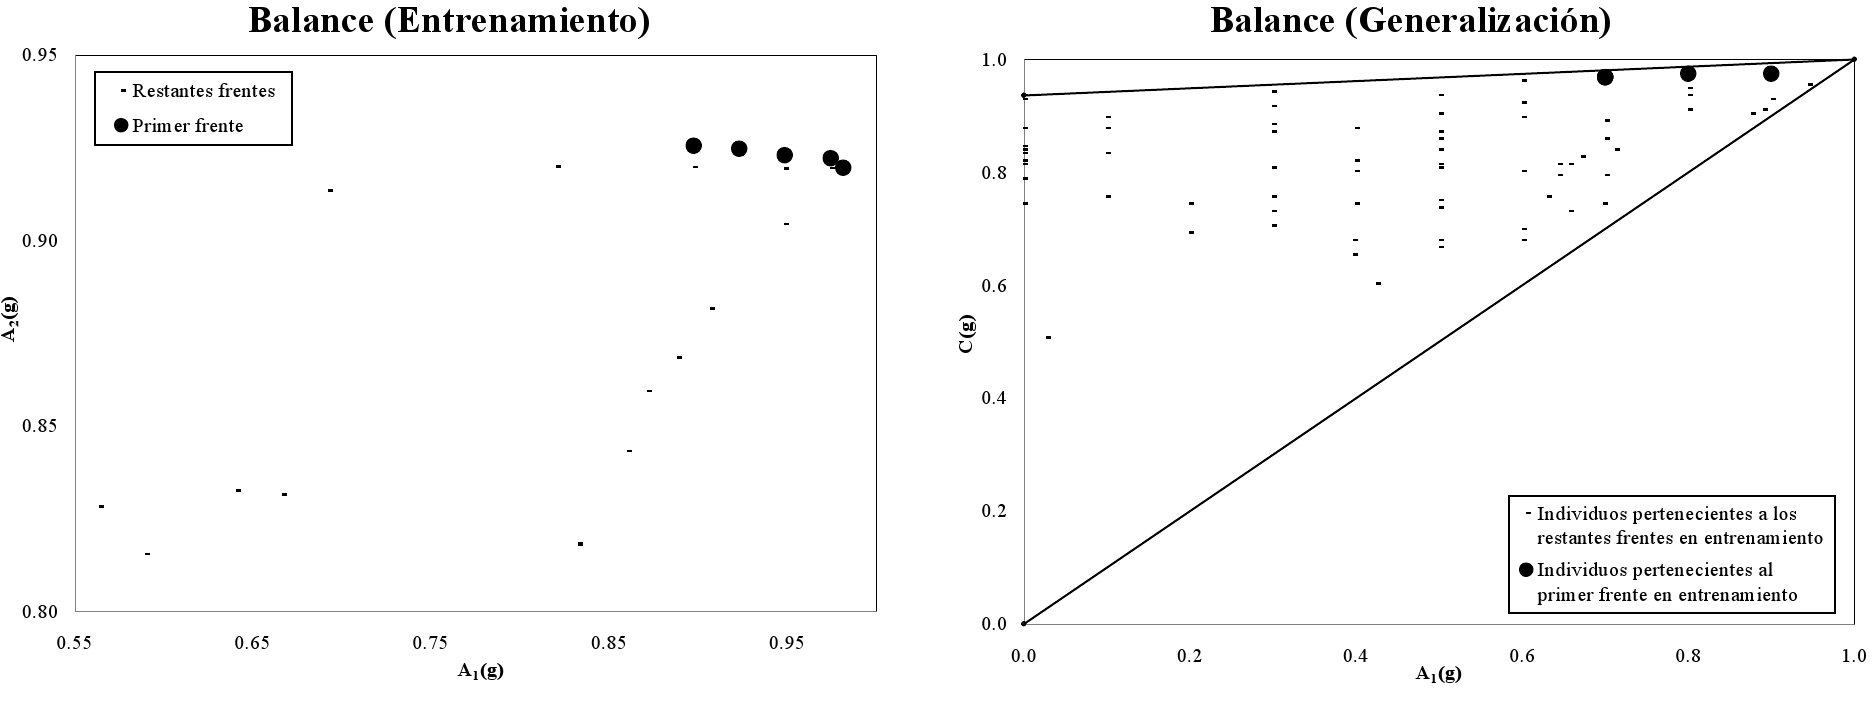
\includegraphics[keepaspectratio,width=18cm]{figuras/balanceEnsembles.jpg}
\caption{Frente de Pareto en entrenamiento $(A_{1},A_{2})$, y valores asociados a
$(A_{1},C)$ en generalización para el conjunto Balance.}
\label{figura1Ensembles}
\end{figure}
\end{landscape}

\begin{landscape}
\begin{table}[htb]
%\renewcommand{\arraystretch}{1.2}
\tabcolsep 2pt
\caption{Resumen de resultados en generalización comparando el rendimiento de las tres
metodologías de
\textit{ensemble}: \textit{Majority Voting} (MV), \textit{Simple Averaging} (SA), \textit{Winner
Takes All} (WT).}
\label{tabla2Ensembles}
\centering
\begin{tabular}{ccccccccccccc} \hline
\rowcolor[rgb]{0.70,0.85,1}\textbf{Método} &
\multicolumn{12}{>{\columncolor[rgb]{0.70,0.85,1}}c}{\textit{\textbf{Conjunto}}} \\
\cline{2-12}
\rowcolor[rgb]{0.70,0.85,1}&
\multicolumn{2}{>{\columncolor[rgb]{0.70,0.85,1}}c}{\textbf{Balance}} &
\multicolumn{2}{>{\columncolor[rgb]{0.70,0.85,1}}c}{\textbf{BreastC}} &
\multicolumn{2}{>{\columncolor[rgb]{0.70,0.85,1}}c}{\textbf{German}} &
\multicolumn{2}{>{\columncolor[rgb]{0.70,0.85,1}}c}{\textbf{Ionosphere}} &
\multicolumn{2}{>{\columncolor[rgb]{0.70,0.85,1}}c}{\textbf{AustralianC}} &
\multicolumn{2}{>{\columncolor[rgb]{0.70,0.85,1}}c}{\textbf{Pima}} \\ \cline{2-12}
\rowcolor[rgb]{0.70,0.85,1}& $\mathbf{C(\%)}$ & $\mathbf{MS(\%)}$ & $\mathbf{C(\%)}$ &
$\mathbf{MS(\%)}$ & $\mathbf{C(\%)}$ & $\mathbf{MS(\%)}$ & $\mathbf{C(\%)}$ &
$\mathbf{MS(\%)}$ & $\mathbf{C(\%)}$ & $\mathbf{MS(\%)}$ & $\mathbf{C(\%)}$ &
$\mathbf{MS(\%)}$ \\ \hline
\rowcolor[rgb]{0.86,0.94,1}MV & 51.64 & 12.68 & 66.47 & 40.15 & 71.41 & 60.35 & 91.51 &
80.72 & 87.66 & 86.29 & 77.04 & 65.77 \\
\rowcolor[rgb]{0.86,0.94,1}SA & \textbf{88.93} & 17.33 & 69.01 & \textbf{41.11} & 74.18 &
\textbf{61.28} & 92.57 & 82.70 & 87.86 & 86.73 & 78.05 &
\textbf{66.51} \\
\rowcolor[rgb]{0.86,0.94,1}WT & 84.50 & \textbf{64.44} & \textbf{69.90} & 26.19 &
\textbf{74.62} & 41.33 & \textbf{92.84} & \textbf{84.79} & \textbf{88.38} & \textbf{87.40}
& \textbf{78.29} & 55.92 \\ \hline
\multicolumn{13}{l}{Los mejores resultados se muestran en \textbf{negrita}.}\\
\end{tabular}
\end{table}
% \end{landscape}

% \begin{landscape}
\begin{table}[!htb]
%\renewcommand{\arraystretch}{1.2}
\scriptsize
\tabcolsep 2pt
\caption{Media de número de neuronas y número de enlaces para cada método y
conjunto de las tres metodologías de \textit{ensemble}: \textit{Majority Voting} (MV),
\textit{Simple Averaging} (SA), \textit{Winner Takes All} (WT).}
\label{tabla3Ensembles}
\centering
\begin{tabular}{ccccccccccccc} \hline
\rowcolor[rgb]{0.70,0.85,1}\textbf{Método} &
\multicolumn{12}{>{\columncolor[rgb]{0.70,0.85,1}}c}{\textit{\textbf{Conjunto}}} \\
\cline{2-12}
\rowcolor[rgb]{0.70,0.85,1}&
\multicolumn{2}{>{\columncolor[rgb]{0.70,0.85,1}}c}{\textbf{Balance}} &
\multicolumn{2}{>{\columncolor[rgb]{0.70,0.85,1}}c}{\textbf{BreastC}} &
\multicolumn{2}{>{\columncolor[rgb]{0.70,0.85,1}}c}{\textbf{German}} &
\multicolumn{2}{>{\columncolor[rgb]{0.70,0.85,1}}c}{\textbf{Ionosphere}} &
\multicolumn{2}{>{\columncolor[rgb]{0.70,0.85,1}}c}{\textbf{AustralianC}} &
\multicolumn{2}{>{\columncolor[rgb]{0.70,0.85,1}}c}{\textbf{Pima}} \\ \cline{2-12}
\rowcolor[rgb]{0.70,0.85,1}& \textbf{Neuronas} & \textbf{Enlaces} & \textbf{Neuronas} &
\textbf{Enlaces} & \textbf{Neuronas} & \textbf{Enlaces} & \textbf{Neuronas} &
\textbf{Enlaces} & \textbf{Neuronas} & \textbf{Enlaces} & \textbf{Neuronas} &
\textbf{Enlaces} \\ \hline
\rowcolor[rgb]{0.86,0.94,1}MV & 8 & 40.13 & 3.96 & 56.83 & 3.76 & 192.63 & 4.96 &
161.73 & 2.96 & 133.43 & 79.8 & 704.16 \\
\rowcolor[rgb]{0.86,0.94,1}SA & 8 & 40.13 & 3.96 & 56.83 & 3.76 &
192.63 & 4.96 & 161.73 & 2.96 & 133.43 & 79.8 &
704.16 \\
\rowcolor[rgb]{0.86,0.94,1}WT & 8 & 40.13 & 3.96 & 56.83 &
	3.76 & 192.63 & 4.96 & 161.73 & 2.96 & 133.43
		& 79.8 & 704.16 \\ \hline
% \multicolumn{13}{l}{Media de número de neuronas y número de enlaces para cada método y
% base de datos.}\\
\end{tabular}
\end{table}
\end{landscape}
% Existen multitud de técnicas para la generación de un conjunto de clasificadores. Según
% Dietterich \cite{Dietterich2000} se clasifican en:
% \begin{description}
% \item[Técnicas de voto bayesiano (\textit{Bayesian Voting}):] Se basan en el teorema de
% Bayes considerando todas las hipótesis del espacio como parte del conjunto de
% clasificadores que forman el \textit{ensemble}, asignándoles un peso equivalente a su
% probabilidad posterior.
% \item[Técnicas de manipulación de los ejemplos de entrenamiento:] Este tipo de técnicas
% manipulan el conjunto de entrenamiento para obtener diferentes clasificadores a partir
%de
% diferentes hipótesis, por ejemplo el método de \textit{Bagging} \cite{Breiman1996} que
%se
% basa en el submuestreo con reemplazo del conjunto de entrenamiento para generar un grupo
% diferente de hipótesis, utilizando cada muestra obtenida como un conjunto de
% entrenamiento, o el método de \textit{Boosting} \cite{Brazdil2009}, donde se van
%generando
% clasificadores de manera secuencial, dándole más importancia a los ejemplos que fueron
% clasificados de manera erronea por el clasificador anterior mediante la asignación de un
% peso a cada instancia o patrón del conjunto de entrenamiento.
% \item[Técnicas de manipulación de los atributos de entrada:] En estas técnicas se suele
% llevar a cabo diferentes agrupaciones de los atributos de entrada para generar los
% clasificadores que forma el conjunto, pero tiene el problema de que solo suelen
%funcionar
% bien cuando los atributos de entrada son redundantes.
% \item[Técnicas de manipulación de las salidas:] Estas técnicas manipulan la clase de la
% instancia a la que pertenece un determinado patrón, por ejemplo, si el número de clases
% es grande se dividen en dos conjuntos, de manera que los patrones de entrada se
% re-etiquetan y se utilizan para entrenar al algoritmo de aprendizaje generando un
% clasificador. Si este proceso se repite $l$ veces se obtendran $l$ clasificadores.
% \item[Ténicas de introducción de aletoriedad:] Este tipo de técnicas se basan en la
% introducción de aletoriedad a la hora de obtener un clasificador, por ejemplo, en el
%caso
% de ANNs se podría entrenar una determinada red utilizando diferentes pesos iniciales
% antes del proceso de aprendizaje.
% \end{description}
% La clasificación propuesta por Dietterich considera que los conjuntos de clasificadores
% se forman a partir de un único algoritmo de aprendizaje, es decir, que los
%clasificadores
% generados son homogéneos (será también nuestro caso). Existe otra manera de generar
% conjuntos de clasificadores mediante la aplicación de distintos tipos de algoritmos de
% aprendizaje a la hora de generar el conjunto de clasificadores, siendo estos
%heterogéneos,
% como por ejemplo, el método \textit{Stacking} \cite{Wolpert}, donde se utilizan
%diferentes
% modelos entrenados con un solo conjunto de entrenamiento y diferentes algoritmos para
% formar un meta-clasificador en varios niveles, donde cada nivel sirve para proporcionar
% meta-datos de entrenamiento para un clasificador final. Hay métodos que utilizan
% secuencias de clasificadores, por ejemplo, la generación en cascada
% (\textit{Cascade Generalization}) \cite{Brazdil2009} es se basa en la creación de una
% secuencia de clasificadores donde las probabilidades de salida se van transmitiendo de
% uno a otro hasta llegar al último clasificador de los que forman el \textit{ensemble} y
% que clasifica una determinada instancia. El método de delegación (\textit{Delegating})
% \cite{Brazdil2009} también asume una secuencia de clasificadores, de forma la salida de
% cada patrón debe alcanzar un determinado nivel o umbral para poder ser clasificado,
% pasándose éste al siguiente clasificador en caso de que no se cumpla esa condición y
% delegando la decisión final a otro clasificador. Similar al método de delegación o
% \textit{Delegating} está el método de arbitrariedad o \textit{Arbitrating}
% \cite{Brazdil2009}, donde los clasificadores que forman el \textit{ensemble} se entrenan
% previamente sin modificar el conjunto de entrenamiento y la decisión final se toma en
%base
% a un valor de esperanza o confianza matemática que presentan las salidas de cada uno de
% ellos.
%
% \section{El algoritmo MPENSGAIIES}
% \noindent
% \subsection{Resultados}
% \noindent
% \section{El algoritmo del ISDA09}
% \noindent
% \subsection{Resultados}
% \noindent
% \paginavaciasincuerp